\documentclass[12pt]{article}

\usepackage{apacite}
\usepackage[longnamesfirst]{natbib}
\usepackage{geometry} %for setting up margins
\usepackage{url} %this package lets a url appear in the bibliography
\usepackage[english]{babel}
\usepackage[autostyle, english = american]{csquotes}
\MakeOuterQuote{"}  % the previous lines make it so that the quotation marks all appear the right way around 

%\usepackage{listings} %for inserting R scripts
%\usepackage{verbatimbox}

\usepackage{fancyvrb} %centre verbatim box

%for the figure stuff
\usepackage{subfig}
\usepackage{wrapfig}
%\usepackage{subfigure}
%\usepackage{subcaption}
\usepackage[justification=centering]{caption}
\usepackage[bottom]{footmisc}
% to set up the figures to be apa
%\captionsetup[figure]{labelsep=period,labelfont=it,justification=justified,singlelinecheck=false,font=doublespacing}
% add in font=doublespacing

\usepackage{fancyhdr} %Just used to make nice headers and footers 


\pagestyle{fancy}
\fancyhf{}
\fancyhead[LE,RO]{9 Month Report}
\fancyfoot[LE,LO]{Page \thepage}

\renewcommand{\headrulewidth}{2pt}
\renewcommand{\footrulewidth}{1pt}

\usepackage{graphicx}


\usepackage[normalem]{ulem} %this adds the \uline{} function which stops underlined titles from running off the page 
\usepackage{hyperref} % This package makes it so that your citations become hyperlinks to the web url provided or to the reference section... That's really cool [colorlinks=true,linkcolor=blue,citecolor=blue]

\geometry{a4paper, total={170mm,257mm}, left=20mm, top=20mm}
\usepackage{setspace}
\linespread{1.5} %says there's a problem but it seems to work for line spacing



%\title{\textbf{\uline{Thesis draft}}}
%\author{Warren James}
%\date{}

%\setcounter{secnumdepth}{0}

\begin{document}

\begin{titlepage}
	\centering
	%\includegraphics[width = number\textwidth]{image title}\par\vspace{1cm}}
	%this could be used to add the Aberdeen logo?
	{\scshape\Large The University of Aberdeen \par}
	\vspace{1cm}
	{\huge\bfseries Assymetry and the Absence of Patterns Do Not Encourage Optimal Decisions.\par}
	\vspace{1cm}
	{\Large\itshape Warren James\par}
	\vfill
	Supervised by\par
	Dr.~Amelia \textsc{Hunt}\par
	and\par
	Prof.~Ben \textsc{Tatler}\par
	\textbf{Word Count:} 12755
	\vfill
\end{titlepage}	

%\tableofcontents

\newpage
%ABSTRACT
\begin{center}
\section*{Abstract}
\addcontentsline{toc}{section}{Abstract}
\paragraph{} Previous experiments that have tasked people with deciding how best to allocate resources have suggested that people are generally suboptimal. People appear to be unable to recognise that, for more difficult tasks, they should prioritise the completion of one or two tasks rather than attempting to complete all tasks. In the present study, we attempted to investigate why this might be the case by breaking the symmetry of previous tasks by making one option more likely (\textit{Experiment 1}), or easier (\textit{Experiment 2}), and by removing a potential distracting factor (\textit{Experiment 3}). Across each experiment, participants failed to perform the tasks using the optimal strategy. None of the participants switched from trying to achieve both goals to focussing on one at an appropriate point. The results of these experiments suggest that this failure to appropriately allocate resources may be due to a reluctance to accept a sure loss. 
\end{center}

%\paragraph{Keywords:} Decision Making, Probability Matching, Spatial Averaging

% table of contents
\begingroup\singlespacing
\newpage
\tableofcontents
\newpage
\endgroup

% Introduction
\section*{Introduction}
\addcontentsline{toc}{section}{Introduction}

\paragraph{} We may often find ourselves with multiple tasks to complete but limited resources with which to complete them. For example, with in upcoming exam, students will often have a large amount of material to cover but only a limited amount of time to spend revising the subjects. How a student should divide up their time depends on how well prepared they are. A well prepared student would probably benefit from covering each topic an equal amount as they are already likely to succeed. On the other hand, a poorly prepared student may benefit from spending all their time on a subset ot topics and hope that the topics they revised for come up. %Exams often require that the student has a reasonable level of knowledge about all possible topics that may appear. However, often there can be a wide range of topics that are not always so easy to link and thus appear entirely separate. Some students may struggle with the topics that are going to come up, whereas others might be very confident in their chances of succeeding regardless of what actually appears in the exam questions. For these two hypothetical students, it does not make sense for them to approach these situations with the same strategy. The student that is already fairly confident would benefit more from dividing their time relatively equally across the subjects that may come up because they are already fairly prepared. However, the student with little knowledge may not be able to reach a suitable level of preparedness for the exam if they were to split their time. Instead, for this student, it may be more beneficial to instead be more selective in what they study and primarily focus on one topic in the hope that topic will be in the exam. 

\paragraph{} Implementing this logic may seem fairly straightforward; if every task is difficult, it is a good idea to focus on only a subset, whereas when the tasks are straightforward, it makes sense to instead attempt a larger number. However, in tasks that present scenarios in which this logic should be applied,  people demonstrate an inability to switch from attempting both goals in an easy context, to focussing on one when they are both difficult \citep{clarke2015failure,morvan2012human}. By not following this relatively simple logic, the rate of success can fall far below what would be expected should the optimal strategy have been implemented. 

\paragraph{} It is assumed by the Expected Utility Theory (EUT) that people generally aim to maximise the utility of their actions; in other words, we tend to choose a course of action that would be most beneficial to us \citep{mongin1997expected}. When faced with uncertain, or risky, prospects, EUT suggests that we should pick the option that would be expected to give the decision maker the greatest rate of return. However, even before considering empirical evidence, it is possible to demonstrate that this theory can become incredibly hard to implement. \cite{BOSSAERTS2017917} discuss a thought experiment about shopping in which a person is expected to enter a shop and select the groceries that fulfil their criteria whilst also offering the maximum value. In their thought experiment, this shop only contains 100 items but this still offers a very large amount of comparisons to be made ($10^{30}$ comparisons). Considering this, it is possible to argue that the EUT is unlikely to explain behaviour very well when it comes to instances where there are a large number of options to choose from. 

\paragraph{} As mentioned above, using the EUT can entail some very computationally complex comparisons being required which would simply be beyond the scope of human beings \citep{BOSSAERTS2017917}. However, this does not mean that we can simply say human beings are irrational because we cannot implement this approach all the time. Instead, we must begin to consider that there are limitations to what human beings are able to do \citep{simon1990invariants}. This is the idea of \textit{Bounded Rationality} which posits that these limitations are important to consider when looking at human rationality. Instead of being "objectively optimal", perhaps we are behaving in such a way that accounts for our ability. Making $10^{30}$ comparisons might be simply too daunting and therefore we may instead opt for a much more simple approach. 

\paragraph{} When it comes to smaller problems, it is feasible to implement a strategy that compares the expected outcome across multiple choices. However, \cite{KahnemanProspect} present evidence that suggests that this is not the case either. In their work, they presented people with two choices; \textit{Option A} offered participants a $50\%$ chance to win \$1000 and a $50\%$ to win nothing, and \textit{Option B} would give them \$450 for certain. Using the EUT, Option A is the better option as this would on average reward the participant \$500. However, this was not the observed pattern of behaviour for most participants who instead would opt for \textit{Option B}. Perhaps more interestingly, they found that framing problems such as these would result in a shift from the sure option, to the more "risky" option. When framing this decision as being a loss rather than a gain, participants would instead opt for \textit{Option A} which in this context would be the worst option as is offers the greatest average loss. It can be argued that since the choices people make can be altered by simply changing the way a problem is framed, we are not simply comparing options and choosing the one that offers the best outcome \citep{KahnemanChoicesValuseFrames}.

\paragraph{} The issue with these sorts of tasks is that they are hypothetical \citep{KahnemanProspect}. Participants are supposed to imagine they are in a situation where choosing either option would result in one of the two stated outcomes. The question arises; what if people are put in a situation in which they are making decisions with actual outcomes? Until this point, the tasks considered have been hypothetical and are rarely (if ever) encountered in everyday life. As such, it would make more sense to look at decisions that people make many times a day. One task that fills this criteria is visual search. Whilst looking for something, we often aim to look in the places that are most likely to contain the item of interest. \cite{najemnik2005optimal} suggest that the way in which we scan a visual scene reflects that of an optimal strategy in that we choose to fixate the locations that are most likely to guide us towards the target or offer us the most information. By creating a model that accounted for the underlying statistics of a scene and the limitations of visual acuity, they argued they were able to predict eye movement patterns that closely resembled those of humans. Therefore, they argued that as performance of the ideal observer and human observe were very similar, we may be doing something close to optimal when directing our eye movements to locations within a scene.

\paragraph{} The model presented by \cite{najemnik2005optimal} suggests that humans are able to account for their own limitations and perform a complex task in an almost optimal manner. Should people be able to perform in the task of searching a visual scene optimally, then it should logically follow that doing this in a more simple scenario should also be possible. However, a study by \cite{morvan2012human} appears to demonstrate that this is not the case, and instead people struggle to account for their own visual acuity in order to make a decision that would reap the highest reward. 

\paragraph{} The task employed by \cite{morvan2012human} made use of a very simple display containing three boxes; one central with two on either side equidistant from the central box. This distance would change from being very close to being very far apart. Participants were tasked with detecting a target that would appear in either the left or right box (with equal likelihood) at the top or the bottom (again, with equal likelihood) and were tasked to state whether this target was at the top or bottom. Participants were told that they could fixate any of the three boxes displayed on screen but that the target would only ever appear in one of the two flanking boxes. The logic with regards to allocating resources can be applied here; when the boxes are close together (easy), then one should fixate the central box as it is possible to use peripheral vision to see both boxes, however, when they are far apart, one should instead fixate one of the side boxes as visual acuity will drop off in the periphery. Using the knowledge that each there is an equal chance of the target appearing in either box at the top or the bottom, we can see that switching to focussing on one of the side boxes means that accuracy should be $\approx75\%$. Participants should be $100\%$ accurate for their fixated box and, due to chance, be correct $50\%$ of the time for the non-fixated box resulting in an average accuracy of $75\%$. For each participant, visual acuity was tested in order to calculate at what point the participant should have switched from looking in the centre to looking at the side in order to achieve the greatest accuracy.

\paragraph{} The results from \cite{morvan2012human} and the replication by \cite{clarke2015failure} (hereafter referred to as the \textit{Detection Task}) suggested that people were unable to perform this task in such a way that would maximise their success. Participants did not appear to vary their fixation locations as a function of distance which would be expected should they have employed the optimal strategy. These results were also present in two other versions of this task that were carried out by \cite{clarke2015failure}. These other tasks made use of the same problem, but presented in several different ways. Their reason for doing this was to investigate whether this failure to "solve" this problem was specific to eye movements. The first of these three tasks involved participants trying to recall one of two strings of digits that could be short and therefore easy to remember, or long and more difficult to remember (the \textit{Memory Task}). For short sequences, it is easy to recall both and therefore time should be spent on each sequence, whereas when the sequences were long, the entire presentation time should be spent learning one of the sequences. The other involved participants selecting a standing position in order to throw a bean bag into one of two hoops (the \textit{Throwing Task}). Again, the same logic could be applied in that when the hoops were close, one should stand between and equidistant from each hoop, but for larger separations, standing next to one would increase chances of success. In both of these tasks, participants were unable to change their strategy as a function of difficulty thus further replicating these results. 

\paragraph{} However, in the last task they used, participants were uniformly able to complete the task using the optimal strategy. This final task (the \textit{Reaching Task}) required participants to select from one of three chairs in order to reach for one of two bean bags that were positioned on a table \citep{clarke2015failure}. The chairs were spaced so that one was in the centre with two at either end of the table. Again, the same strategy should be employed; sit in the centre when the bean bags were close together, but choose one of the side chairs when the distance was large. For the \textit{Reaching Task}, participants simply had to know how far they could reach which is something that would appear to be very easy to estimate due to its more tangible nature. However, the other tasks required an understanding of a more abstract ability.

\paragraph{} This possibility was investigated in \cite{James2017} using the \textit{Throwing Task} with the added measure of what participants understood their ability to be. As it was possible that participants were aware of their own ability but were not using this information, half of the participants were asked to state after having selected somewhere to stand. This was added as a potential prompt for participants to make use of this information which may have potentially improved performance \citep{chang2014self}. The results of this experiment suggested that all participants had a very clear understanding of their own ability. Prompting participants to think about their accuracy on each trial also did not appear to make participants better able to solve the problem presented to them. The results of \cite{James2017} appear to suggest either a failing of \textit{Bounded Rationality} in that participants were not considering/using their knowledge of their ability to accuractely throw bean bags appropriately, or that they were simply more focused on other aspects of the task that may have caused them to ignore this information. In the four studies presented here, the aim was to investigate what aspects of the task may have interfered with the participants' ability to figure out the optimal strategy. 

\subsection*{Probability Matching}
\addcontentsline{toc}{subsection}{Probability Matching}
%This is just a temporary intro to this section that can be edited at any point depening on where it is positioned in the final version
\paragraph{} The first of these factors to be investigated is that of \textit{Probability Matching}. \textit{Probability Matching} is when people select each item based on the probability that it will appear. This is often regarded as a suboptimal behaviour as it does not offer the greatest rate of success \citep{Koehler2010}. An eaxmple of this would be if one was tasked with selecting between two options several times in a row. If option A would reward you 80\% of the time, and option B only 20\% of the time, the best course of action is to pick option A all the time as this would result in an average success rate of 80\%. Whereas trying to match the probabilities by selecting each option in proportion to its likelihood of success would only yield an average success rate of 68\%.

\paragraph{} On face value, this appears to be a misunderstanding of probability. However, if one is able to detect the likelihood of each event occurring, this information can be useful in making decisions about where to direct our efforts. In the original paradigm \citep{clarke2015failure}, each potential target was equally likely to become the actual target. One may compare this to the "\textit{Buridan's Ass}" in which a donkey is equally hungry and thirsty whilst being equidistant from a source of food, and of water. With this in mind, there is no reason to opt for one target over the other as they are both equally attractive. Having two equally likely targets to aim for may have caused participants in \cite{clarke2015failure} to rely more heavily on a centre strategy than they should have given the optimal solution to the task. Committing to one side or the other may have been seen as "too risky" in such an uncertain context and so it may have appeared safer to opt for a more central location. 

\paragraph{} One way in which this can be investigated is by introducing a bias for one side to become the target more often than the other. Essentially, this would provide participants with a "pattern" that could be learnt and used to aid them in making a decision. As discussed before, people have a general drive to seek out patterns in order to inform their decisions \citep{yellott1969probability}. This tendency to seek out and exploit patterns can be seen in peoples' tendency to "\textit{Probability Match}" \citep{Koehler2010}. For example, \cite{Koehler2010} conducted a study in which participants had to guess whether a coin had been placed under a red or green cup. Participants were presented with 10 pairs of cups (one red and one green), and were told that for each pair a coin had been placed under either cup. The experimenter told them that they had decided under which cup to place the coin by rolling a 10-sided die with seven green faces and three red faces. The participants then had to produce a list of 10 guesses as to which cup they believed contained the coin. In this case, strictly matching would result in an accuracy of $58\%$, whereas always selecting the most likely option (\textit{maximising}) would result in an average accuracy of $70\%$.  

\paragraph{} Clearly maximising produces the more favourable outcome, however in their study \citep{Koehler2010} a minority of participants opted for this strategy (in total, $22\%$ of participants were strict maximisers). The question arises as to why people may be opting for a strategy that does not grant the best chance of success. \cite{Gao2015} argue that by \textit{maximising}, you are accepting that you will make a sure loss for a minority of trials. As such, the only way to negate this sure loss is to predict the sequence accurately. They argue that people instead choose to \textit{probability match} as this will allows for a very slim chance to earn 100\% of the reward \citep{Gao2015}. 

\paragraph{} To investigate the idea that matching is the result of attempting to be $100\%$ accurate, \cite{Gao2015} conducted a study in which participants predicted whether a red or green light would be displayed. One of the lights would appear $80\%$ of the time and the other only $20\%$ of the time. In the experiment, participants were given the chance to earn a bonus reward if they managed to get a certain accuracy level over 5 trials. They were either told the bonus would be earned if they were $100\%$, $80\%$, or $60\%$ accurate. The hypothesis was that when participants were told the bonus would be awarded for achieving $100\%$ accuracy, then they should observe a greater tendency to opt for a matching strategy. 

\paragraph{} This is what they observed; participants in the $100\%$ condition did have a higher rate of strictly matching. They suggested that by giving participants the goal of aiming to be $100\%$ accurate, participants began to focus on overall accuracy rather than treating each trial as independent of the others, something they argue is more likely to result in matching behaviour \citep{Gao2015}. Thus, they argue that the tendency to engage in matching behaviour is similar to the idea of avoiding loss \citep{KahnemanProspect}. By always choosing the more likely option, it is possible to view this as accepting some sure losses.

\paragraph{} This idea can be linked to the paper by \cite{clarke2015failure} in which the probability for each potential target was $50\%$. It is possible that participants would view choosing to focus their attention exclusively on a single option as being too risky due to the other option becoming a sure loss. By remaining somewhat central, there is still a small chance to succeed should either target be selected, albeit a very small chance. By introducing a bias to one side, this may push the more likely option to be a sufficiently attractive option so as to become a more viable option. Further, by adding in a bias for one option to be more likely, this may cater to a natural tendency to seek out and attempt to exploit patterns \citep{gaissmaier2008smart,yellott1969probability}.

\paragraph{} In some respects, one might suggest that searching for a pattern \citep{wolford2004searching} or even learning the underlying probabilities is quite demanding \citep{kahneman1982judgement}. For example, in order to learn a pattern, you have to keep in memory a large amount of information about what came before in order to learn the structure of the pattern. As such, \cite{wolford2004searching} suggested that presenting participants with a secondary distractor task that disrupts this search for patterns should result in less probability matching. %Using evidence from split-brain patients (patients that had undergone a commissurotomy due to epilepsy) and those with damage to the left frontal lobe \citep{wolford2000left}, they suggested that this search for patterns was mainly carried out in the left hemisphere. Therefore, by occupying this side of the brain with another task, they hypothesised that this would result in greater maximising behaviours. 

\paragraph{} \cite{wolford2004searching} presented participants with the task of guessing whether a target would appear in the upper or lower portion of a computer screen. One of these locations would be biased to contain the target $75\%$ of the time, and the other would only contain the target $25\%$ of the time. Some participants would simply carry out this task as a control group. Others would have to perform one of two distractor tasks. The task they opted for to occupy the left hemisphere involved remembering the last three digits they had seen. Before each trial, a digit would appear, and at random points during the block they would be asked to recall the most recent three digits that had been presented. Additionally, other participants were presented with a 6 sided polygon and were asked to recall whether this was the same or different to the one they had seen previously. Participants performing the distractor tasks were told that inaccuracies would result in a reduction of their reward. Their results suggested that by giving participants a task that occupied the left hemisphere, they began to approach a maximising strategy. The results of this study suggest that disrupting the search for patterns had pushed these participants to behave in a more "optimal" manner. 

\paragraph{} As \cite{wolford2004searching} suggest, this search for a pattern may hinder performance in tasks in which there is no true pattern to find. In the context of \cite{clarke2015failure}, this may have interfered with participants using information about their own ablity to make decisions. Instead, they may have been attempting to figure out any patterns that they believed may have been present. %In study 2 of this paper, a bias for one side was included to examine whether participants would begin to make use of this information. The hypothesis was that in a context where each option is equally likely, we should replicate the results of \cite{clarke2015failure}, however, once a bias is added, participants would be more likely to prioritise this target and begin to opt for choosing to attempt one task rather than try to achieve both. 


\subsection*{Spatial Averaging}
\addcontentsline{toc}{subsection}{Spatial Averaging}

\paragraph{} As discussed above, it's possible that probability matching as a strategy may emerge from an attempt to avoid being unsuccessful \citep{Gao2015}. This can be seen as related to the idea of \textit{loss aversion} as described by \cite{KahnemanProspect}. Loss aversion occurs when people opt for an option that does not entail a high chance of losing. This can be seen with the option A vs. option B tasks as mentioned previously. This is argued to be evidence that losses are weighted more heavily than their equivalent gains making a small chance of success seem preferable even when this option would most likely result in a larger loss. In the context of the tasks from \cite{clarke2015failure}, it may be that participants are reluctant to commit to one target as this would ensure that should the other potential be the target for that trial, they would incur a sure loss. If the idea of loss aversion was to explain the participants suboptimal behaviours in \cite{clarke2015failure}, then this would result in participants selecting the position that gave them a more equal chance of success should either side become the target. This idea of reducing the chance of failure on a trial can also be observed in the speeded reaching literature which may offer insight as to why participants were (in general) hesistant to fully commit to one option or the other in \cite{clarke2015failure}.

\paragraph{} In a paper by \cite{CHAPMAN2010168}, participants were presented with a very similar task. In their task, two circles were presented on a computer screen equidistant from a central point. Participants were told that one of these circles was the target for that trial and that they were to reach for this one. However, it would not be made clear which was the target until the participant had initiated a reaching movement and they had to reach the target within a time limit in order for the trial to count. In the first experiment, these circles were equidistant from the centre of the screen with each circle having an equal chance to become the target. In this setup, the participants generally tended to make a movement that remained equidistant from each potential target, and once the target was selected, they would alter their trajectory and move towards the target. In a second study, the distance from the centre of the screen was different for the two potential targets, and so one could be positioned further out than the other. As such, the "central" point that maintained an equal distance from each potential target was shifted slightly towards the further out circle. As there is still no certainty about which potential target would be the true taret for that trial, it still makes sense to reach towards the midpoint of these two targets as both were still relatively easy to reach for. This was reflected in the participants' reaching trajectories as they now initiated a reach that drifted slightly towards the further out target, thus maintaining an equal distance from each potential target. 

\paragraph{} In their third experiment \citep{CHAPMAN2010168}, the display would contain three potential targets; one on one side and two arranged one above the other on the other side. Each target was equally likely to contain the target. As such, this meant that the side with more potential targets would contain the target item more often as there was more chance overall. In this context, there is a little more certainty as to where the target will appear and so it now no longer makes sense to reach to the midpoint that maintains an equal distance to each target. Instead, a more optimal motion would take into consideration the higher likelihood that the side with more potential targets would contain the true target. This was reflected in participants behaviour as their motions initially appeared to have a bias towards the side that was more likely to contain the target. 

\paragraph{} The results from \cite{CHAPMAN2010168} suggest that under circumstances of high uncertainty (i.e. having no reason to choose one side over the other) that participants behave in such a way as to maintain an equal chance of success at both potential goals. When there was more certainty (albeit slight), participants were able to make use of this information when reaching towards the screen. This could be used to explain why participants in the study by \cite{clarke2015failure} were less likely to focus exclusively on one potential goal even when this was the best option as there was a large degree of uncertainty. Due to differences in aims and methods, irect comparisons between these studies are difficult. For example, in \cite{clarke2015failure} the difficulty of the task could change, and thus participants would sometimes have to stop trying to maintain an equal chance of success and instead focus on completing one task. However, in \cite{CHAPMAN2010168}, there was no point at which participants should have switched from maintaining an equal chance to focusing on reaching for one potential target. Therefore, the question stands as to whether the patterns of behaviour observed in the two experiments described above from \cite{CHAPMAN2010168} were the results of participants employing an optimal strategy or not. Further, the whole reaching process occurred in a continuous fashion. Unlike in \cite{clarke2015failure}, participants did not make a decision where to position themselves and then perform the task, instead this happened as one motion.% A paper by \cite{Hudson2007probmove} is more similar to the paradigm used by \cite{clarke2015failure} and also adds further support to the idea that participants may be trying to maintain an equal chance of success. 

\paragraph{} In \cite{CHAPMAN2010168}, the point at which the display changed to reveal one of the two potential target locations to be the target occurred as participants released a button they were told to hold down prior to each trial. This caused the decision process to be in one motion rather than separated stages. However, in \cite{Hudson2007probmove}, the participants' reach had to pass a certain threshold before the display in their experiment would change to reveal the true target for that trial. By including this as a constant, it becomes somewhat easier to directly compare the design to \cite{clarke2015failure} as there is an initial point at which the participant "positions" themselves prior to performing the task. 

\paragraph{} The task employed by \cite{Hudson2007probmove} was slightly more complicated than that of \cite{CHAPMAN2010168} as now there were several columns that could all potentially contain the target item. Each of these columns consisted of many grey squares arranged in a 4$\times$25 squares grid. On each trial, a certain portion of these squares would illuminate to indicate that for this trial any of these could be the true target of the participants reaching motion. The squares that illuminated could be distributed in different ways in order to make some columns more likely to contain the target than others. For example, the central column may contain the majority of potential targets with few appearing in the other columns. Additionally, this certainty could be reduced by increasing the number of columns that would contain a large proportion of the potential targets. This meant that certainty could be manipulated whilst keeping the same location as the point participants should aim for in order to have the greatest chance of success (i.e. the middle column would still be the centre of the distribution). 

\paragraph{} Much like in \cite{CHAPMAN2010168}, the results from \cite{Hudson2007probmove} are similar in that participants appeared to take into account where the target was most likely to appear. However, when the most likely column was more extreme (i.e. one of the side columns) participants did not commit to moving towards these columns. Instead, they appeared to overweight the chance that one of the columns containing very few potential targets would contain the actual target for that trial. This meant that the point at which participants crossed the threshold tended to be closer to the centre of space than would have been expected should participants have given appropriate weights to each column with respect to the number of targets they contained. This suggests that participants were reluctant to forgo the reward in the eventuality that the target appeared in one of the unlikely conditions. The instead opted for a strategy that would maintain some level of success at achieving this unlikely target at the cost of reducing the chance to succeed at the more likely columns. With less certainty, there were other ways in which participants altered their reaching behaviours. For trials with high certainty (majority of targets clearly in one column), participants crossed the threshold at a higher velocity than when there was a lower amount of certainty (targets more evenly distributed through the columns). This somewhat reflects a more optimal strategy as participants would be more able to correct mid-reach in the lower certainty conditions where there is a greater chance that this would be necessary. 
% Does this certainty need to be mentioned just yet, or save that for the discussion?


\paragraph{} The results of these studies seem to share a common theme that has been mentioned above. We seem to dislike decisive actions when they raise the certainty of which a loss may occur \citep{KahnemanProspect} and instead we tend to opt for an action that will mediate this risk and provide some chance of success even at the expense of success elsewhere \citep{Koehler2010,Hudson2007probmove}. This reluctance to, in essence, write off one potential goal as unachievable may help to explain the behaviour for most participants in \cite{clarke2015failure}. Participants may be reluctant to exclusively focus on one target over the other as this (for the most part) reduces the chance of achieving the non-focussed goal to $0\%$.

\paragraph{} The results of both \cite{CHAPMAN2010168} and \cite{Hudson2007probmove} suggest that people were trying to give themselves a more evenly distributed chance of success. In \cite{CHAPMAN2010168} this was evident in how participants would tend to move towards a point that would give a roughly equal chance of success when there was an equal chance of either location becoming the target. This suggests that participants preferred more equal odds of success to having a hight chance of success for some (if not 100\%) and the other having a much lower chance of success (if not $\approx$0\%). Also, in \cite{Hudson2007probmove}, we can see how participants demonstrated a reluctance to move entirely towards the most probable location and instead favoured points that allowed for a small chance of success should the unlikely happen.

%\paragraph{} For this part, we can say that instead of removing any sense of pattern, the change here was to introduce a reason to choose one over the other. So the choice still remains, but there is a reason to select one position over the other.

%\paragraph{} Pretty much the first thing to look at here is the \cite{CHAPMAN2010168} paper as that gives a very nice illustration of how people spatially average. Also, there is a paper by \cite{Hudson2007probmove} has a very nice experimental design that links this to the next section quite nicely.


\subsection*{Patterns}
\addcontentsline{toc}{subsection}{Patterns}

\paragraph{} The above sections have suggested ways in which the symmetry of the problem can be broken in order to cause one side to be more attractive than the other. However, one fundamental issue with this has already been mentioned; the pursuit of patterns \citep{wolford2004searching}. This predisposition to search for patterns is evident in the way in which it can interrupt the use of more sensible strategies \citep{wolford2004searching}, and also means we can "detect" patterns that simply do not exist \cite{yellott1969probability}. An experiment in the paper by \cite{yellott1969probability} asks people to make a simple guess as to whether one of two options will appear next. Unbeknownst to them, the option they pick will always be the correct answer. After having carried out this experiment, the participants were asked to explain how they made their choices and whether they had detected a pattern. Despite none existing, participants were able to produce some fairly elaborate patterns that also matched onto the choices they had made during the task. 

\paragraph{} With this comes the question, are participants trying to detect a pattern when completing the tasks of \cite{clarke2015failure}? Within a task such as this, it is often difficult to persuade participants that the sequence is entirely random as people generally have a misunderstanding of what \textit{randomness} is \citep{Ayton2004}. This can be seen in two biases that people tend to possess. The \textit{Gambler's Fallacy} is the often erroneous belief that the next event has a higher chance to not be the same as the previous. For example, seeing a coin flipped 5 times and seeing it land showing heads after every flip does not increase the chances that the next flip will result in a tails, however, falling for the \textit{Gambler's Fallacy} would mean that people are more likely to suggest that tails will come up on the next throw. The other is the \textit{Hot-Hand Illusion} which is essentially the opposite. Instead of thinking that things will change, this is the idea that things should remain stable and so a long sequence of heads would increase (again, erroneously) the odds that the next event will also be heads.  

\paragraph{} \cite{KAHNEMAN1972430} suggest that the \textit{Gambler's Fallacy} is a result of us expecting to see something that is representative of the underlying probability. In essence, we expect the short-term to behave in the same expected way to the long-term. With enough coin flips, we should begin to see proportions that reflect the random nature of a coin flip. This is not the same for much shorter sequences, and as such, this may be where the \textit{Gambler's Fallacy} comes from. We may tend to believe that a short sequence should also match the underlying probabilities in the same way a long sequence would. However, this argument does not explain how the \textit{Hot-Hand Illusion} can arise; if we believe that all sequences should closely resemble the expected probability of each event's success, why would we expect there to be long streaks? \cite{Ayton2004} suggest that these phenomena emerge from slightly different contexts.

\paragraph{} Sequences of events such as the outcome of a coin toss or the outcome of a football match differ with respects to how outcome comes about. The coin toss relies on pure chance, whereas the series of football matches relies on the players' performance. This is what \cite{Ayton2004} argues causes one phenomenon to occur as opposed to the other. They argue that the \textit{Gambler's Fallacy} is more likely to occur when applied to mechanical events, and the \textit{Hot-Hand Illusion} will occur when there is an element of human performance. They tested this by presenting people with several sequence of outcomes that had a high rate of chance to change (i.e. the current observation will be different to the previous observation), or a low rate of change (i.e. high chance of there being repetitions). Participants were then to judge whether the sequence had come from a coin being flipped, or football team's performance in a tournament. Consistent with their hypothesis, their results indicated that people were more likely to attribute a sequence with a high rate of change (reflective of the \textit{Gambler's Fallacy}) to a more mechanical/random source. 

\paragraph{} Interestingly, their results also appeared to show that when there was a $50\%$ chance of change (i.e. equal likelihood), participants were more likely to attribute this to human performance which suggests that no only are we prone to certain biases in certain contexts, but we also cannot recognise "true random" as being random \cite{Ayton2004}. This idea is not uncommon in Psychological literature and there are a wide range of studies that suggest humans struggle to produce random sequences \citep[see][for a review]{BARHILLEL1991428}. We also tend to believe that a random sequence should not contain long strings of repetitions and there should be a high rate of alternation between each potential event. 

\paragraph{} Some have argued that people often appear to define randomness as being an absence of any discernable pattern \citep{lopes1987distinguishing}. For example, even though it's equally likely that flipping a coin 8 times will produce a sequence of exclusively heads as a sequence that has a mix of heads and tails (e.g. "HTTHHTHH"), people will still tend to believe that the latter example is "more random" than the other \citep{KAHNEMAN1972430}. In both these examples, the sequence is equally likely to occur, however, people tend to not recognise that a truly random sequence of coin flips could result in heads for every flip. \cite{GRIFFITHS201885} argues that this tendency to seek out a pattern results in us underestimating how stable a random sequence can be. In their paper \citep{GRIFFITHS201885}, they present a model that was tasked with deciding whether a sequence was randomly generated or generated by some sort of rule. They were attempting to match human performance in this task in that we tend to look for a higher rate of change before stating something is randomly produced \citep{Ayton2004}. In their model, they included run length and symmetry as factors in order to decide whether a sequence had been produced by a something random (e.g. a coin toss), or by other means. By incorporating this sensitivity to run length and symmetry, they were able to closely reproduce the average response of participants performing a similar task. This suggests that we have a great deal sensitivity to any perceptible patterns which in turn biases us towards believing that there is a pattern present even when there is none. 

\paragraph{} In \cite{clarke2015failure}, each potential target had a $50\%$ chance of becoming the target on that trial. Each alternative having a 50\% chance to become the target is not always perceived as being the result of random processes due to biases that people possess \citep{Ayton2004}. As such, participants may not have believed the generated sequence to be random and thus engage in a search for patterns. As discussed before when considering probability matching, the search for patterns can be cognitively demanding and distract people from making decisions that maximise utility \citep{wolford2004searching}. Therefore, there is the potential that participants were instead focussing on detecting a pattern rather than making use of information that was present and would be useful in raising their rate of success. 

\subsection*{Financial Incentives}
\addcontentsline{toc}{subsection}{Financial Incentives}

\paragraph{} It is also possible that some participants lack the incentive to perform the task to the best of their ability. \cite{phillips1966conservatism} investigated this idea by tasking participants with estimating whether a bag they had been handed contained predominantly red or blue chips. They were told there were 10 bags in total with $X$ containing predominantly red chips and $10 - X$ containting predominantly blue chips. They were then told that the bags that contained mainly red chips either contained 70\% red chips and 30\% blue, or 60\% red and 40\% blue with the inverse of these being true for the predominantly blue bags. They were then presented with 20 chips from the selected bag and were asked to give an estimate of how likely the bag the chips were drawn from was a majority red or majority blue bag. What they found was that participants estimates were fairly conservative when compared to what would be expected via Bayesian inference. They questioned whether this could be due to a lack of incentive to perform this task more effortfully. 

\paragraph{} They then repeated this experiment but with a payoff schedule associated with their performance in the task. What they found was that the participants that were offered an incentive to be accurate demonstrated a higher amount of learning. This meant that later in the experiment, they would offer more accurate estimates than compared to the unpaid participants. However, they still remained somewhat conservative. 

\paragraph{} Another example of a payoff structure altering the behaviour of participants can be seen in \cite{Goodnow1955} in which participants that were rewarded for performance were more likely to employ a more optimal strategy. They tasked participants with making judgements of which event would occur on each trial. The likelihood of each event occuring was set in one of three ways; being equally likely, a 70\% bias in favour of one event, or a 90\% bias in favour of one event occurring. Half the participants were told that the task was one of learning and that they were to uncover some underlying principle, whereas the other half were told that the task was one of gambling in which they were to place a bet on which event was likely to occur on each trial. They found that participants in the gamble condition when there was a 70\% bias were more likely to opt for a \textit{maximising} strategy than those in the problem solving condition. This was also true for the 90\% bias condition, but the effect appeared less pronounced. 

\paragraph{} Although these studies do suggest that a financial incentive may have pushed some participants to perform the task in a more optimal way, it did not cause them to perform the tasks perfectly optimally. In a review by \cite{Camerer1999}, it is argued that a financial incentive is not entirely enough to remove all irrational behaviours. This can clearly be seen in \cite{morvan2012human} in which participants receieved a small sum of money for every successful trial. Despite this financial incentive, participants did not appear to behave any differently to those in \cite{clarke2015failure} who did not pay their participants any amount for successful trials. 

\paragraph{} However, it is possible that in the original setup employed by \cite{morvan2012human} that participants were still likely to seek out locations that provided them an equal chance of success, or they may have still seen the task as something of a problem to solve. As such, we feel there is still scope to introduce a financial incentive in such a way that would be able to investigate other ideas. 

\paragraph{} For example, as mentioned before, participants may simply be demonstrating a loss aversion habit in choosing to stand more central to stand rather than comitting to one or the other. Similar to as discussed above, both targets were initially of the same value either in their actual potential worth \citep{morvan2012human} or in their odds of containing the target \citep{clarke2015failure} and as such this may cause participants to follow a pattern of selecting a location to give a reasonably similar chance of success for both potential targets. 

\subsection*{Current Research}
\addcontentsline{toc}{subsection}{Current Research}

\paragraph{} The above sections all discussed potential influences on behaviour that may interfere with a participants ability to perform optimally in the tasks presented by \cite{clarke2015failure}. In the current paper, we intended to investigate the whether probability matching, sptial averageing, or a search for patterns may be able to explain the majority of participants' results. Each of the experiments in this paper aimed to investigate these different concepts' influence on how participants performed in the task. 

\paragraph{} In \textit{Experiment 1}, unequal probability was introduced into the design in order to investigate whether participants were in fact attempting to make use of this information. Additionally, this is also a somewhat abstract way to make one option more attractive than the other and thus remove the issue of not being able to decide which target to select. The aim of this study was to investigate whether participants would be able to incorporate this probability information into their decisions. As one option would now be more likely, the other could be ruled out even before considering the difficulty of the task at hand. The hypothesis was that in a context where each option is equally likely, we should replicate the results of \cite{clarke2015failure}, however, once a bias is added, participants would be more likely to prioritise this target and begin to opt for choosing to attempt one task rather than try to achieve both.  %Additionally, by making one option more attractive than the other, the problem size is somewhat reduced. One option would now be much more likely to result in favour than the other two and therefore could be ruled out even before seeing how difficult the task itself was. 


%\paragraph{} For \textit{Experiment 2}, the aim was to investigate whether participants were attempting to give themselves and equal chance at achieving each target regardless of which would become the target, much like in \cite{CHAPMAN2010168}. To do this, the relative difficulty of succeeding at each target was altered so that one side would be easier than the other should the participant position their self equidistant from both potential targets. However, if the participants were trying to give themselves and equal chance of success, they should have stood more closely to the more difficult target in order to equate their ability to succeed at both targets. 

%\paragraph{} Lastly, the two previous experiments still have the potential for participants to be distracted by the search for a pattern. \textit{Experiment 3} removed any potential for a pattern by offering participants the chance to attempt both goals regardless of what decision they made. The logic for performing optimally was still the same, as focussing exclusively on one potential target when the task was hard would still produce the greatest rate of success. The only difference here is that there is no potential for participants to be trying to figure out which target would be the actual target for that trial. 



%\paragraph{} There's surely something out there on pattern detection in sequences, as in how do people perceive randomness etc? There is a paper that talks about that but I can't remember the name. Also, it's probably good to mention the \cite{yellott1969probability} paper as well as that has the section on people seeing patterns despite there not being any present.

%\paragraph{} So we can mention that we removed the necessity to look for a pattern in the choices by giving them an attempt at both hoops each time.

%However, the pattern of maximising was unaffected by the accuracy level the participant was aiming for. 

% closing paragraph 
%\paragraph{} As such, this would appear to be another way in which people generally tend to opt for a sub-optimal strategy which does not maximise the utility of their decisions. 

% notes and potential sentences to use 
%\paragraph{} This idea of avoiding sure losses \citep{KahnemanProspect} could also be used to explain why participants were unlikely to opt for one side or the other in \cite{clarke2015failure}.

%\paragraph{} This is a more subtle version. It kind of combines making one the better choice whilst also introducing something pattern like. Although there is no pattern, there is an underlying reason to choose one side over the other.

%\paragraph{} So there are plenty of talking points in the lit review as well as in my 4th year thesis if you want to look there as well. 


% Should be split into several sections to talk about the different things we were looking at
% so in this case: Awareness of ability
%                  Spatial averaging (two ways)
%                  Probability matching


%\section*{Experiments preface}
%\addcontentsline{toc}{section}{Experiments preface}

% This can go at the end of the introduction or somewhere in there
%\paragraph{} The following procedures for each experiment are similar to those of the \textit{Throwing Task} (Experiments 1 and 2) and the \textit{Detection Task} (Experiment 3) from \cite{clarke2015failure}. All data analysis was performed in R \citep{R}. %For each task, the participants accuracy across different distances was modelled using the lmer function from the lme4 package \citep{bates2014fitting} in R \citep{R}.

% This might be useful to include at some point somewhere. Just a nice explanation of what the logic is behind the problem.
% Maybe change the example to be an economic one though?
% Or something that involves numbers to help prove the logic holds?



%\section*{Experiment 1: Awareness of ability \footnote{This experiment was actually conducted as my undergraduate thesis project. Due to the nature of the 9 month report being that this should be written to a standard acceptable for publishing and the intention of publishing these experiments together, this Experiment has also been included in this report.}}
%\addcontentsline{toc}{section}{Experiment 1: Awareness of ability}

%\subsection*{Methods}
%\addcontentsline{toc}{subsection}{Methods}
%\subsubsection*{Participants}
%\paragraph{} Twenty-four participants (17 female) took part in this experiment and were recruited via the SONA systems at the University of Aberdeen. All participants took part in return for course credit. The average age of participants was 19 (\textit{SD} = 1.5). The sample size allowed for 12 participants to participate in each condition which matches the previous experiment \citep{clarke2015failure}.

%\subsubsection*{Procedure} 
%\paragraph{} The protocol for this experiment was very similar to that of \cite{clarke2015failure}. The experiment took part over two sessions with a week between the first and second part. The experiment took place in a sheltered, paved area at the University of Aberdeen. The paving slabs measured 0.46m x 0.61m which allowed them to be used as a convenient metric by which to place the hoops as these fit neatly within these dimensions (the hoops had a diameter of 0.4m). 

%\paragraph{} In Session 1, participants threw 12 bean bags into a series of hoops placed at seven distances from a central location in two different directions. The hoops were evenly spaced from three (1.38m) to fifteen (6.9m) slabs away from the participant (see Figure \ref{fig:Session1-Throwing}). This was carried out in two different directions (hereby referred to as North and South) with the starting direction counterbalanced across participants. This meant that for each distance, the participant produced an accuracy score of \textit{x} out of 24 which was then used to model how the participant's accuracy decreased as a function of distance.

%NOTE 
% These figures have different x-axes... so you should update that as soon as

%\begin{figure}[ht!]
%	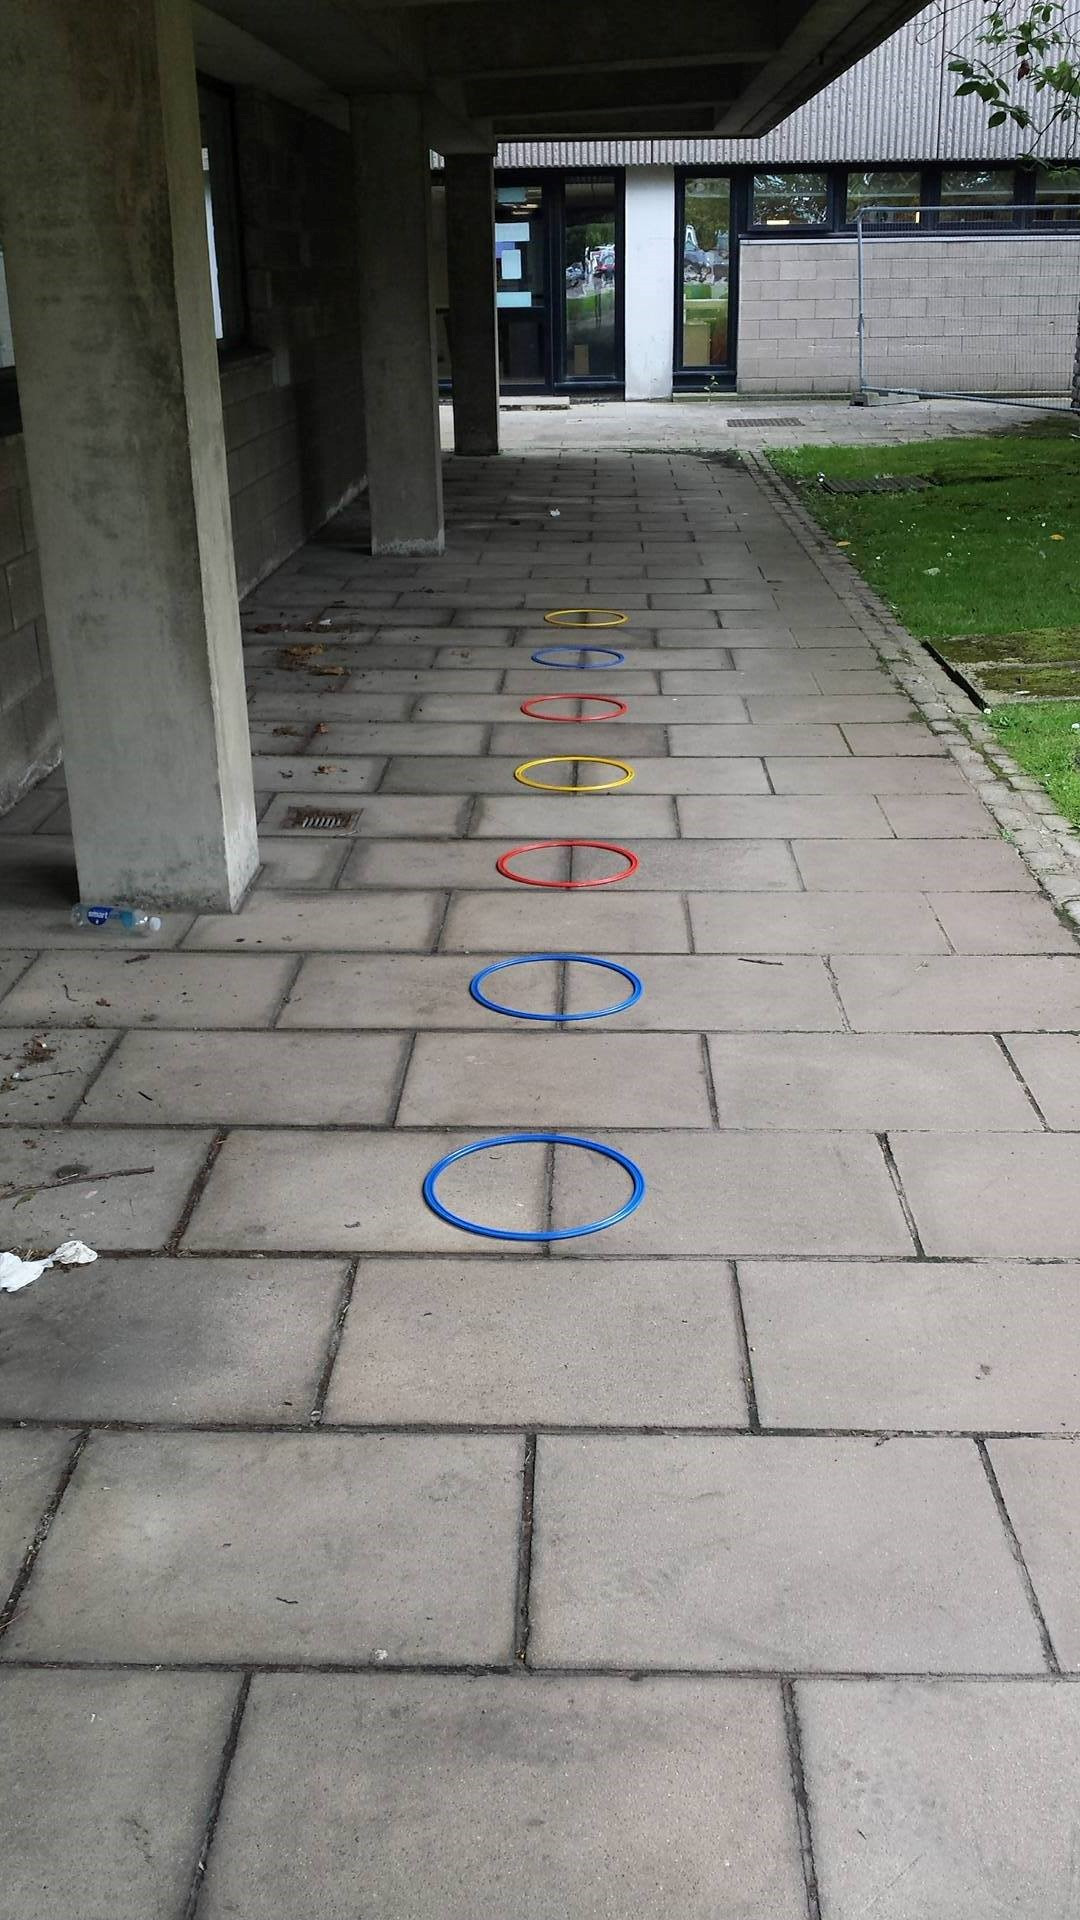
\includegraphics[scale=0.2]{Figures/Experiment_1_Awareness/Layout_part1}
%	\centering
%	\caption{This shows the set up for session 1 from the participant's point of view.}
%	\label{fig:Session1-Throwing}
%\end{figure}
%
%\paragraph{} Using the information collected in Session 1, we were able to calculate the distances at which participants were 10\%, 50\%, and 90\% accurate. This way the experiment was tailored to each individual's ability to accurately throw the bean bags into the hoops at different distances. These distances were then used to decide where the hoops were to be placed in Session 2. In this session, six hoops with 3 pairs defined by their colour were placed on the paved area (see Figure \ref{fig:Session2-Throwing} for the arrangement). Unbeknownst to the participant, each colour pair corresponded to one of the accuracy levels mentioned above (Red = 90\%, Yellow = 50\%, Blue = 10\%) as measured from an unmarked central position, equidistant from both hoops. 
%
%\begin{figure}[ht!]
%	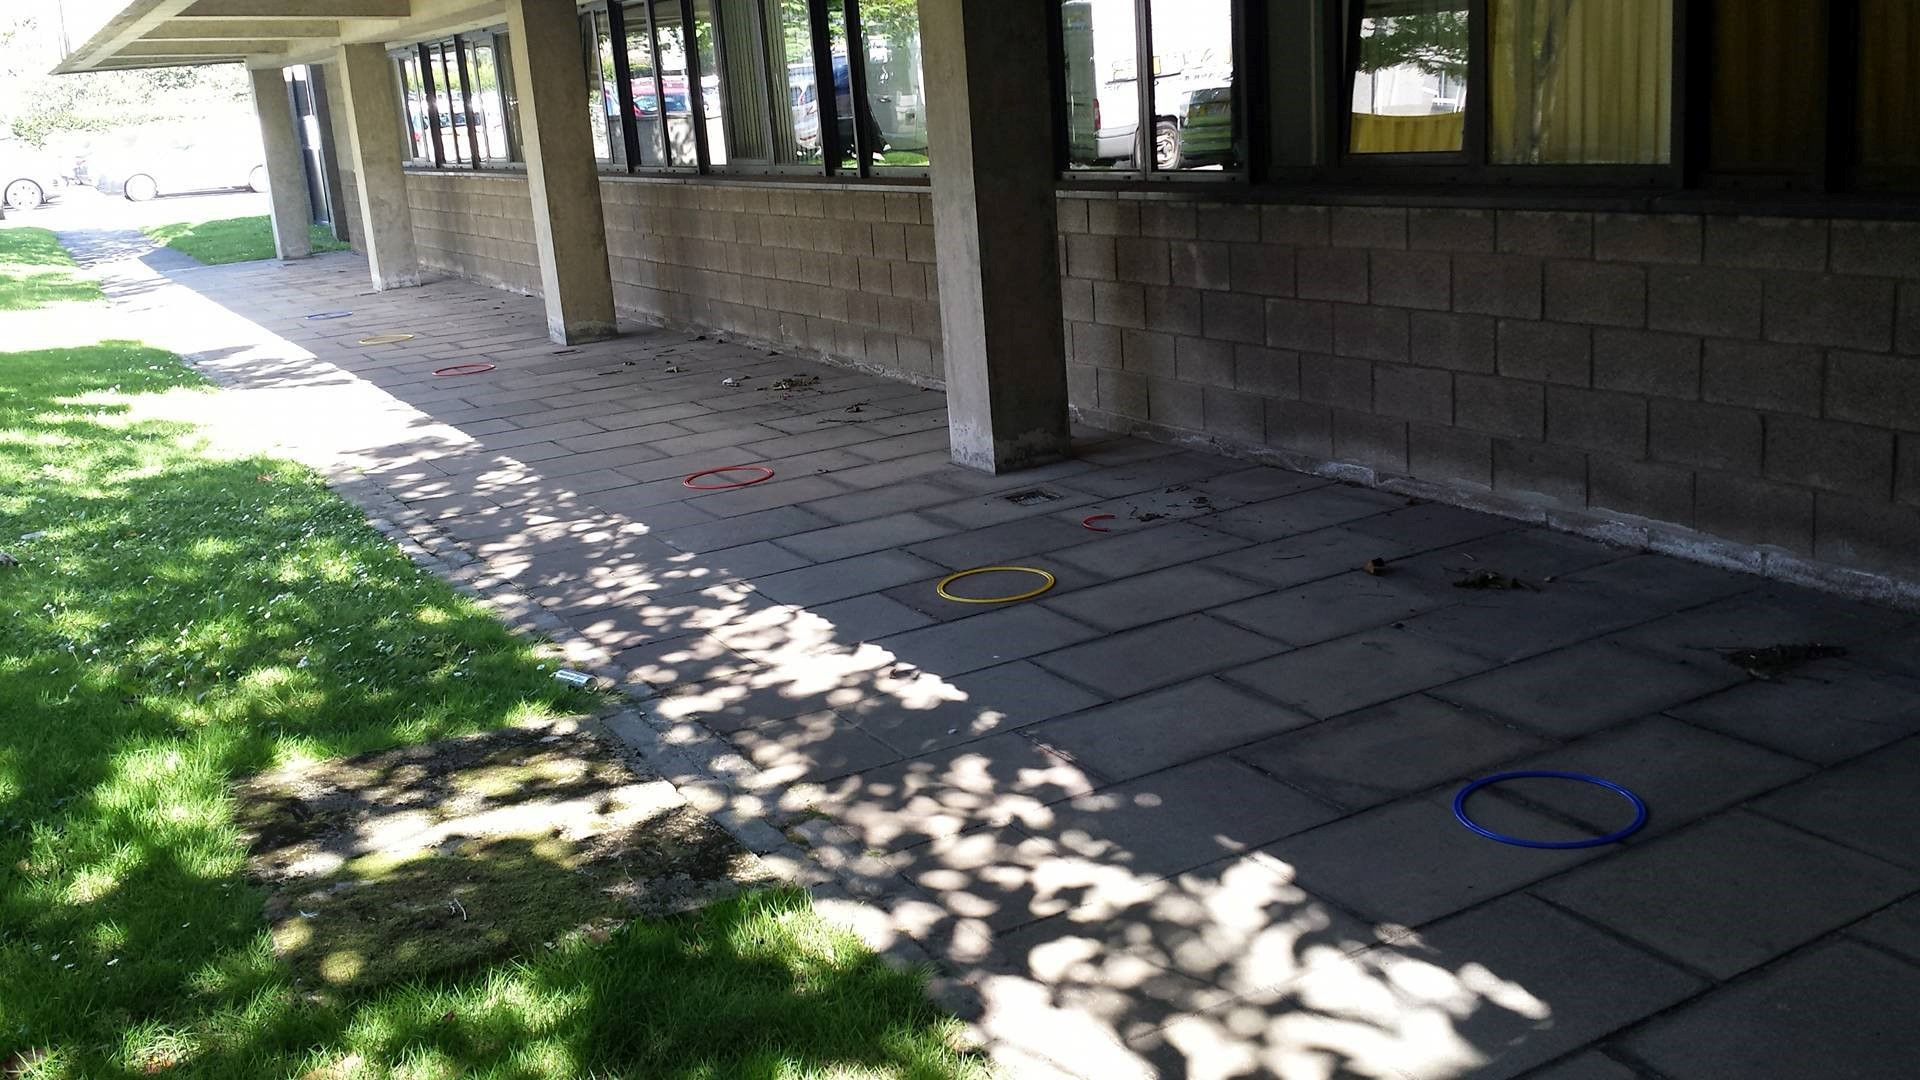
\includegraphics[scale=0.33]{Figures/Experiment_1_Awareness/Layout_part2}
%	\centering
%	\caption{The setup for session 2}
%	\label{fig:Session2-Throwing}
%\end{figure}
%
%\paragraph{} At the start of the experiment, the task was explained to participants. Their goal was to get as many of the bean bags into the stated target hoop (either north or south), but they would not be told which hoop was the target until they had selected where to stand. It was made clear to the participant that the direction of each throw had already been predetermined and was randomly generated. They were told they could stand anywhere on the paved area. Three bean bags of each colour were stored in a bag from which the participant would draw from before each trial. The colour of the bean bag would then indicate which pair of hoops the participants were to consider. The removed bean bag was not replaced until all nine had been thrown which ensured that there were an equal number of trials for each hoop separation. After drawing the bean bag, the participant would select a position to stand. This was then recorded in a covert manner before the experimenter stated whether they were to throw to the North or South on that trial.

%\paragraph{} This protocol was the same for every participant, however, half of the participants were asked on every trial to state what they expected their accuracy to be for each hoop from the position they had selected to stand. Participants were asked to give this as a percentage chance of success should each hoop be the target. This group will be referred to as the \textit{Online Estimation Group}. 

%\paragraph{} At the end of Session 2, all participants were then given one final task which was similar to Session 1 but did not require the participants to throw any bean bags. Participants stood at one spot and a single hoop was moved through several positions, at which point the participant was to give an estimate of their accuracy at that distance. The distances were split into two set: 3, 7, 11, 15, and 5, 9, 13. One of these sets was presented in an ascending order, and the other in a descending order with this counterbalanced across participants. 

%\paragraph{} After this, the participants were debriefed and had the solution to the problem explained to them. Participants were also encouraged to ask any questions they may have had about the experiment. 

%\subsection*{Results}
%\addcontentsline{toc}{subsection}{Results}

%\subsubsection*{Actual accuracy vs. Estimated accuracy}
%\paragraph{} 

%THIS plot needs to be made again but larger. At the moment it gets scaled up and doesn't look very nice... Should be easy enough to remake these plots.
%\begin{figure}[ht!]
%	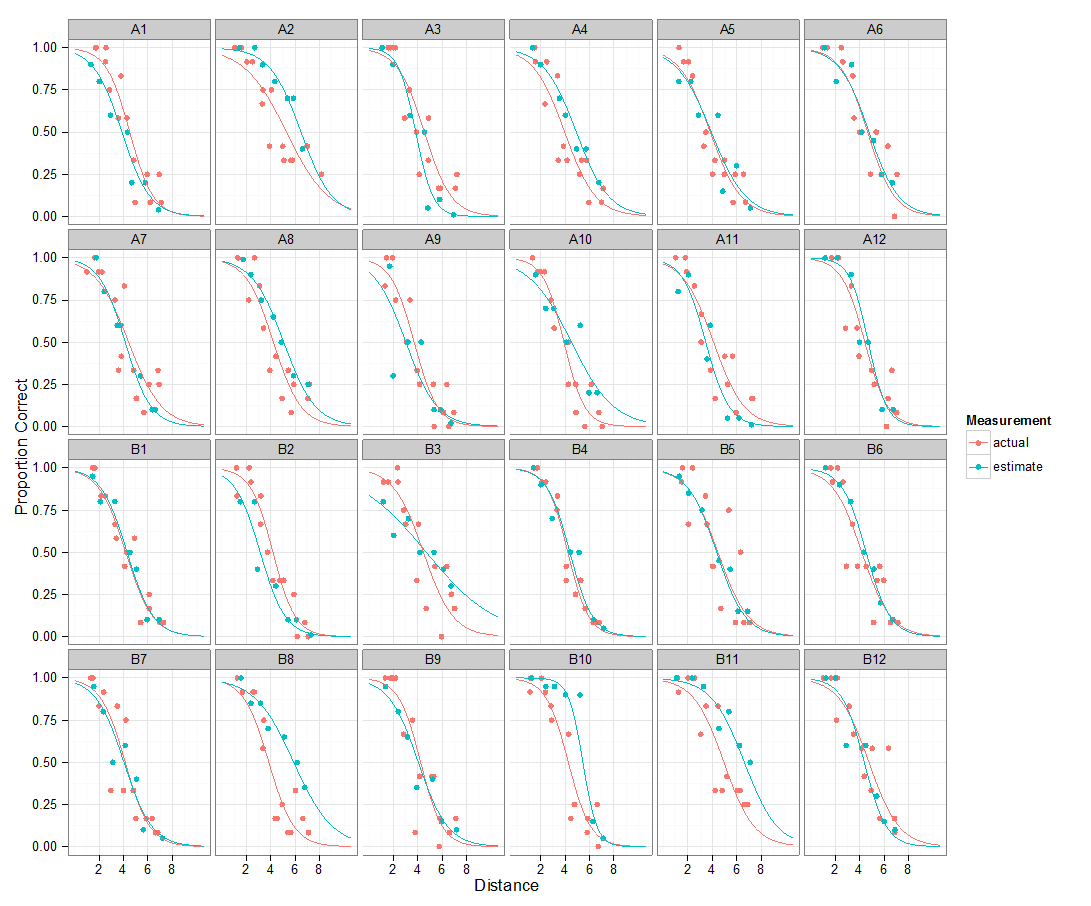
\includegraphics[width=\linewidth, height=8.5cm]{Figures/Experiment_1_Awareness/Compare_act_est}
%	\centering
%	\caption{These graphs illustrate the accuracy (proportion correct) over the various distances for each participant (actual accuracy, in red), and their estimates of their own accuracy over the same distances (in blue). }
%	\label{fig:Compare_act_est}
%\end{figure}

%\subsection*{Discussion}
%\addcontentsline{toc}{subsection}{Discussion}

%\section*{Notes}
%\addcontentsline{toc}{section}{Notes}
%\paragraph{} Remember to re-write the methods for Experiments 2 \& 3 as at the moment, the more in depth explanation of the paradigm falls in Experiment 3...

\section*{Experiment 1: Probability Matching}
\addcontentsline{toc}{section}{Experiment 1: Probability Matching}

\subsection*{Methods}
\addcontentsline{toc}{subsection}{Methods}
\subsubsection*{Participants}
\paragraph{} $10$\footnote{The aim was to have 18, but due to technical issues and an unusually high drop-out rate this was not reached. As such, any discussion of the results is preliminary at this time.} Participants (9 female) took part in this experiment, with an average age of 23 (SD = 3.2). Participants were recruited via word of mouth and posters. For participating in the experiment, participants were reimbursed \pounds10 for their time. 

\subsubsection*{Procedure}
\paragraph{} This experiment followed a similar structure to the \textit{Detection Task} from \cite{clarke2015failure}. The experiment took part over two sessions involving one to measure visual acuity, and the other for the participants to perform the decision task. The first session lasted approximately 30 minutes, and the second session lasted between 40-50 minutes.

\paragraph{} The experiment took place in a darkened room on a desktop computer. An Eyelink 1000 (version 4.594) (SR Research ltd, Mississauga, Ontario, Canada) was used to record eye position at 1000 Hz. In each session, a 5 point calibration was carried out with additional calibration and validation sequences prior to every block, and if the participant had broken fixation ten times cumulatively or for five trials in a row. The task was displayed on a CRT monitor with a resolution of 1920$\times$1080 using Matlab 7.9.0 (R2009b) with psychtoolbox \citep{brainard1997psychophysics,pelli1997videotoolbox} and EyelinkToolbox functions \cite{cornelissen2002eyelink}. A chin rest with forehead bar was used to ensure participants maintained a viewing distance of 47cm. 

\paragraph{} In the first session, participants were told that their task was to identify a letter that would appear in one of two boxes. All participants had to do was fixate a cross presented at the centre of the screen against a greyscale background and press the space bar. After a stable fixation of $700ms$, a target letter would appear in one of the two boxes for $500ms$. The Boxes were lighter shades of grey and occupied $1^{\circ}$ of visual angle. The letter would appear in the centre of one of these boxes and occupied $0.4^{\circ}$ of visual angle and was white. Two boxes were presented on either side of the fixation cross at several eccentricities ($3^{\circ}$, $4.3^{\circ}$, $5.8^{\circ}$, $7.5^{\circ}$, $9.3^{\circ}$, $11.1^{\circ}$, $12.5^{\circ}$, \& $13.7^{\circ}$; degrees of Visual Angle). Each separation was repeated $12$ times before moving onto another separation at random. After each separation had been cycled through, the participants were then offered a break before recalibrating and moving onto the next block. In total, participants completed 4 blocks of this. After the target had been presented, a screen would appear prompting the participants to identify which letter they thought they had seen. In this experiment, 10 letters were used all of which were drawn in the Sloan font as these letters are generally of equal recognisability at different viewing angles \citep{sloan1952comparison}. An illustration of each trial in Session 1 can be seen in Figure \ref{fig:Session1-Prob}.

\begin{figure}[ht!]
	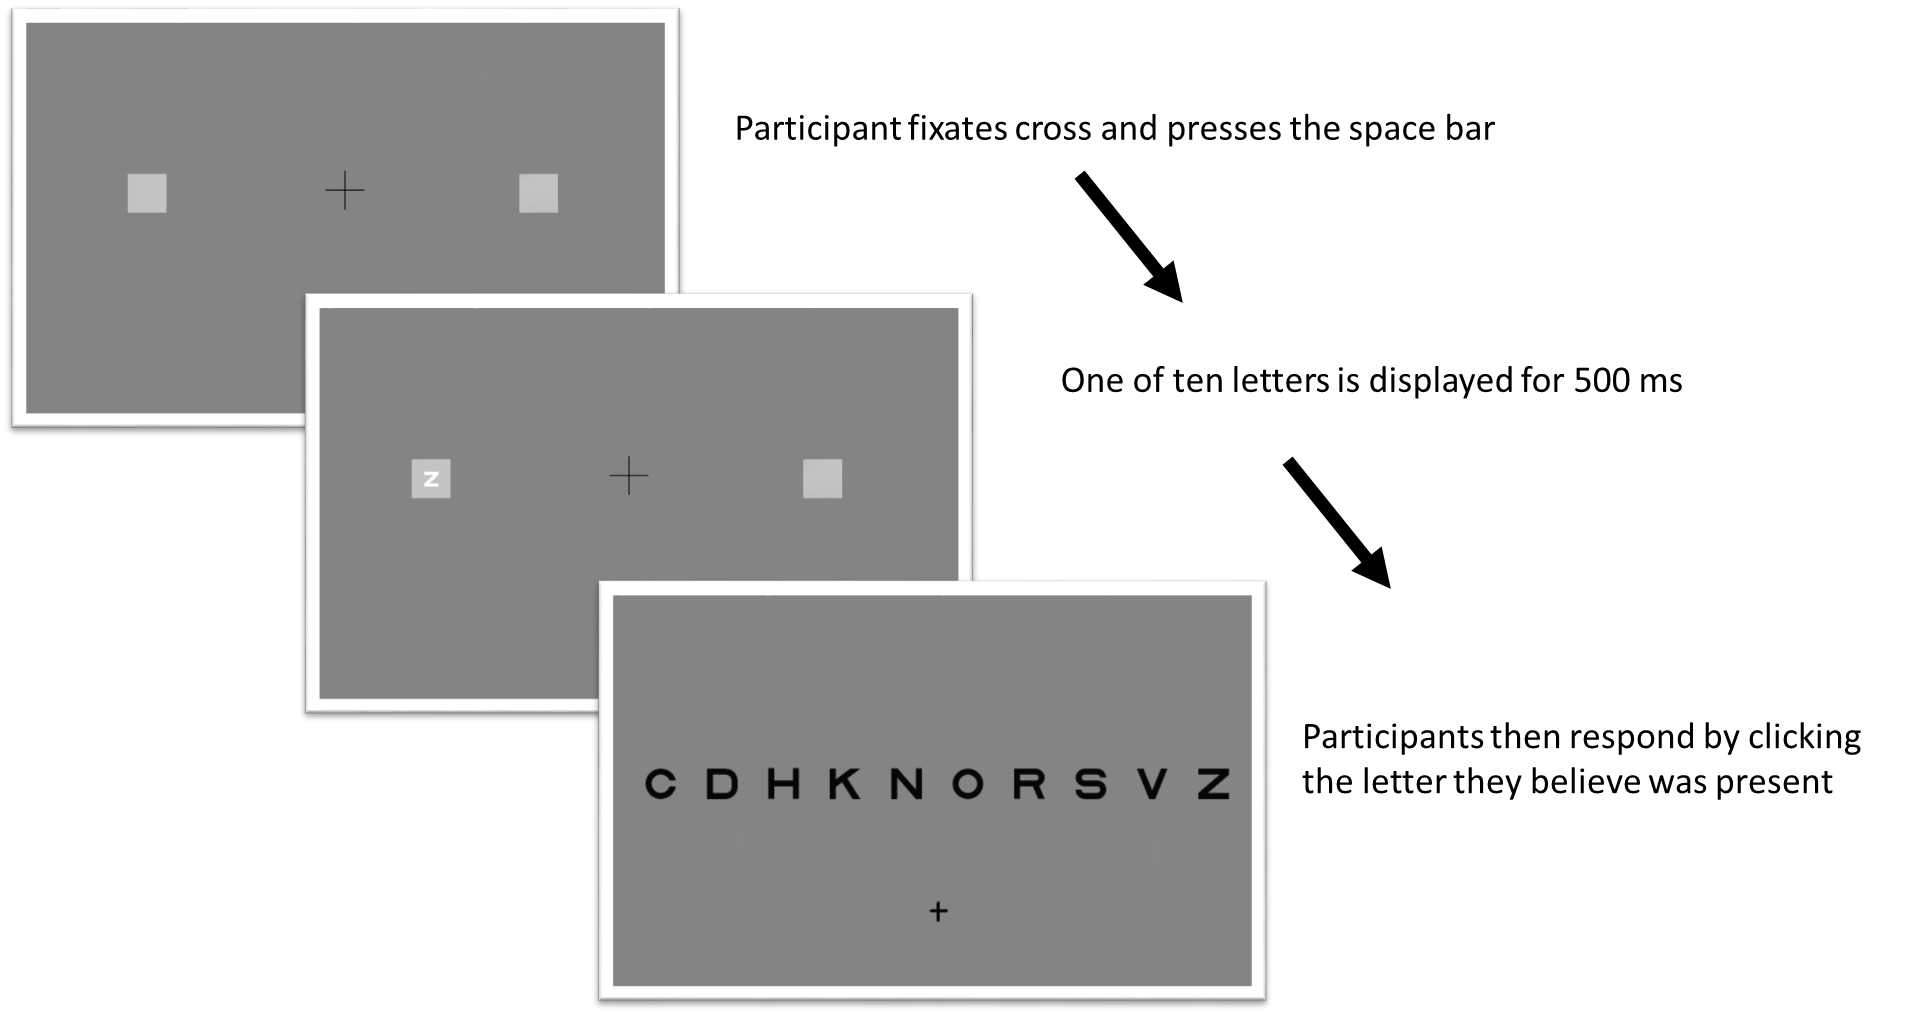
\includegraphics[scale=0.35]{Figures/Experiment_4_prob/Part1_Trial}
	\centering
	\captionsetup{justification=centering}
	\caption{The sequence for every trial in Session 1}
	\label{fig:Session1-Prob}
\end{figure}

\paragraph{} The results of this session were then used to tailor the separations that would be used in the participants second session. A \textit{"switch-point"} was calculated based on their performance and was used as centre point to then calculate the positions for several other separations. This switch-point was to ensure that every participant would have trials in which they should fixate in the centre and others in which they should switch to instead fixate one of the side boxes.

\paragraph{} The switch-point for each participant was calculated to be the separation at which the participant was $68.5\%$ accurate. From this point, 6 other separations were calculated by subtracting and adding 1, 2, and 3 degrees of Visual angle. There were two other points included which acted as anchors, one being a very large distance ($19.4^{\circ}$) and one being very small ($1.9^{\circ}$). The accuracy level of $68.5\%$ was decided upon as this is the mid-point between $55\%$ and $82\%$. These corresponds to the point at which participants should switch depending on whether the target was equally likely to appear on each side (\textit{Random}), or would appear on one side $80\%$ of the time (\textit{Bias}).

\paragraph{} Employing the optimal strategy would have allowed participants to achieve a certain level of accuracy. In the random condition, the target is equally likely to appear on either side, as such this means that should the fixate one of the side boxes, they have a $55\%$ chance of being correct. For example, the participant would achieve $100\%$ for the fixated box and $10\%$ chance for the other. If both boxes were equally likely to contain the target, we can calculate their expected accuracy by doing $(1 \times 0.5) + (0.1 \times 0.5)$ resulting in an average accuracy of $55\%$. This changes when there is a bias for one side to appear more often, though the logic still holds. The only difference is that now the probabilities change to reflect the bias. This is calculated by $(1 \times 0.8) + (0.1 \times 0.2)$ which results in $82\%$ accuracy.

\paragraph{} In Session 2, participants would fixate a cross that appeared above where the boxes would appear. The cross would appear at the midpoint between the centre box and either the left or right box with an equal chance. Once they had fixated the cross, they were instructed to press the space bar. After a stable fixation was detected for $700ms$, three boxes would be presented (Figure \ref{fig:Session2-Prob}). One box would appear in the centre with the other two spread equally on either side with a separation as calculated for that particular participant. Once these boxes had appeared, participants were instructed to fixate one of the three boxes. Participants were told that the target would never appear in the central box however they were free to fixate this location. After they had fixated one of the boxes, the letter appeared in one of the side boxes for $500ms$, after which the 10 letter stimuli were presented on screen for them to select which letter they had seen. Each separation appeared 10 times within a block meaning each block consisted of 90 trials. To ensure that each separation appeared equally, a list was produced containing 10 of each separation. This list was then shuffled so as to be in a "random" order.

\begin{figure}[ht!]
	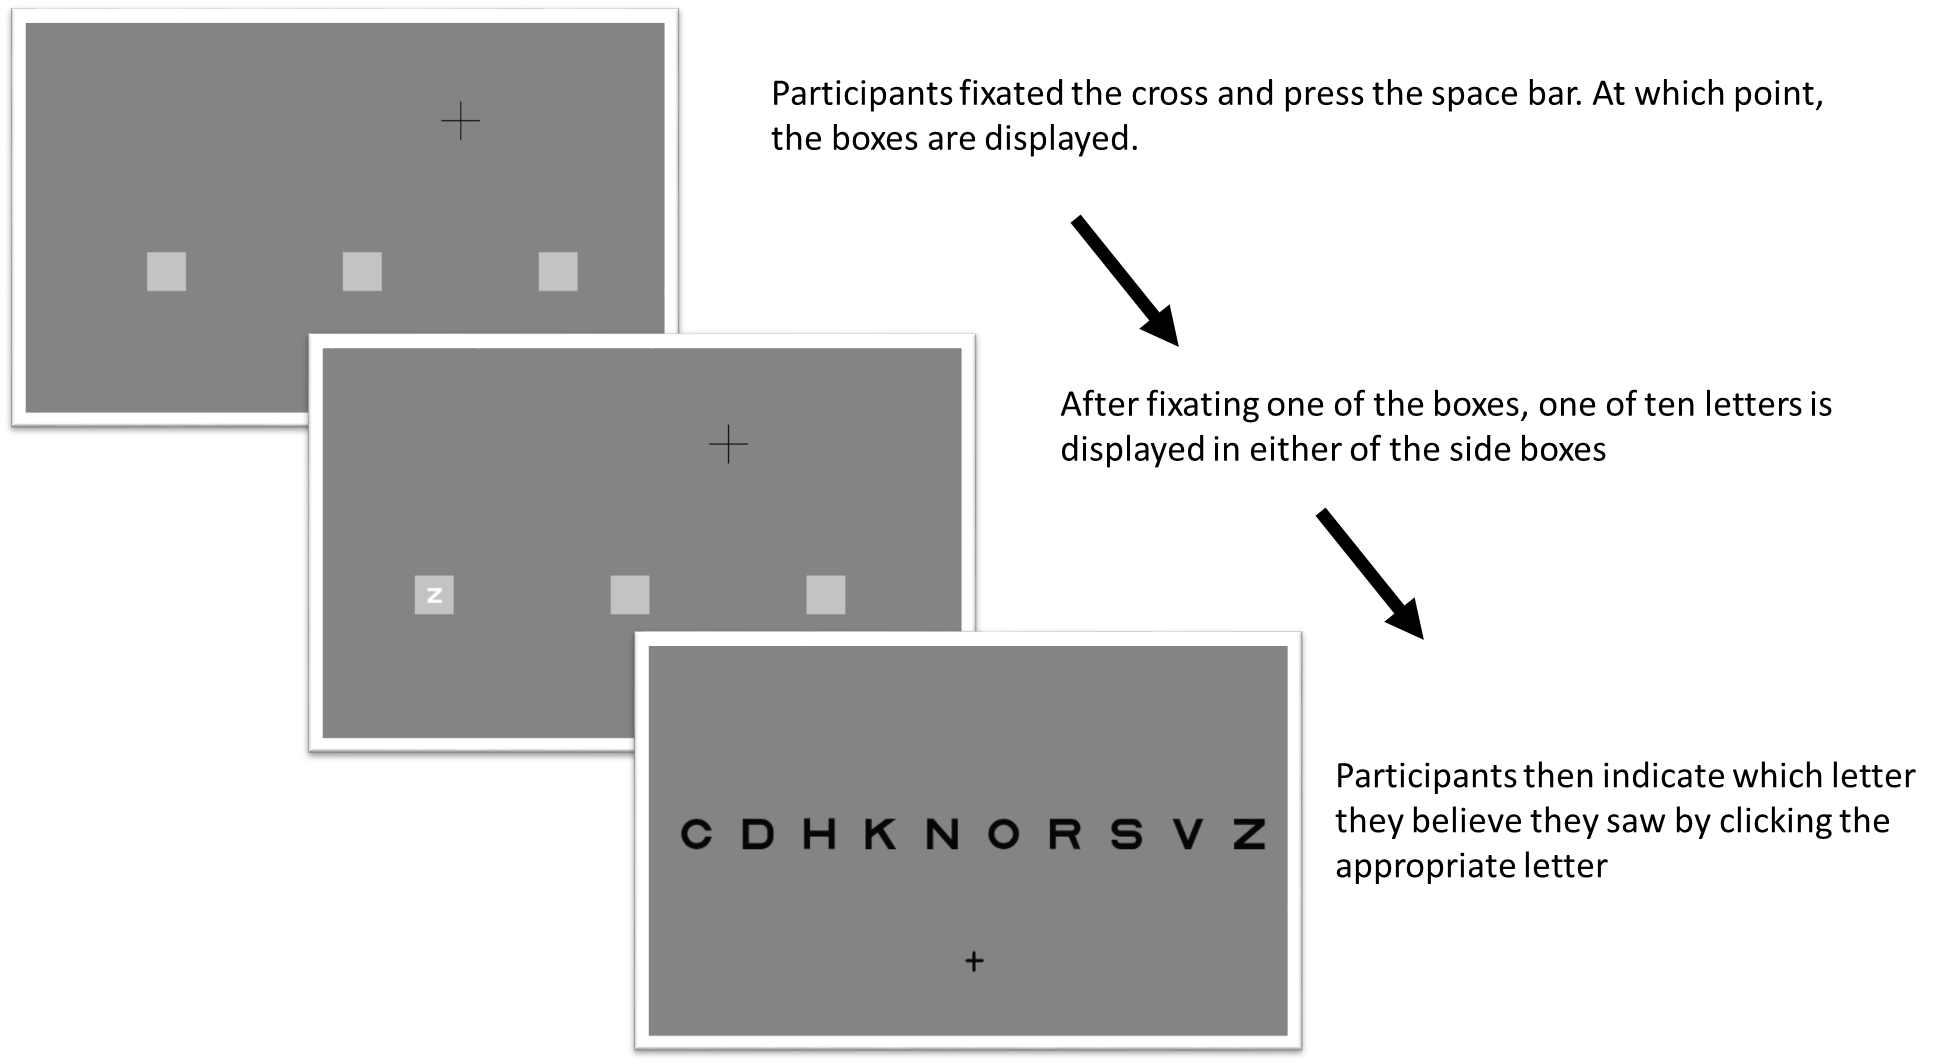
\includegraphics[scale=0.35]{Figures/Experiment_4_prob/Part2_Trial}
	\centering
	\captionsetup{justification=centering}
	\caption{The sequence for every trial in Session 2}
	\label{fig:Session2-Prob}
\end{figure}

\paragraph{} Prior to each block, participants were told how likely each box was to contain the target. There were two levels of probability; one in which each box was equally likely to contain the target on each trial (\textit{Random}), and one in which one side would contain the target $80\%$ of the time (\textit{Biased}). Each participant took part in both the \textit{Random} and \textit{Biased}. Participants completed one condition for 4 blocks in sequence before moving onto the next condition. This order was counterbalanced across participants. Additionally, the side that was more likely to contain the target was also counterbalanced so as to account for any possibility that participants may have a bias to look to one side over the other. 

\subsection*{Results}
\addcontentsline{toc}{subsection}{Results}
\subsubsection*{Fixation proportions}
\paragraph{} All analyses for this and subsequent experiments were carried out using R \cite{R}. A General Linear Model with a binomial link was carried out in order to assess whether fixations towards the side boxes increased with a larger \textit{Delta}. As can be expected after looking at Figure \ref{fig:Session2-prob-props}, there was no significant effect of \textit{Delta} on fixation proportion. Additionally, including condition (i.e. \textit{Biased} or \textit{Random}) did not improve the fit. This may be expected given there is such a large variety of performance across the participants. It would appear from inspecting the plots that participants tended to follow a similar strategy regardless of context when deciding whether to fixate on the central box or one of the side boxes in both conditions. For example, participant 15  fixated exclusively on the side boxes, whereas participant 7 almost exclusively chose to fixate the central boxes (Figure \ref{fig:Session2-prob-props}). As participants appeared to follow a similar strategy regardless of condition, it does not appear that participants are more likely to fixate the side boxes when there is a greater reason to do so. Instead, they appear to be quite idiosyncratic in their behaviours. 

\paragraph{} Although participants did not appear to fixate the side boxes more when in the biased condition, there did appear to be a difference in which box was fixated. This was investigated by using a General Linear Mixed Effects Model with a binomial link. For this analysis, only fixations to the side boxes were included so as to compare the relative amount of fixations towards each side. The value being predicted was whether the participant chose to fixate the box that was more likely in the bias condition and that same box in the random condition (e.g. if the more likely box was on the left, the number of fixations to the left box was compared). The results of this model (seen below) indicated that condition had an effect on how often participants directed their attention to the more common box. In the \textit{Biased} conditions, participants were more likely to choose to fixate the common side than when they were participating in the \textit{Random} condition.

\begin{figure}[!ht]
	\centering
	\begin{BVerbatim}
	FixationsToCommonSide ~ Condition + (1|participant), family = binomial
	\end{BVerbatim}
\end{figure}

%This was tested using a McNemar's test to see if the proportion of saccades towards one side (i.e. the biased side) was greater in the \textit{Biased} condition than in the \textit{Random} condition. On average, participants did appear to direct their fixations to one side more often in the \textit{Biased} condition (M = 0.86) than in the \textit{Random} condition (M = 0.68); $\chi^2$(1, N = 10) = 60.785, p $<$ 0.001. %This was tested by using a paired-samples t-test, the participants' proportions of fixations to the side most attended were compared to see if being in the \textit{Biased} condition lead to a greater proportion of fixations being directed to one side. On average, participants were more likely to direct their attention to one side in the \textit{Biased} condition (M = 0.86, SD = 0.14) than in the \textit{Random} condition (M = 0.68, SD = 0.07); \textit{t}(9) = 3.84, \textit{p} = 0.003. 

%NOTE Should we be using a t test? doesn't seem right with proportions to be honest...
%mess with this plot to get rid of the errors 
%\begin{figure}[ht!]
%	\centering
%	\captionsetup{justification=centering}
%	\begin{subfigure}
%		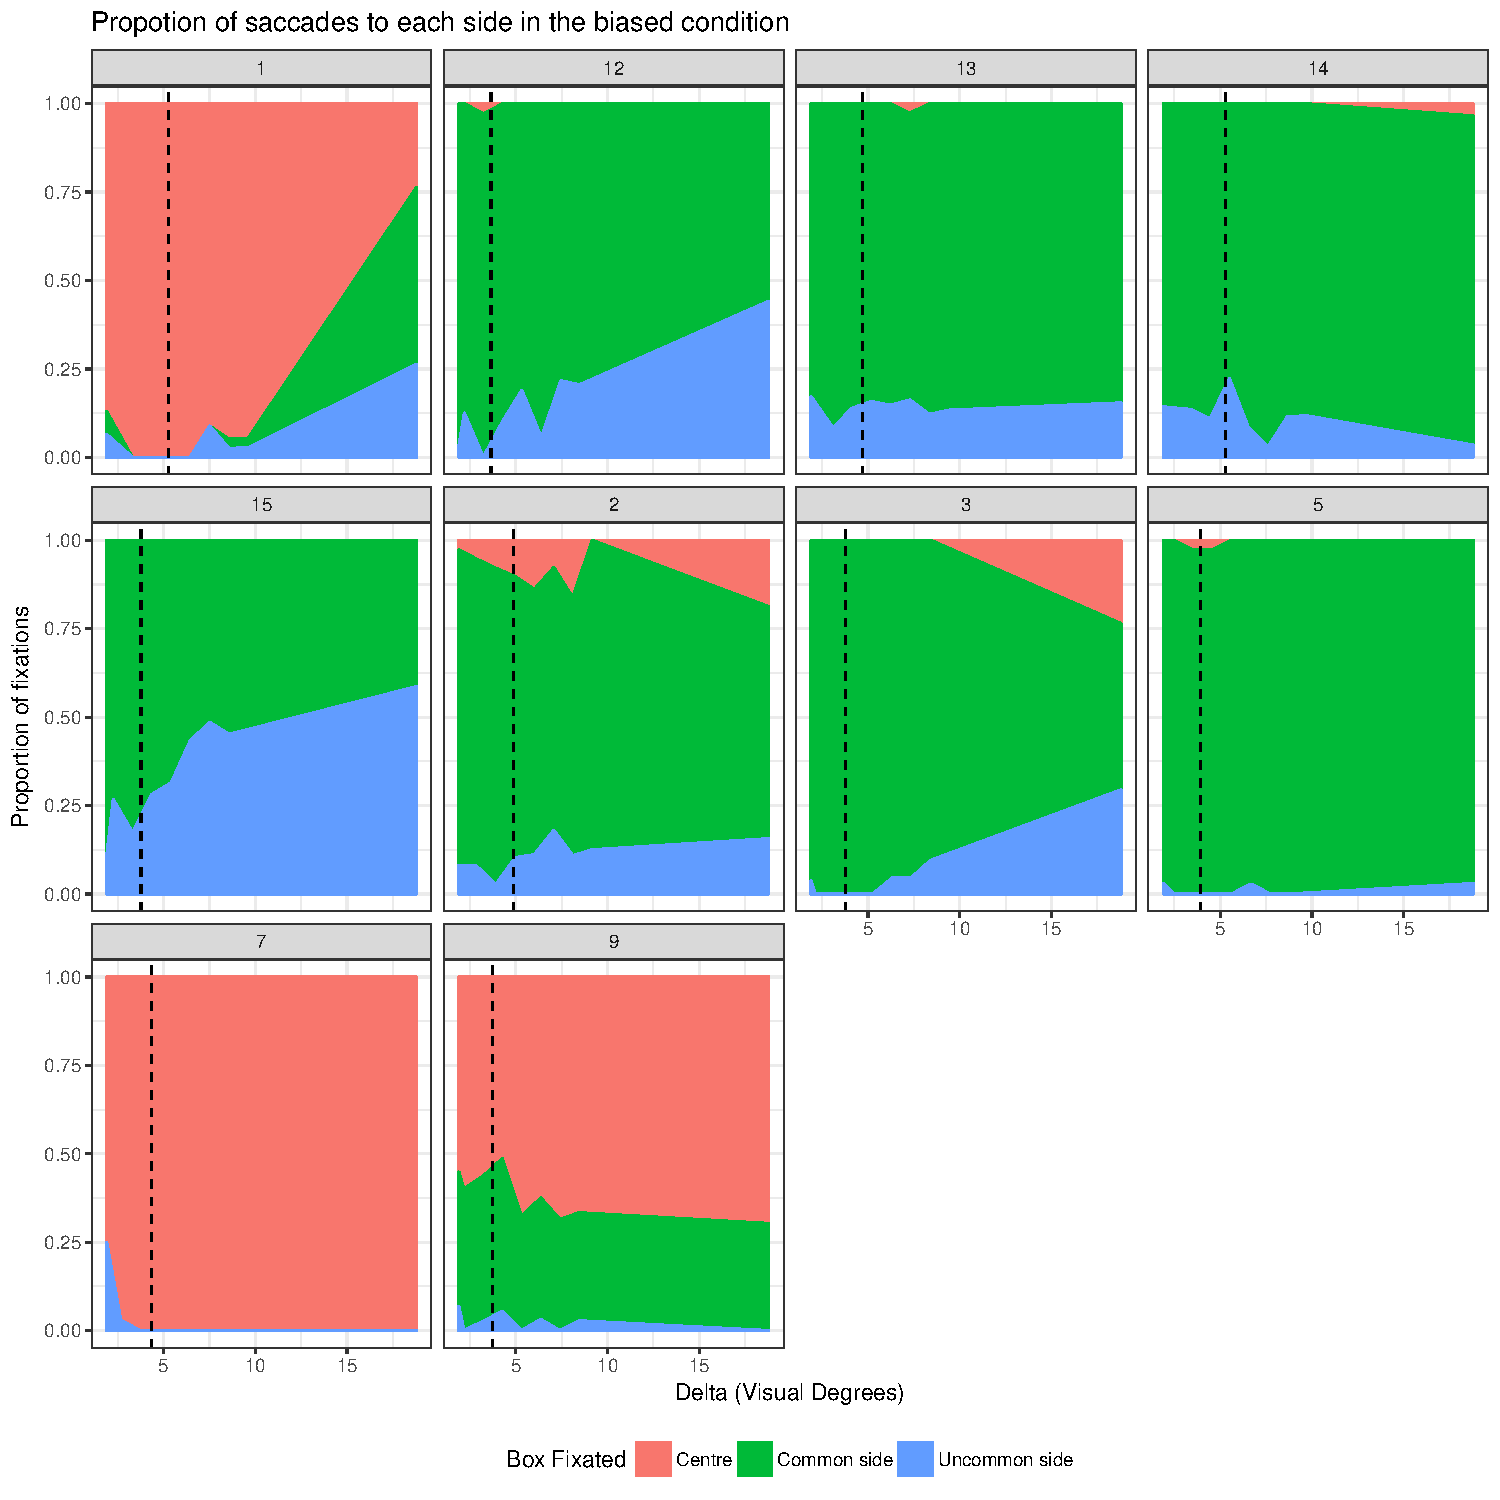
\includegraphics[scale=0.9]{Figures/Experiment_4_prob/Part_2_prop_biased_vdegs}
%	\end{subfigure}
%	\begin{subfigure}
%		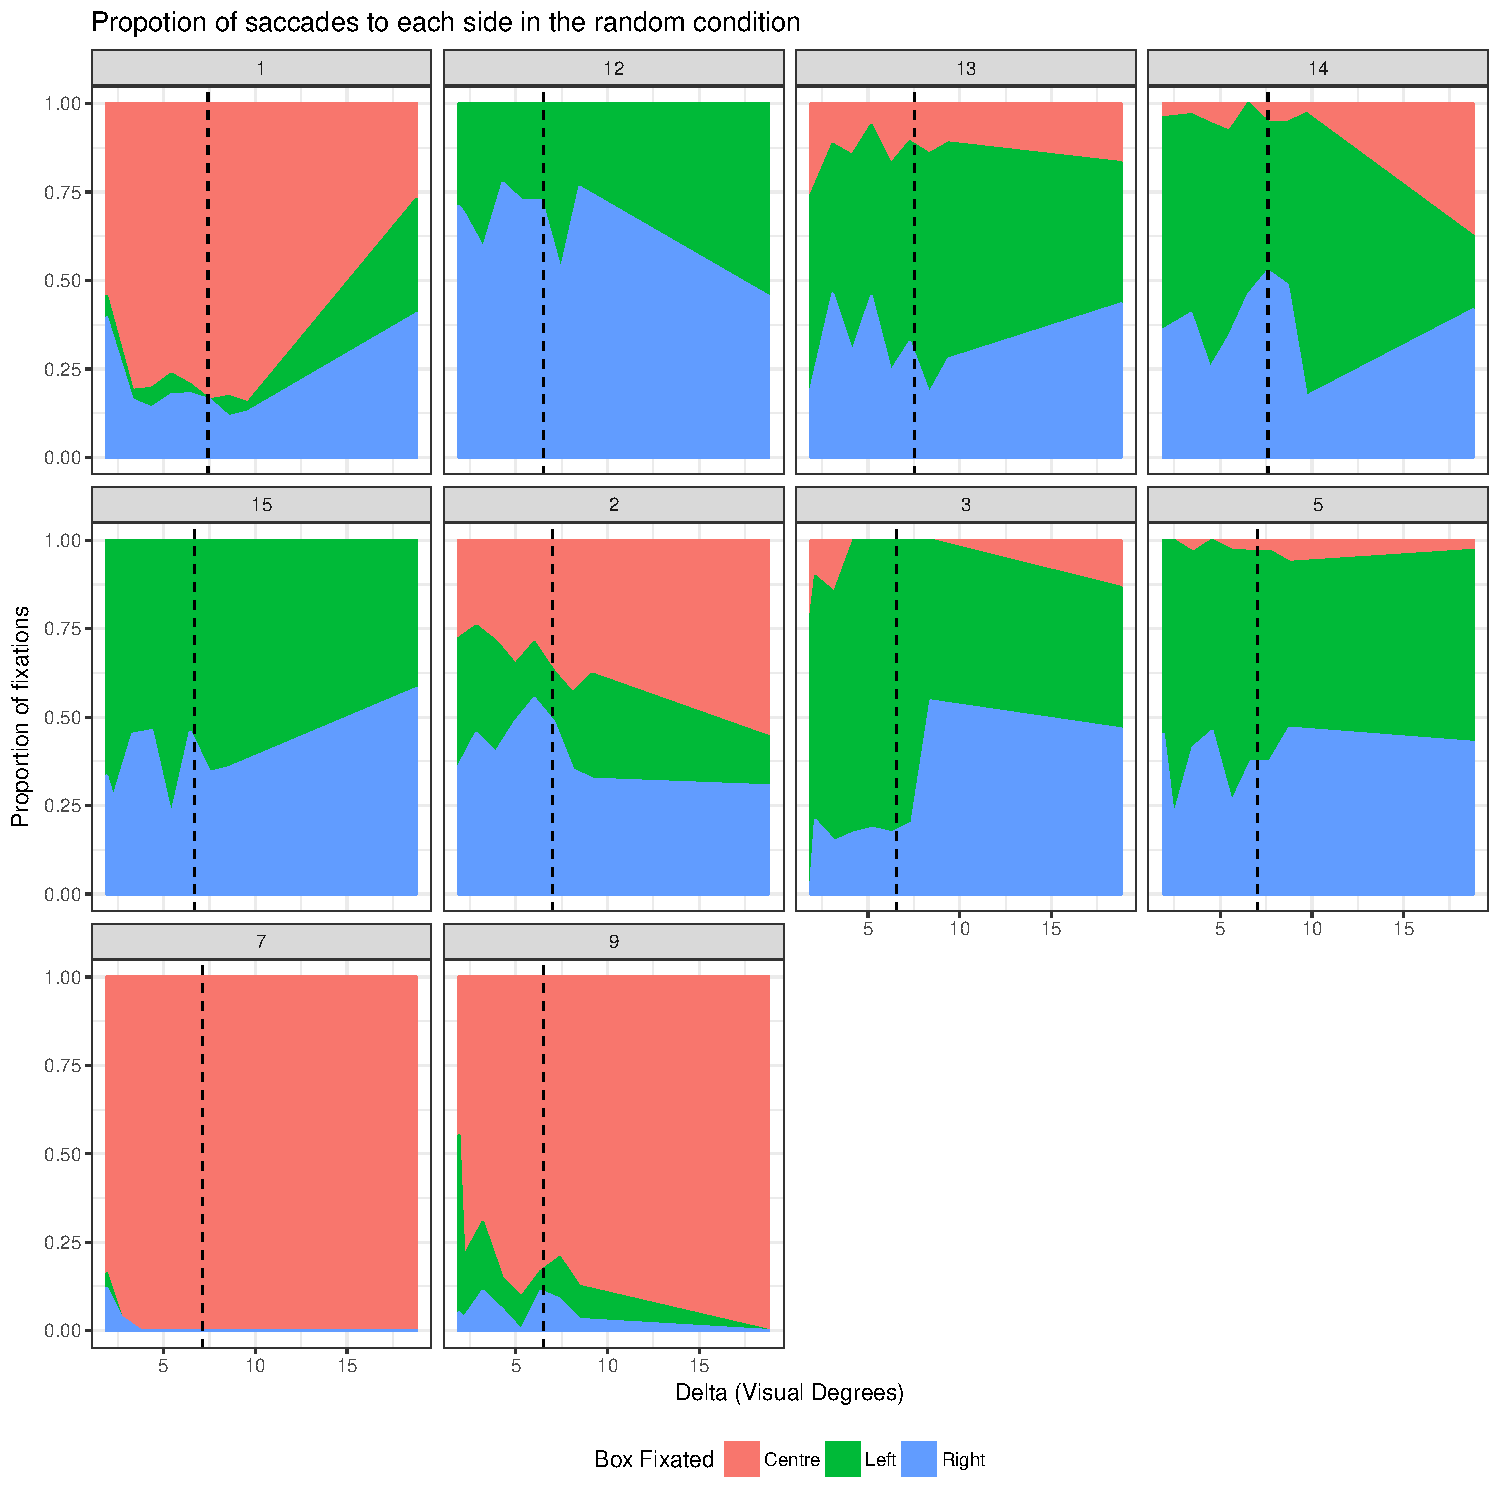
\includegraphics[scale=0.9]{Figures/Experiment_4_prob/Part_2_prop_random_vdegs}
%	\end{subfigure}
%	\caption{The shaded area represents the proportion of fixations made to the box as described by the legends below each plot. Black dotted lines show the switch point for each participant}
%	\label{fig:Session2-prob-props}
%\end{figure}

\begin{figure}
	\centering
	\captionsetup{justification=centering}
	\subfloat{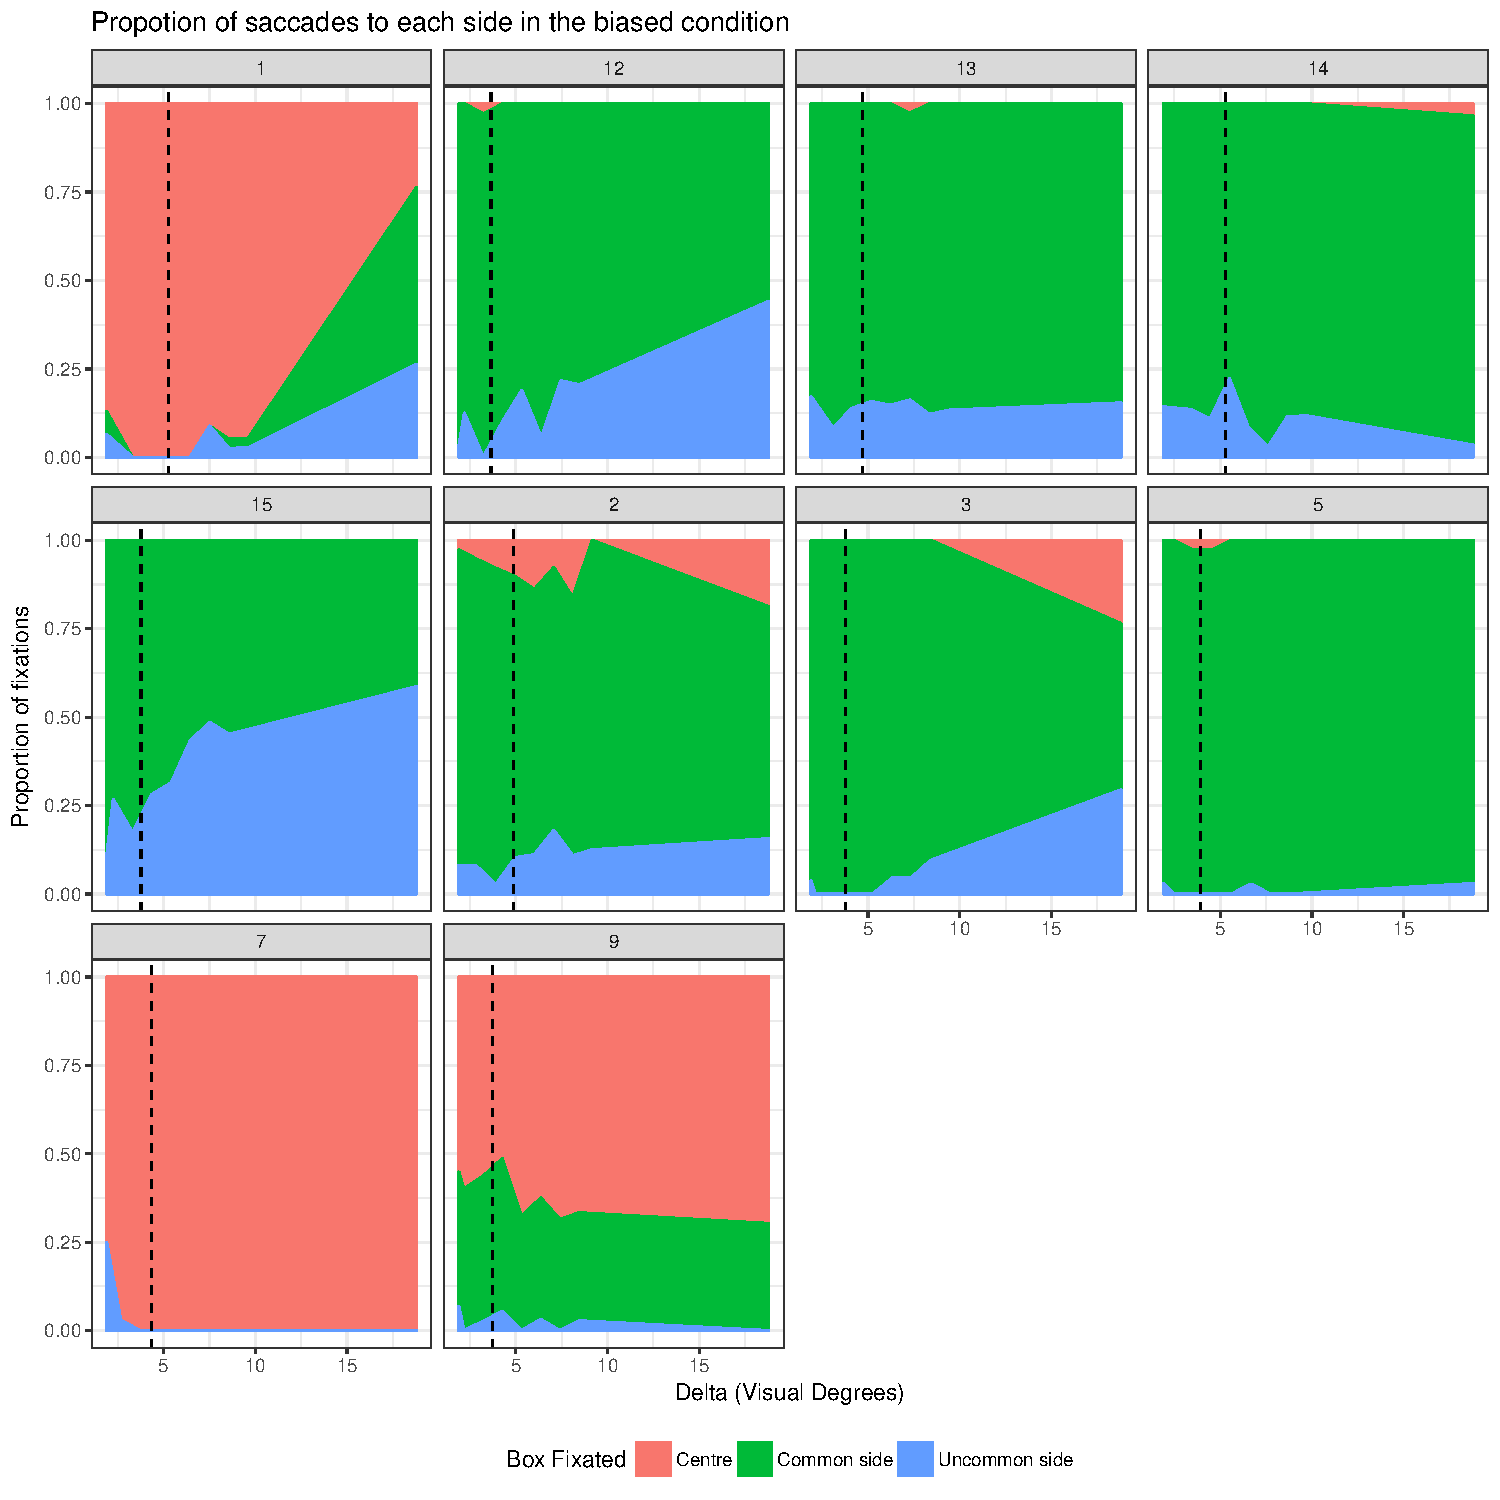
\includegraphics[height = 10cm, width = 15cm]{Figures/Experiment_4_prob/Part_2_prop_biased_vdegs}}\quad
	\subfloat{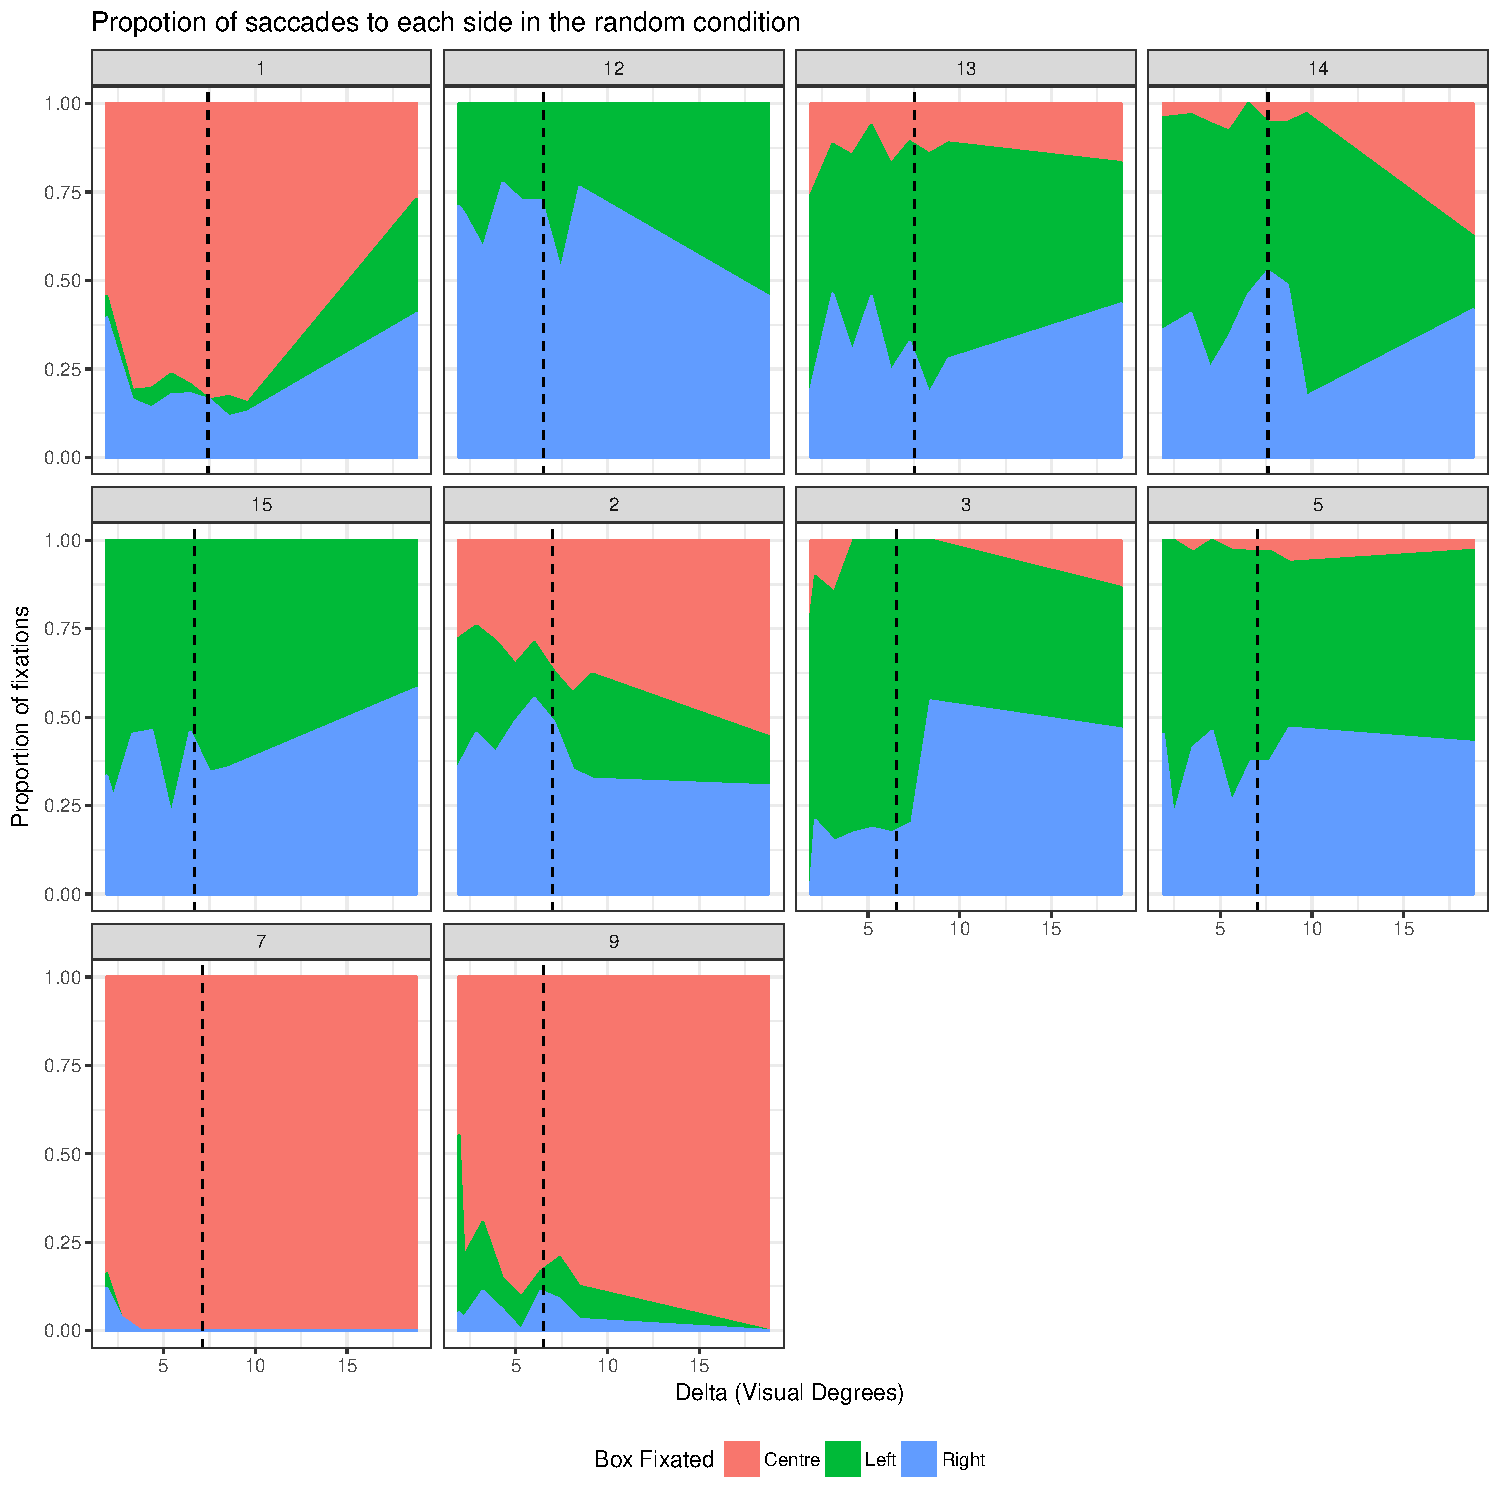
\includegraphics[height=10cm,width=15cm]{Figures/Experiment_4_prob/Part_2_prop_random_vdegs}}
	\caption{The shaded area represents the proportion of fixations made to the box as described by the legends below each plot. Black dotted lines show the switch point for each participant}
	\label{fig:Session2-prob-props}
\end{figure}

%\begin{figure}
%	\centering
%	\captionsetup{justification=centering}
%	\subfloat[][]{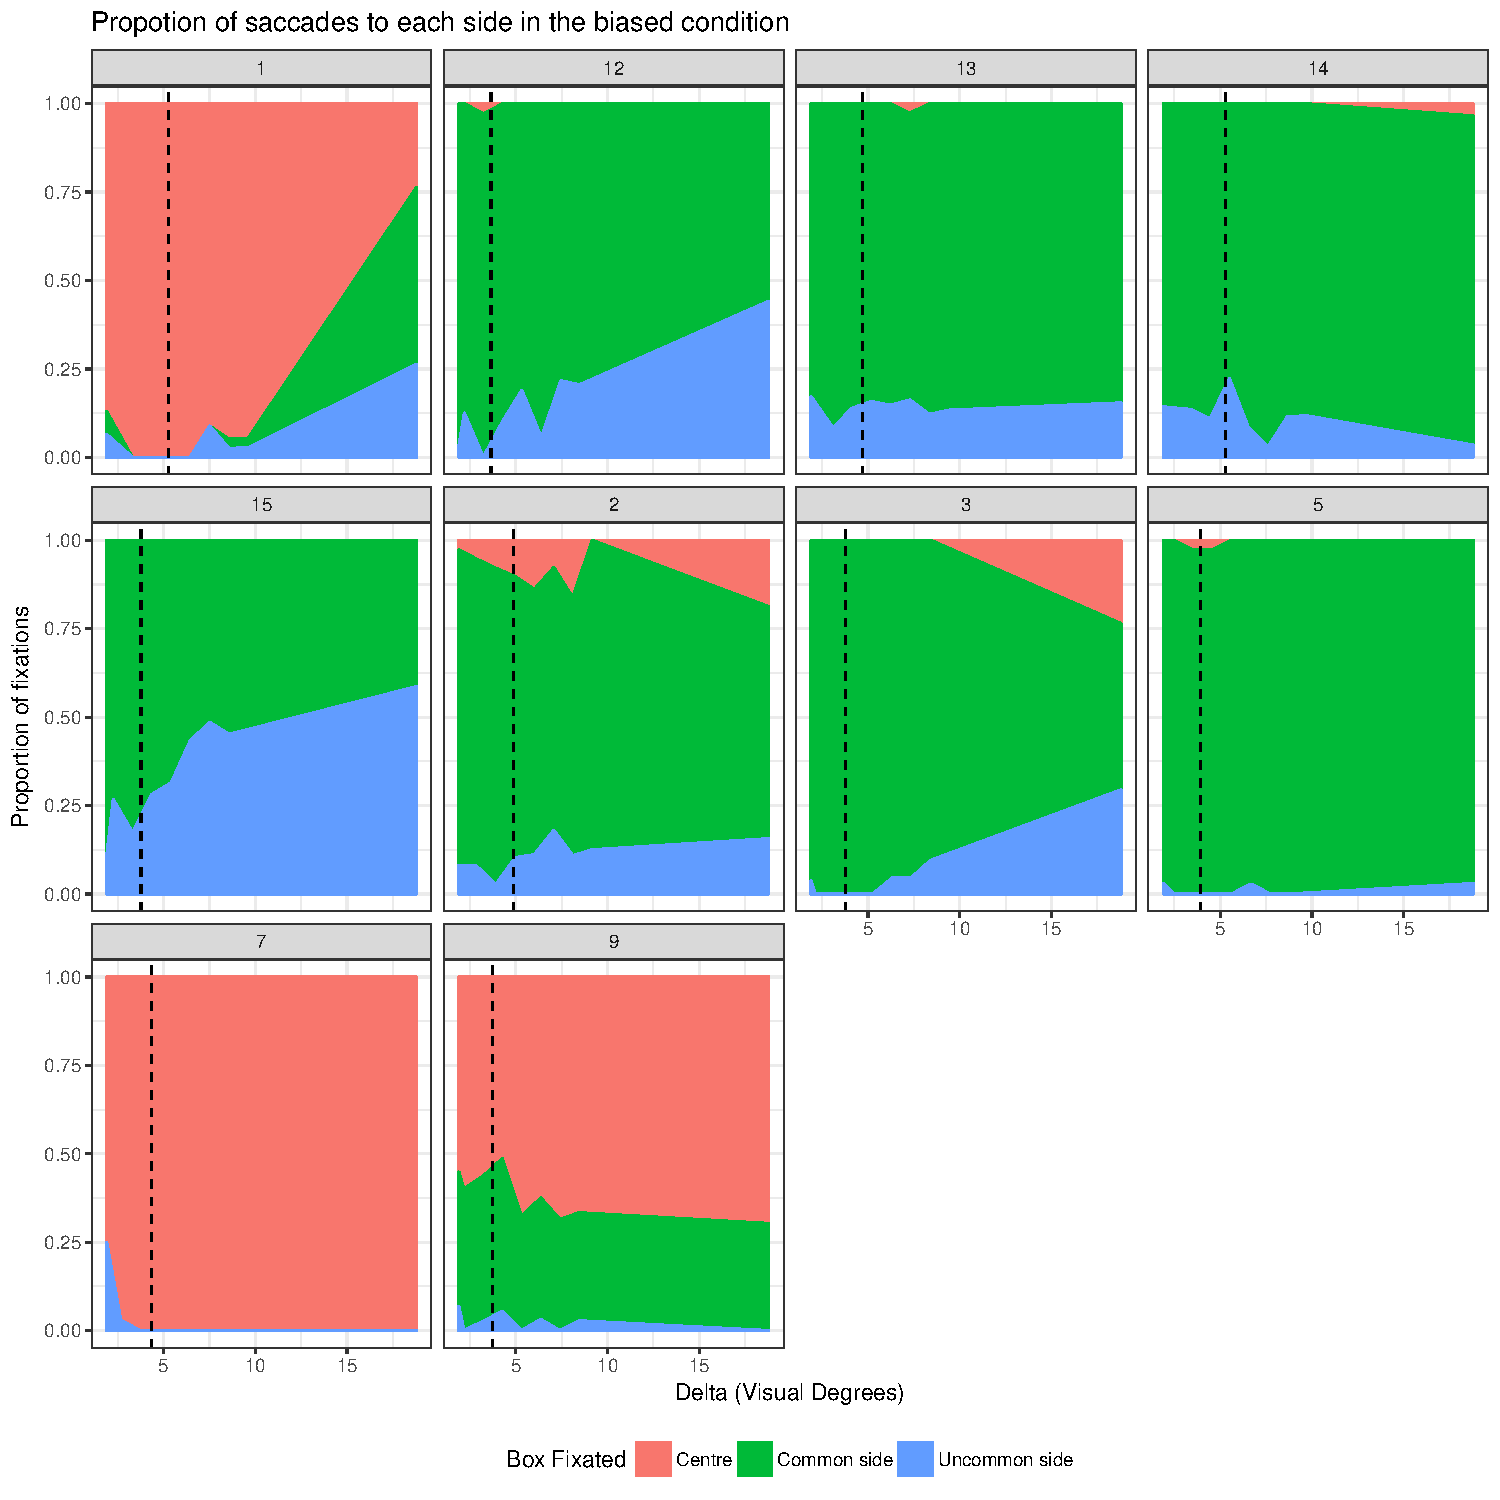
\includegraphics[scale=0.9]{Figures/Experiment_4_prob/Part_2_prop_biased_vdegs}}\\
%	\subfloat[][]{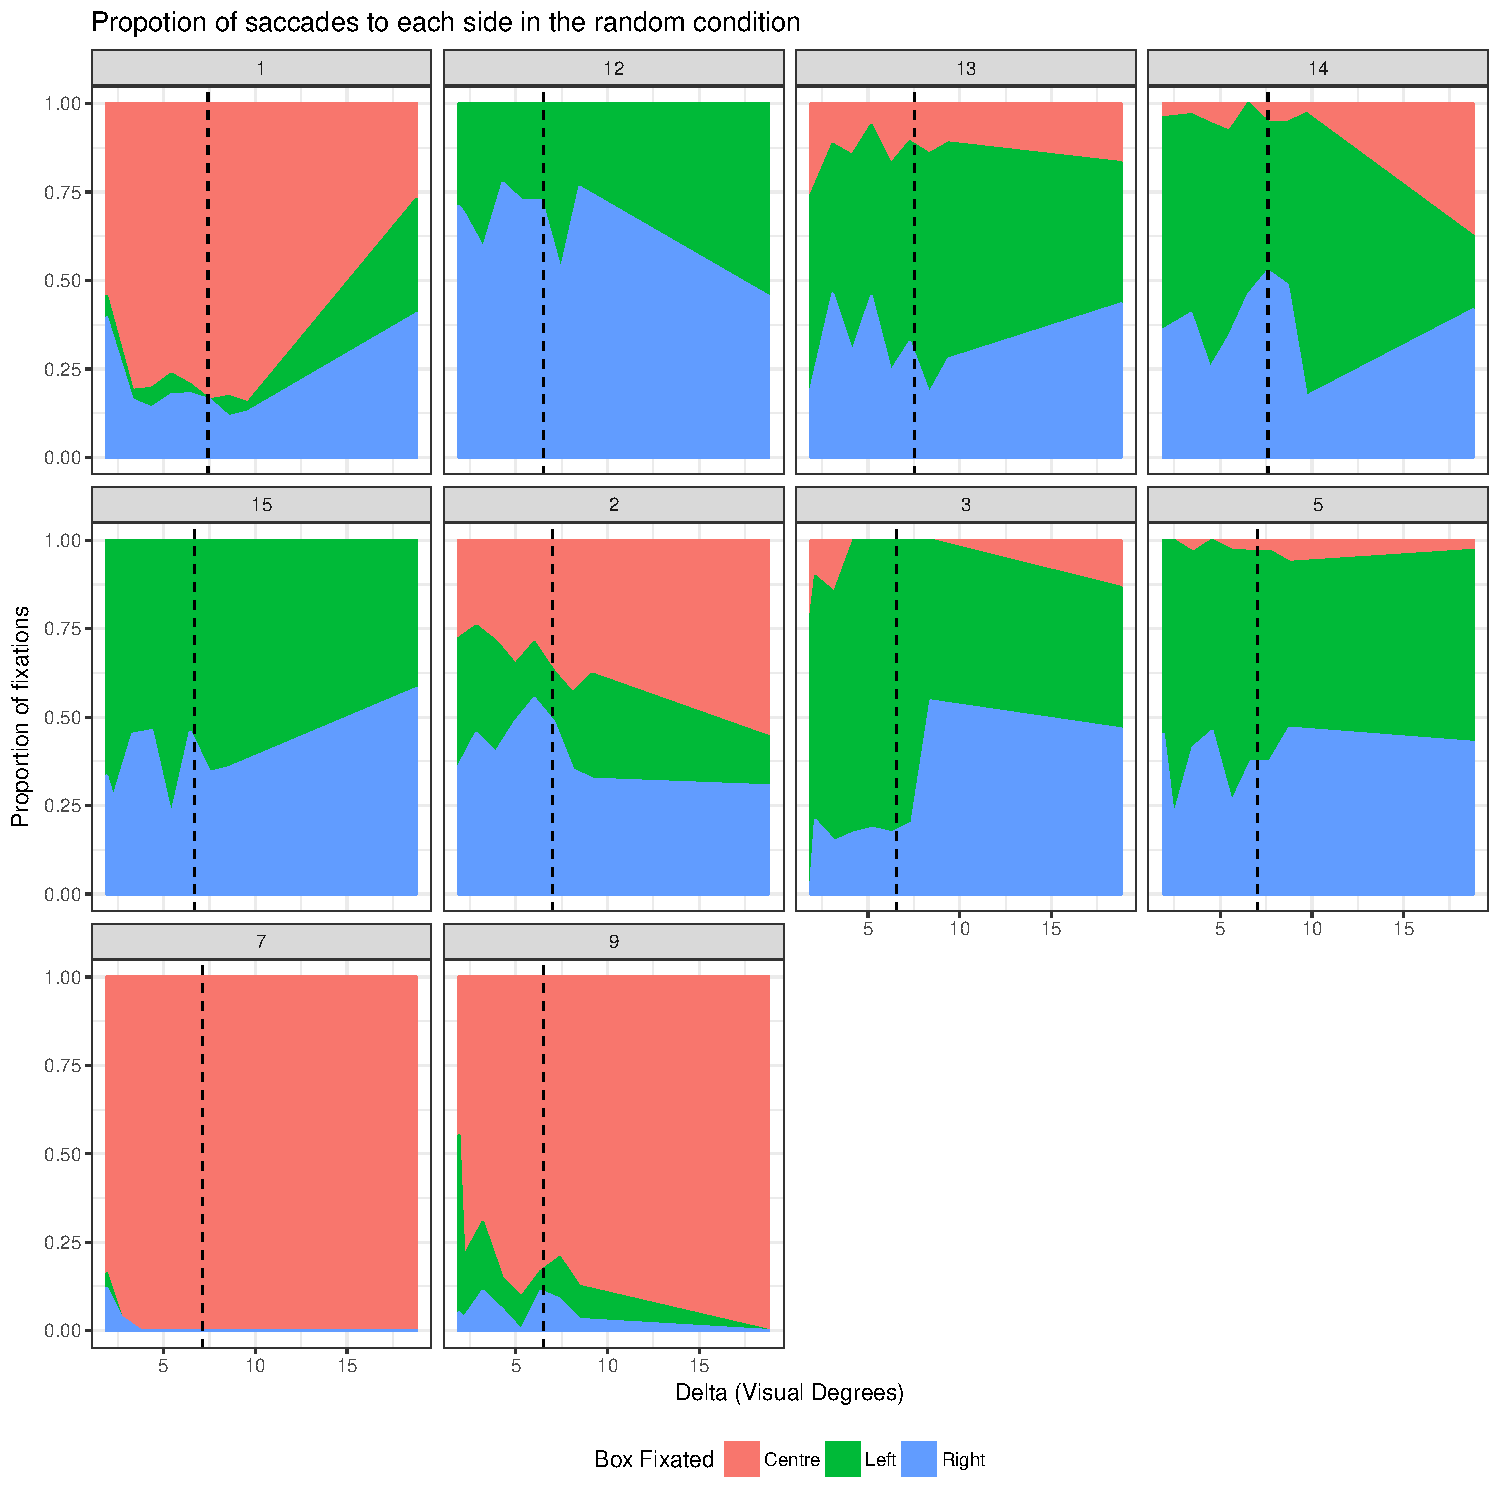
\includegraphics[scale=0.9]{Figures/Experiment_4_prob/Part_2_prop_random_vdegs}}
%	\caption{{The shaded area represents the proportion of fixations made to the box as described by the legends below each plot. Black dotted lines show the switch point for each participant}
%	\label{fig:Session2-prob-props}
%\end{figure}

%\begin{figure}[!ht]
%	\centering
%	\captionsetup{justification=centering}
%	\subfloat[][]{\includegraphics[width=65mm, height = 45mm]{Figures/1,5.jpg}}\quad
%	\subfloat[][]{\includegraphics[width=65mm, height = 45mm]{Figures/2,3.jpg}}\\
%	\subfloat[][]{\includegraphics[width=65mm, height = 45mm]{Figures/3,3.jpg}}\quad
%	\subfloat[][]{\includegraphics[width=65mm, height = 45mm]{Figures/4,3.jpg}}
%	\caption{Some example displays can be seen above. Each display contains a target line tilted 45$^{\circ}$ to the right. a) being the most difficult through to d) being the easiest.}
%	\label{fig:1}
%\end{figure} 


\subsubsection*{Accuracy}
\paragraph{} In order to illustrate how different strategies would lead to different accuracy levels, an estimation of accuracy was calculated based on each participant's pattern of fixations. By doing this, chance is accounted for and therefore if two participants were optimal but one happened to always guess the wrong side and the other always the correct side, they would both have a similar estimated accuracy level. 

\paragraph{} As can be seen in Figure \ref{fig:Session2-prob-accresults}, participant 5 was the only participant that performed in such as way as to reach the optimal expected accuracy. However, this was only in the \textit{Biased} condition. In the \textit{Random} condition, they fixated the side boxes when they should not have which therefore reduced their accuracy to below what would have been expected should they have performed optimally. These plots demonstrate how the different strategies employed by the participants had a direct impact on their performance in the task with the majority falling below the accuracy level that could have been achieved by making use of the optimal strategy. 

\begin{figure}[ht!]
	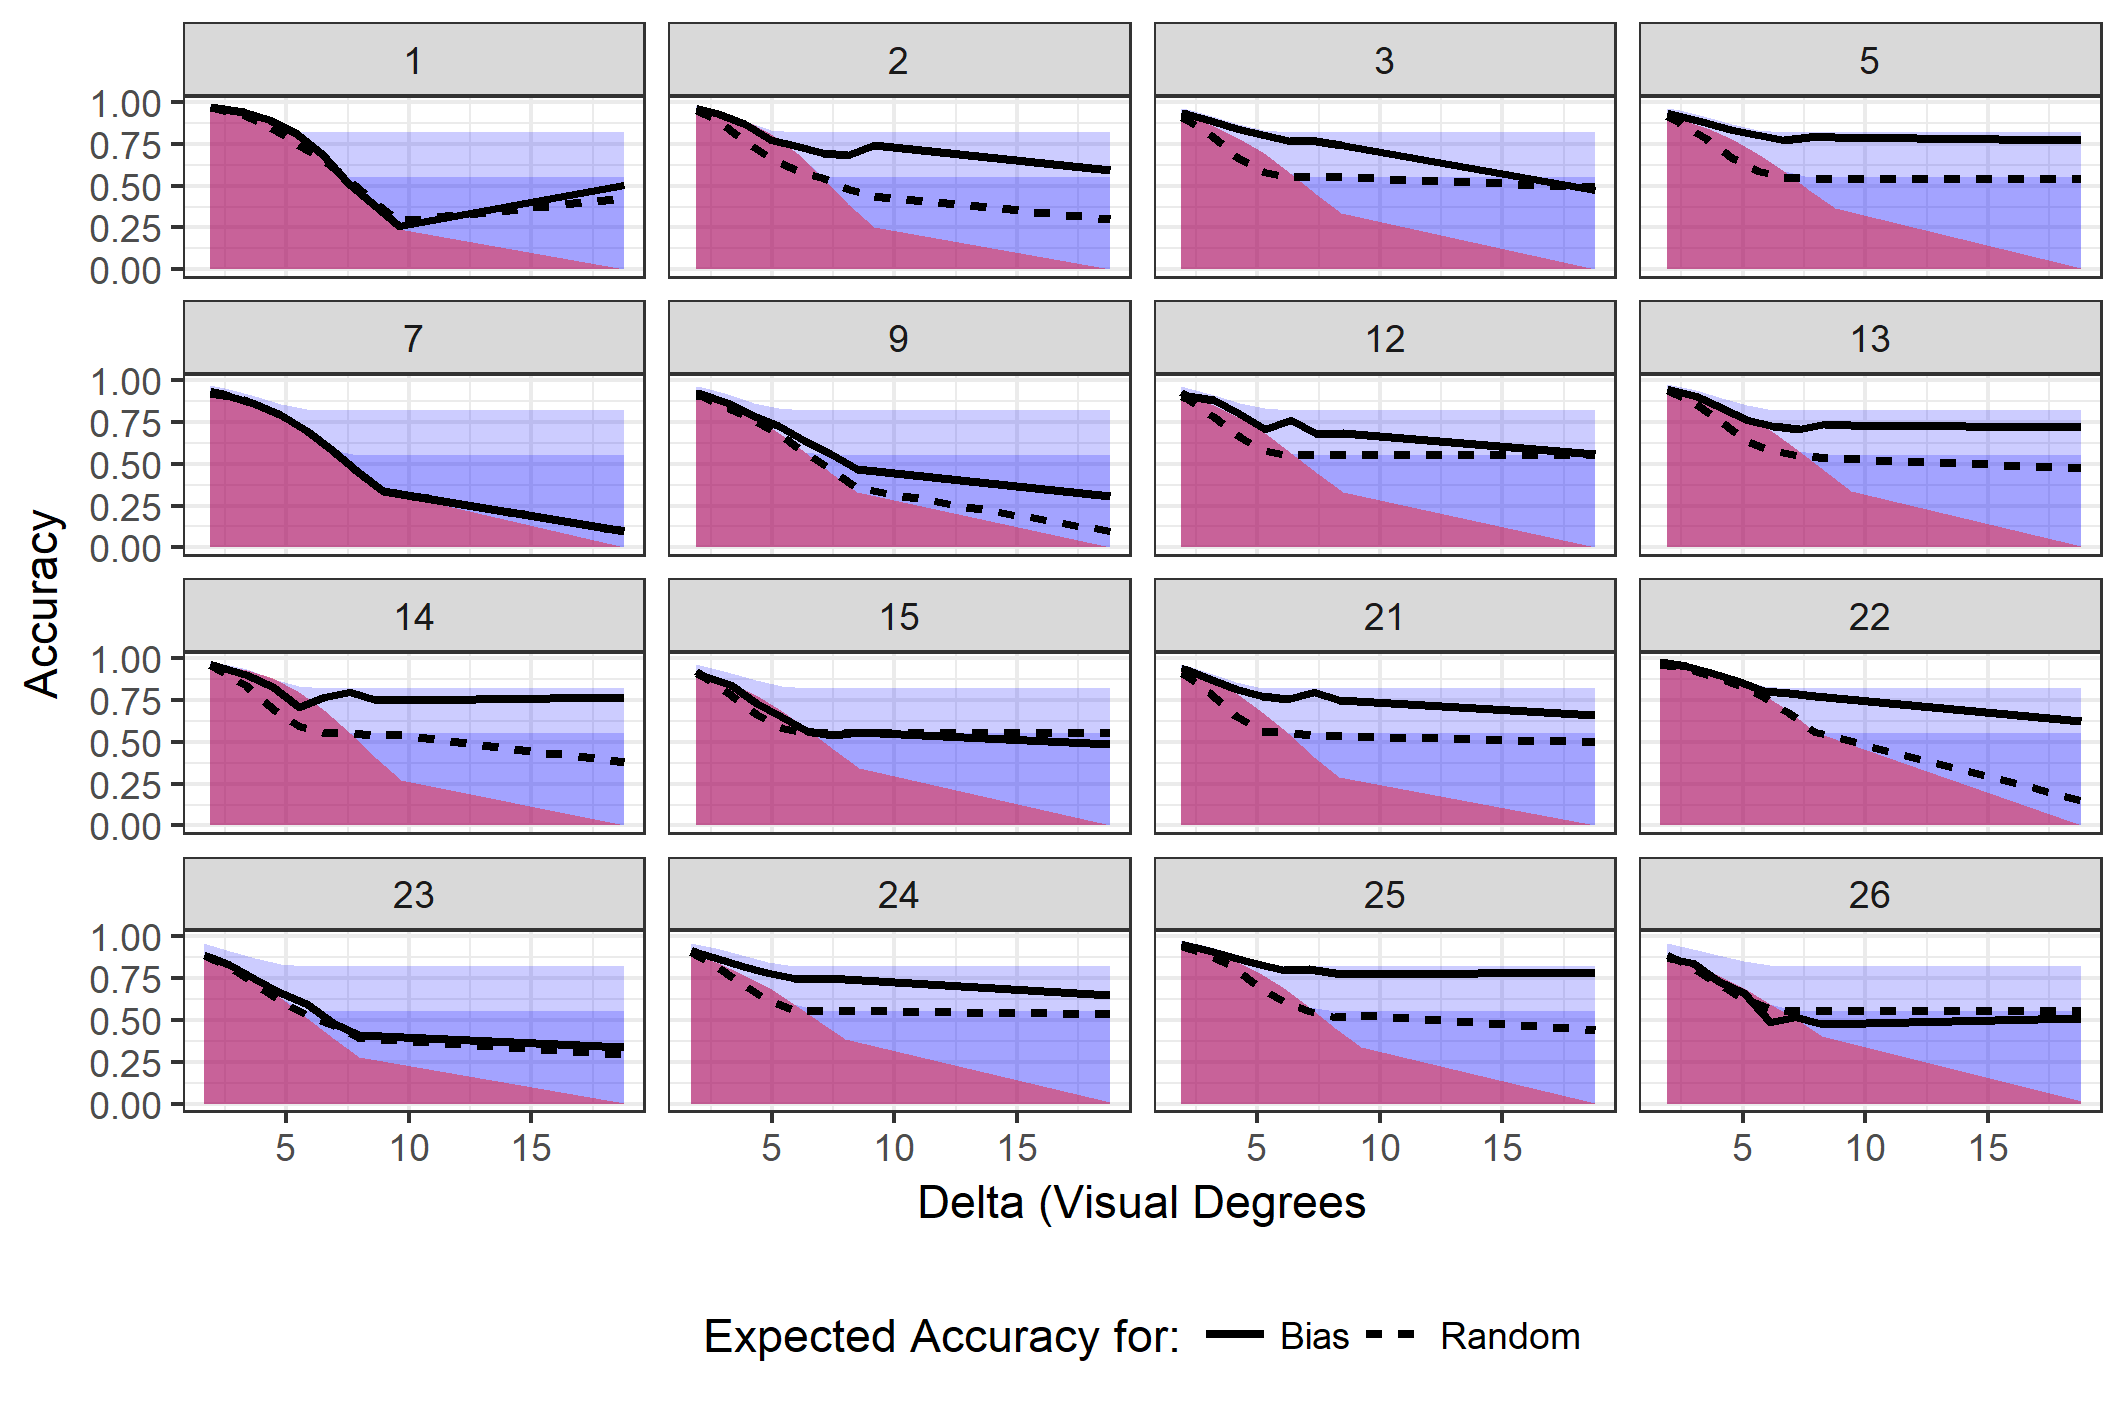
\includegraphics[scale=0.9]{Figures/Experiment_4_prob/Estimated_Accuracy_both}
	\centering
	\captionsetup{justification=centering}
	\caption{These plots show the expected accuracy for each participant given their fixations. The upper limit of the "red" shaded region represents a participants' accuracy should they have exclusively fixated the central box. The upper limit of the darker blue region represents accuracy should the participant have performed optimally in the \textit{Random} condition. The lighter region is the same again, but for the \textit{Biased} condition}
	\label{fig:Session2-prob-accresults}
\end{figure}

\subsection*{Discussion}
\addcontentsline{toc}{subsection}{Discussion}
\paragraph{} Although preliminary, these results suggest that simply adding a bias for one side to contain the target more often does not facilitate the use of the optimal strategy. This would suggest that it is unlikely that participants were unable to employ the optimal strategy simply because they could not decide which target to prioritise. These results are in line with what has been discussed above with relation to probability matching. Only one participant displayed maximising behaviour with the rest of the participants choosing to attempt to fixate each box with respect to the underlying probably as stated prior to each block. The average amount of fixations to the common target in the \textit{Biased} condition was 85\%. This is close to what the actual percentage was for this condition and is close to the idea of Probability Matching \citep{Koehler2010}. With this in mind, it's possible that participants thought less about their visual acuity and more about the underlying chance of success attached to picking each option. It would be interesting to investigate whether not telling participants the underlying proportions would result in the same sort of behaviour. Although it has been suggested that probability matching occurs even when participants are not explicitly told about the probability of each event happening \citep{Gao2015}, within the context of this task it may make a difference. Informing participants about this information may cause them to prioritise its use over accounting for their performance.

%\newpage
\section*{Experiment 2: Altering Hoop Sizes}
\addcontentsline{toc}{section}{Experiment 2: Altering Hoop Sizes}

\subsection*{Preface}
\addcontentsline{toc}{subsection}{Preface}
\paragraph{} In \textit{Experiment 1}, participants were tasked with recognising two fairly abstract concepts; they were to estimate their own visual acuity, and understand probability (and potentially track this depending on how valid they believed the information to be). As such, these abstract concepts may have been difficult for participants to make use of when making their decisions. As such, for \textit{Experiments 2 \& 3}, the \textit{Throwing Task} as described in \cite{clarke2015failure} was used when investigating the other potential influences. This was also decided due to practical reasons as it would be difficult to alter the \textit{Detection Task} in such a way to test the influence of the factors being investigated in \textit{Experiments 2 \& 3}. 

\paragraph{} The results of \textit{Experiment 1} suggested that even though participants made use of probability information, they were still unable to account for their own ability to perform and thus reach an accuracy level that would have been expected given the optimal strategy had been used. However, as participants rarely appeared to opt for the \textit{maximising} strategy, this would indicate a reluctance to commit entirely to one option or the other. In \textit{Experiment 2} we aimed to investigate this further by altering the \textit{Throwing Task} \citep{clarke2015failure} so that it would be easier to achieve the goal should it appear on one side if they were to stand equidistant from each target. This was carried out to investigate whether it was the case that participants were attempting to make use of a strategy that avoided a sure loss. As such, if participants were attempting this, they should stand closer to the more difficult target as this would equalise their chances of success. 
 
 
 %\paragraph{} For \textit{Experiment 2}, the aim was to investigate whether participants were attempting to give themselves and equal chance at achieving each target regardless of which would become the target, much like in \cite{CHAPMAN2010168}. To do this, the relative difficulty of succeeding at each target was altered so that one side would be easier than the other should the participant position their self equidistant from both potential targets. However, if the participants were trying to give themselves and equal chance of success, they should have stood more closely to the more difficult target in order to equate their ability to succeed at both targets. 
 
\subsection*{Methods}
\addcontentsline{toc}{subsection}{Methods}
\subsubsection*{Participants}
\paragraph{} In total, 21 participants (4 male) took part in this experiment, with an average age of 21 (\textit{SD} = 0.92). Participants were recruited via word of mouth.

\subsubsection*{Procedure}
%GET measurements of the hoops that were used.
\paragraph{} The experiment took place over two separate sessions with at least one week between the first and second part of the experiment. The experiment was conducted in a sheltered, and paved area of the University of Aberdeen. The paving slabs acted as a convenient metric by which to judge participant standing position and the placement of hoops. The paving slabs measured $0.46cm \times 0.61cm$.

\paragraph{} In Session 1, participants threw 12 bean bags into a series of hoops placed at seven distances from a central location in two different directions. For this experiment, there were two hoop sizes which had a diameter of $63.5cm$ for the \textit{Large hoops} and the \textit{small hoops} had a diameter of $35.5cm$. This was carried out in two different directions (hereby referred to as North and South) with the starting direction counterbalanced across participants. This meant that for each distance, the participant produced an accuracy score of \textit{x} out of 24 which was then used to model how the participant's accuracy decreased as a function of distance. The Large hoops were tested at a set of distances that were larger (from 7 slabs/$3.22m$ to 25 slabs/$11.5m$) than that of the small hoops (from 3 slabs/$1.38m$ to 19 slabs/$8.74$) so as to get an accurate measure of where the participant's accuracy dropped to an appropriate level for the design (see Figure \ref{fig:Session1-Throwing}). The results of the Session 1 can be seen in Figure \ref{fig:Session1-HoopSizes}.

%NOTE 
% These figures have different x-axes... so you should update that as soon as
% This is still pretty horrible... but it should be messed about with once everything above it sorted out...
% Will need to mess around with this a fair bit as we go
\begin{figure}[ht!]%{l}{0.5\textwidth}%[ht!]
	\begin{center}
		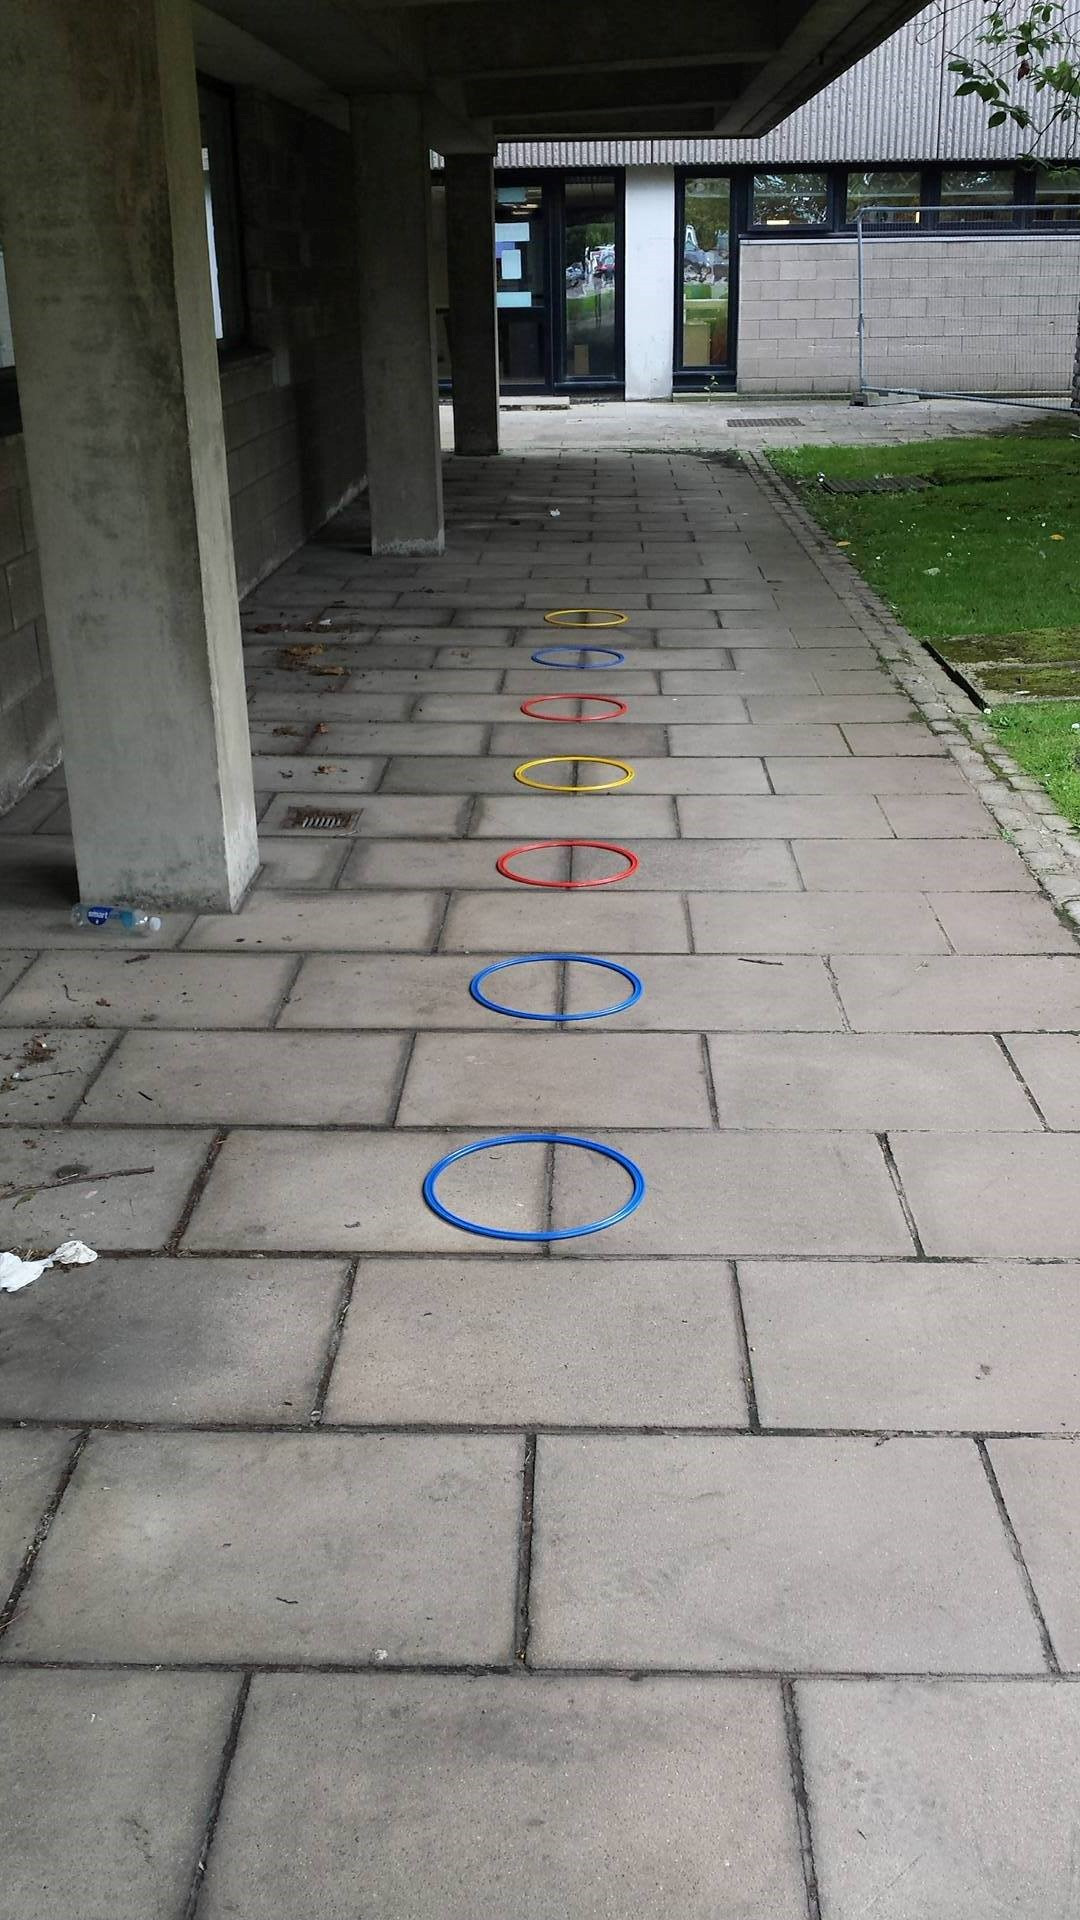
\includegraphics[scale=0.25]{Figures/Experiment_1_Awareness/Layout_part1}
		%\centering
		\captionsetup{justification=centering}
		\caption{This shows the set up for session 1 from the participant's point of view.}
		%\vspace{-50pt}
		\label{fig:Session1-Throwing}
	\end{center}
\end{figure}

\paragraph{} Using the information collected in Session 1, we were able to calculate the distances at which participants were 10\%, 50\%, and 90\% accurate for both hoop sizes. In order to get one set of distances, a general linear model was fit to each participant's individual accuracy for both hoop sizes separately, then the distances that were calculated for the point at which they were 10\%, 50\%, and 90\% accurate were averaged together. For example, if they were 50\% accurate up to 10 slabs for the large hoops up to eight for the small hoops, the hoops would both be placed 9 slabs from the centre point. This way the experiment was tailored to each individual's ability to accurately throw the bean bags into the hoops at different distances. These distances were then used to decide where the hoops were to be placed in Session 2. In this session, six hoops with 3 pairs defined by their colour were placed on the paved area (see Figure \ref{fig:Session2-Throwing} for the arrangement). Unbeknownst to the participant, each colour pair corresponded to one of the accuracy levels mentioned above (Red = 90\%, Yellow = 50\%, Blue = 10\%) as measured from an unmarked central position, equidistant from both hoops. A second set of distances were also derived from these by subtracting 1, adding 1, and adding 2 "slabs" to the distancethat corresponded to 50\% accuracy.

\begin{figure}[ht!]
	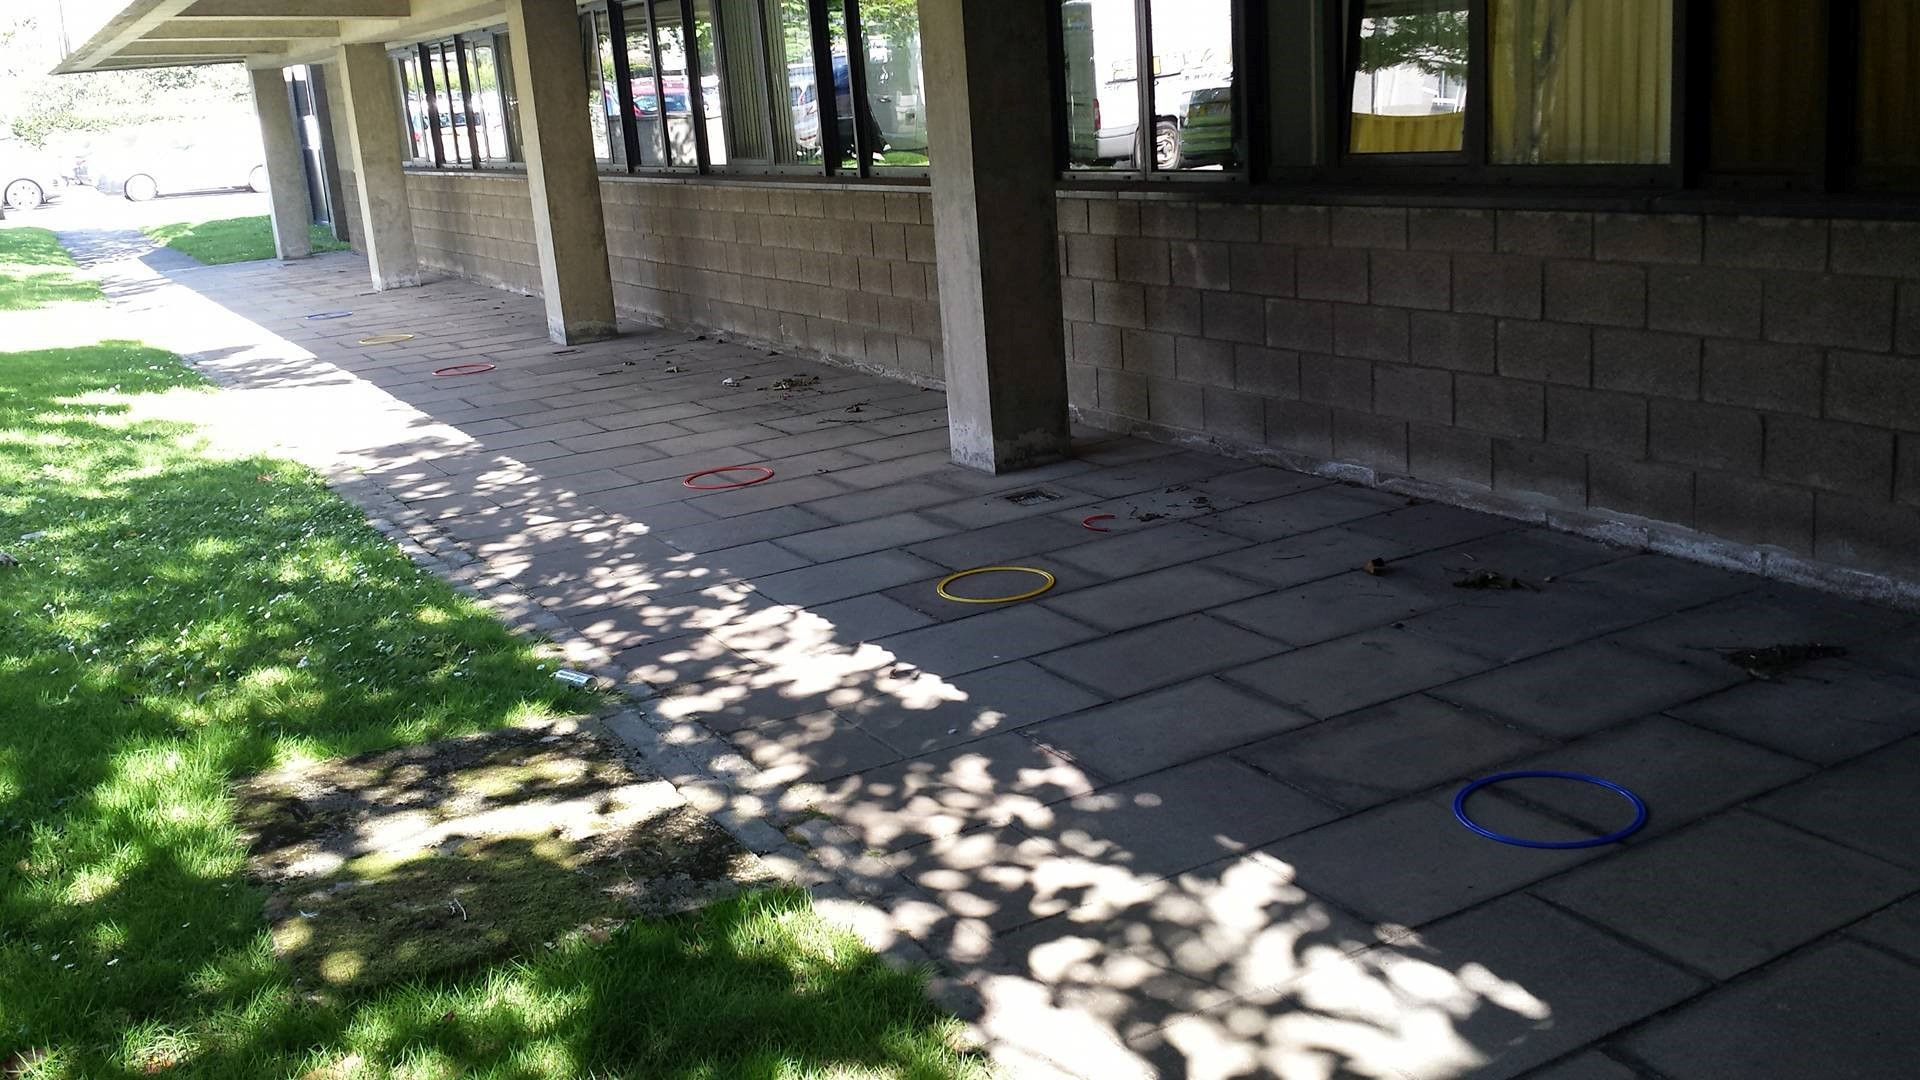
\includegraphics[scale=0.33]{Figures/Experiment_1_Awareness/Layout_part2}
	\centering
	\captionsetup{justification=centering}
	\caption{The setup for session 2}
	\label{fig:Session2-Throwing}
	\vspace{-0.5cm}
\end{figure}

\begin{figure}[ht!]
	%[height = 10cm, width = 16cm] seems to look a bit squashed
	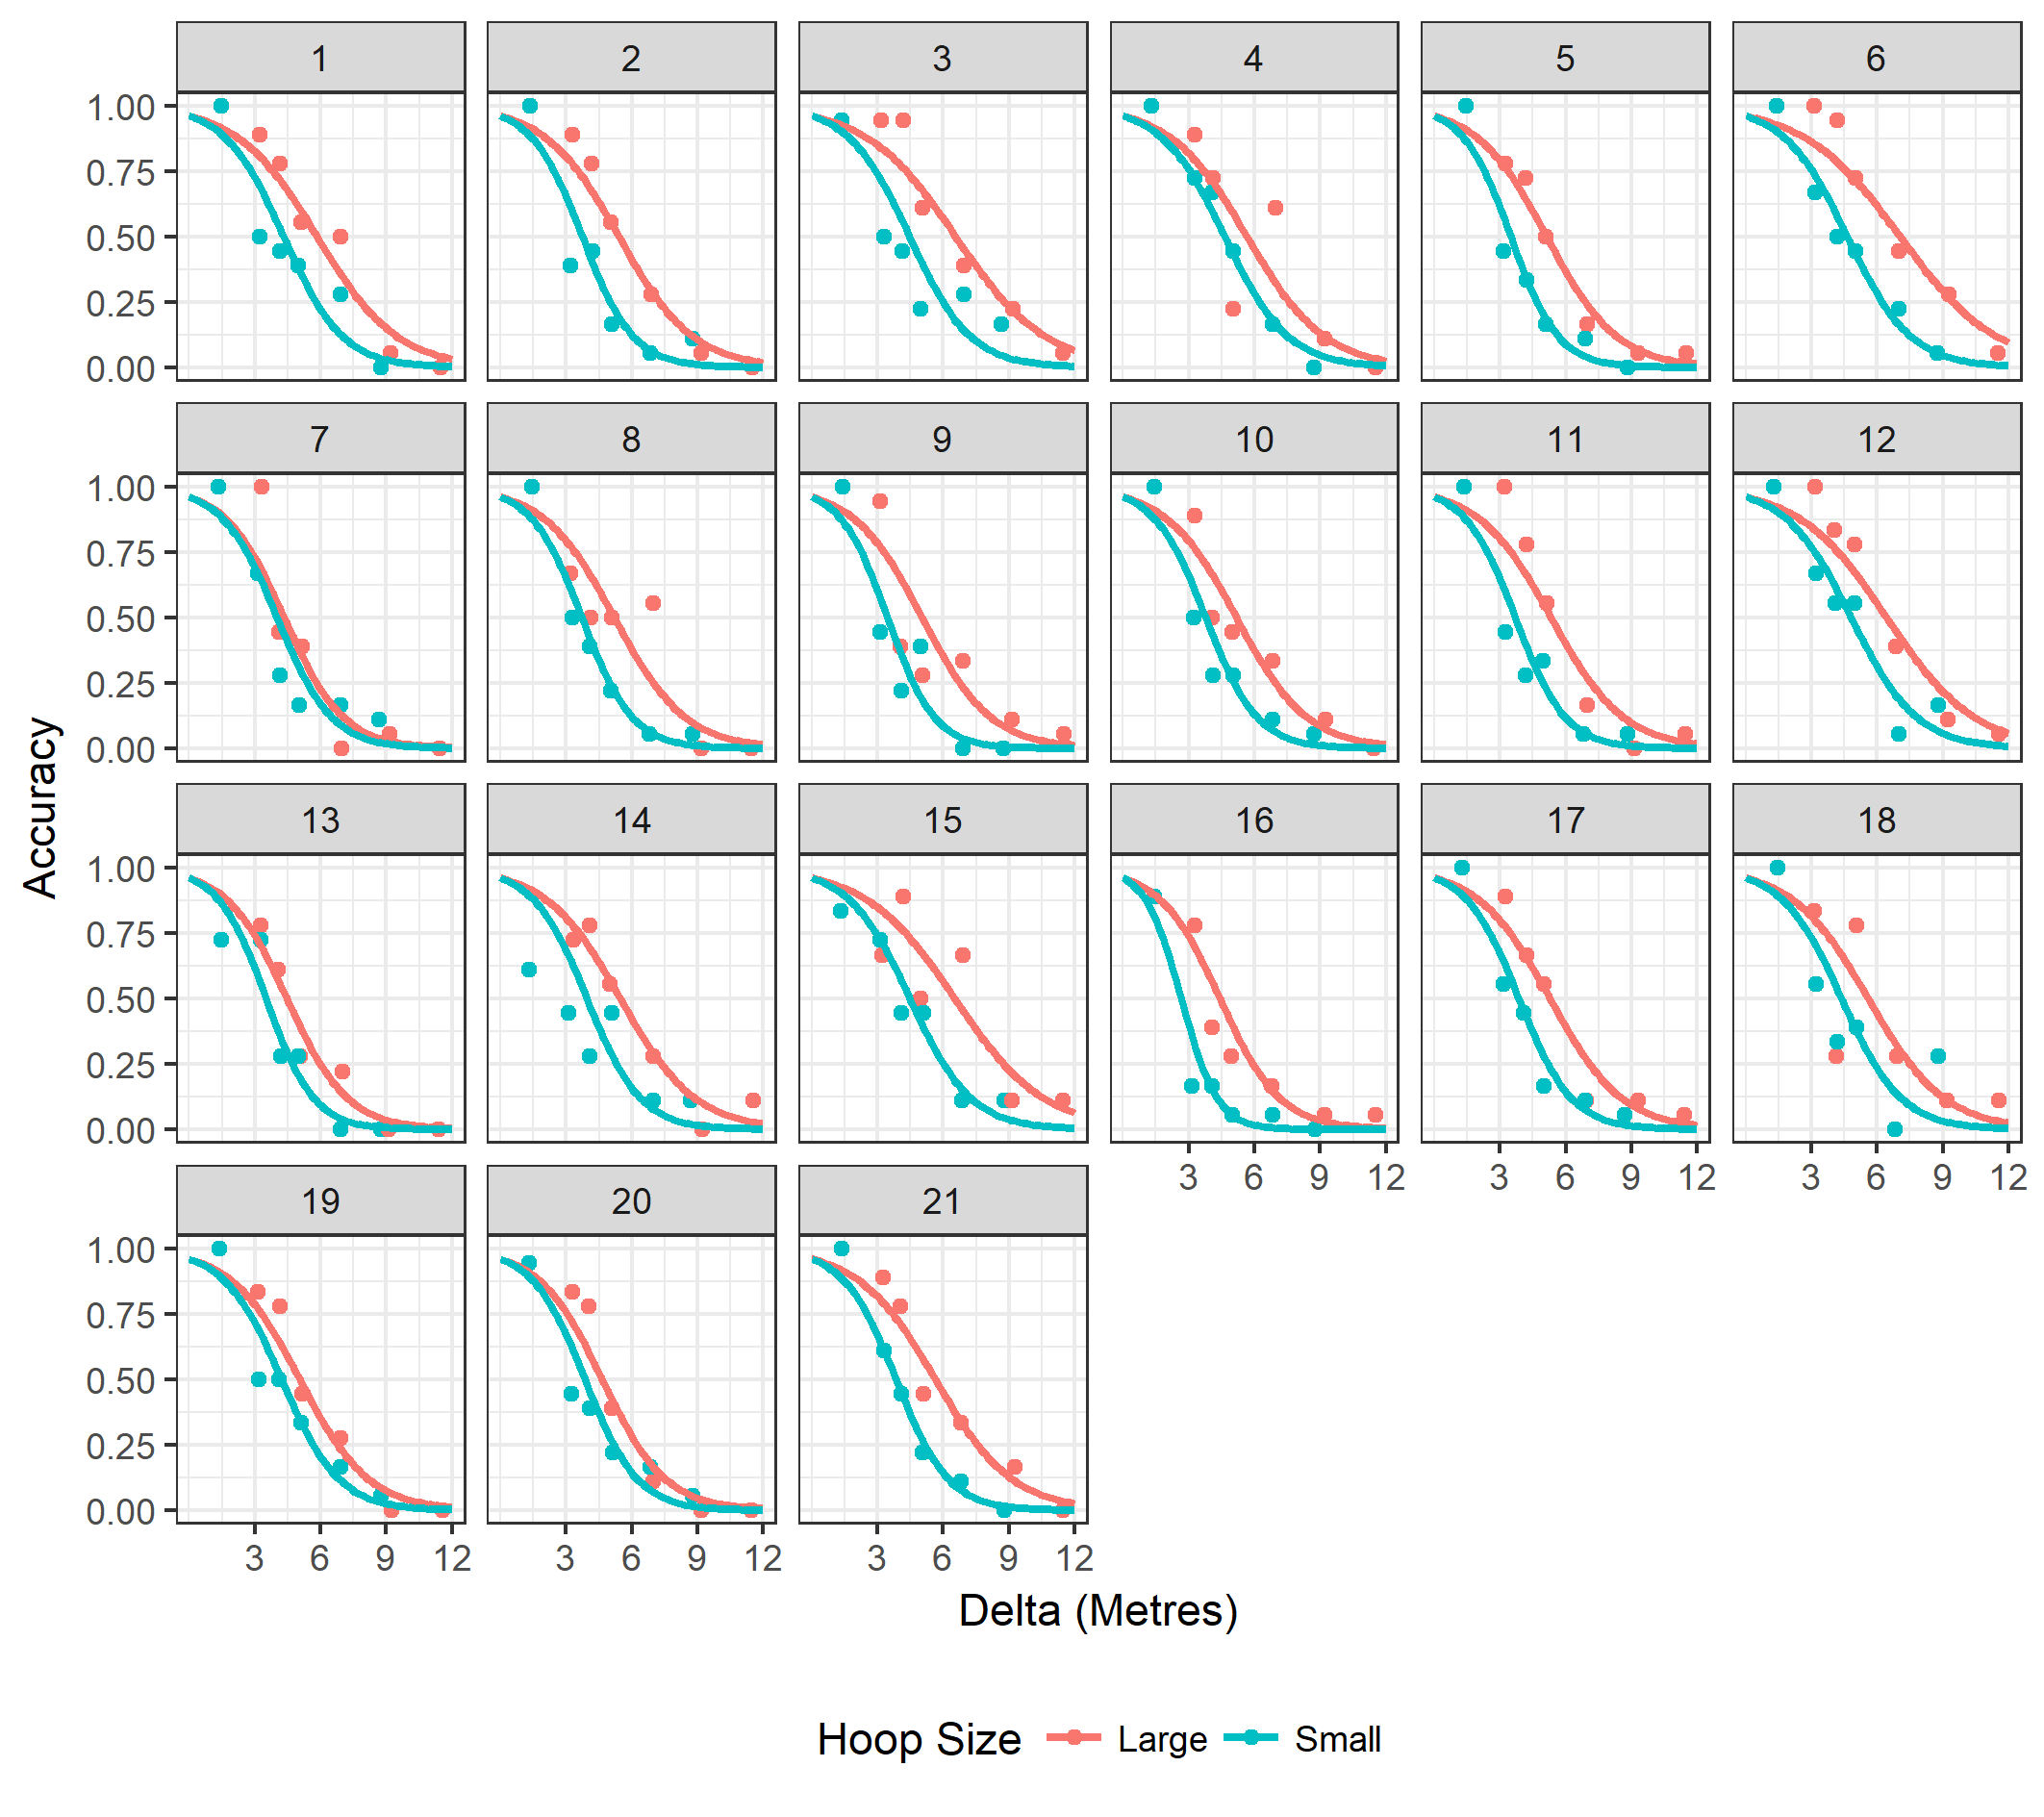
\includegraphics[scale= 0.9]{Figures/Experiment_3_Hoop_size/Session_1_plot}
	\centering
	\captionsetup{justification=centering}
	\caption{These graphs show the binomial regression curves fit to participants' data for Session 1. For the majority participants, it's clear that there is a difference in accuracy for each hoop size.}
	\label{fig:Session1-HoopSizes}
	%\vspace{-0.5cm}
\end{figure}

\paragraph{} In Session 2, participants would draw one bean bag from a bag that contained nine beanbags with three of each colour (Red, Yellow, and Blue). Once thrown, these would be set aside until all nine had been removed from the bag at which point they were replaced. The bag was set off to the side of the paved area so all participants were essentially \textit{"reset"} before each trial. The colour of the bean bag indicated the pair of hoops that would contain the target for that trial. However, participants were told that they would not be informed as to which hoop was the target until they had selected somewhere to stand. They were told they were allowed to stand anywhere they wanted on the paved area and that the target hoop had been predetermined in a random fashion so each hoop was equally likely on every trial. Once participants had selected somewhere to stand and informed the experimenter, their position was recorded and they were told whether they were to aim for the North or South hoop. As mentioned above, the central point of this setup would not yield and equal chance to succeed at both hoops. The position that participants would have to stand in order to maintain an equal chance of success was shifted slightly towards the smaller hoop. The location of each hoop (i.e. the small and the large) was mixed so that not all of the small hoops were on one side for any participant. 

\subsection*{Results}
\addcontentsline{toc}{subsection}{Results}

\subsubsection*{Standing Position}
\begin{figure}[ht!]
	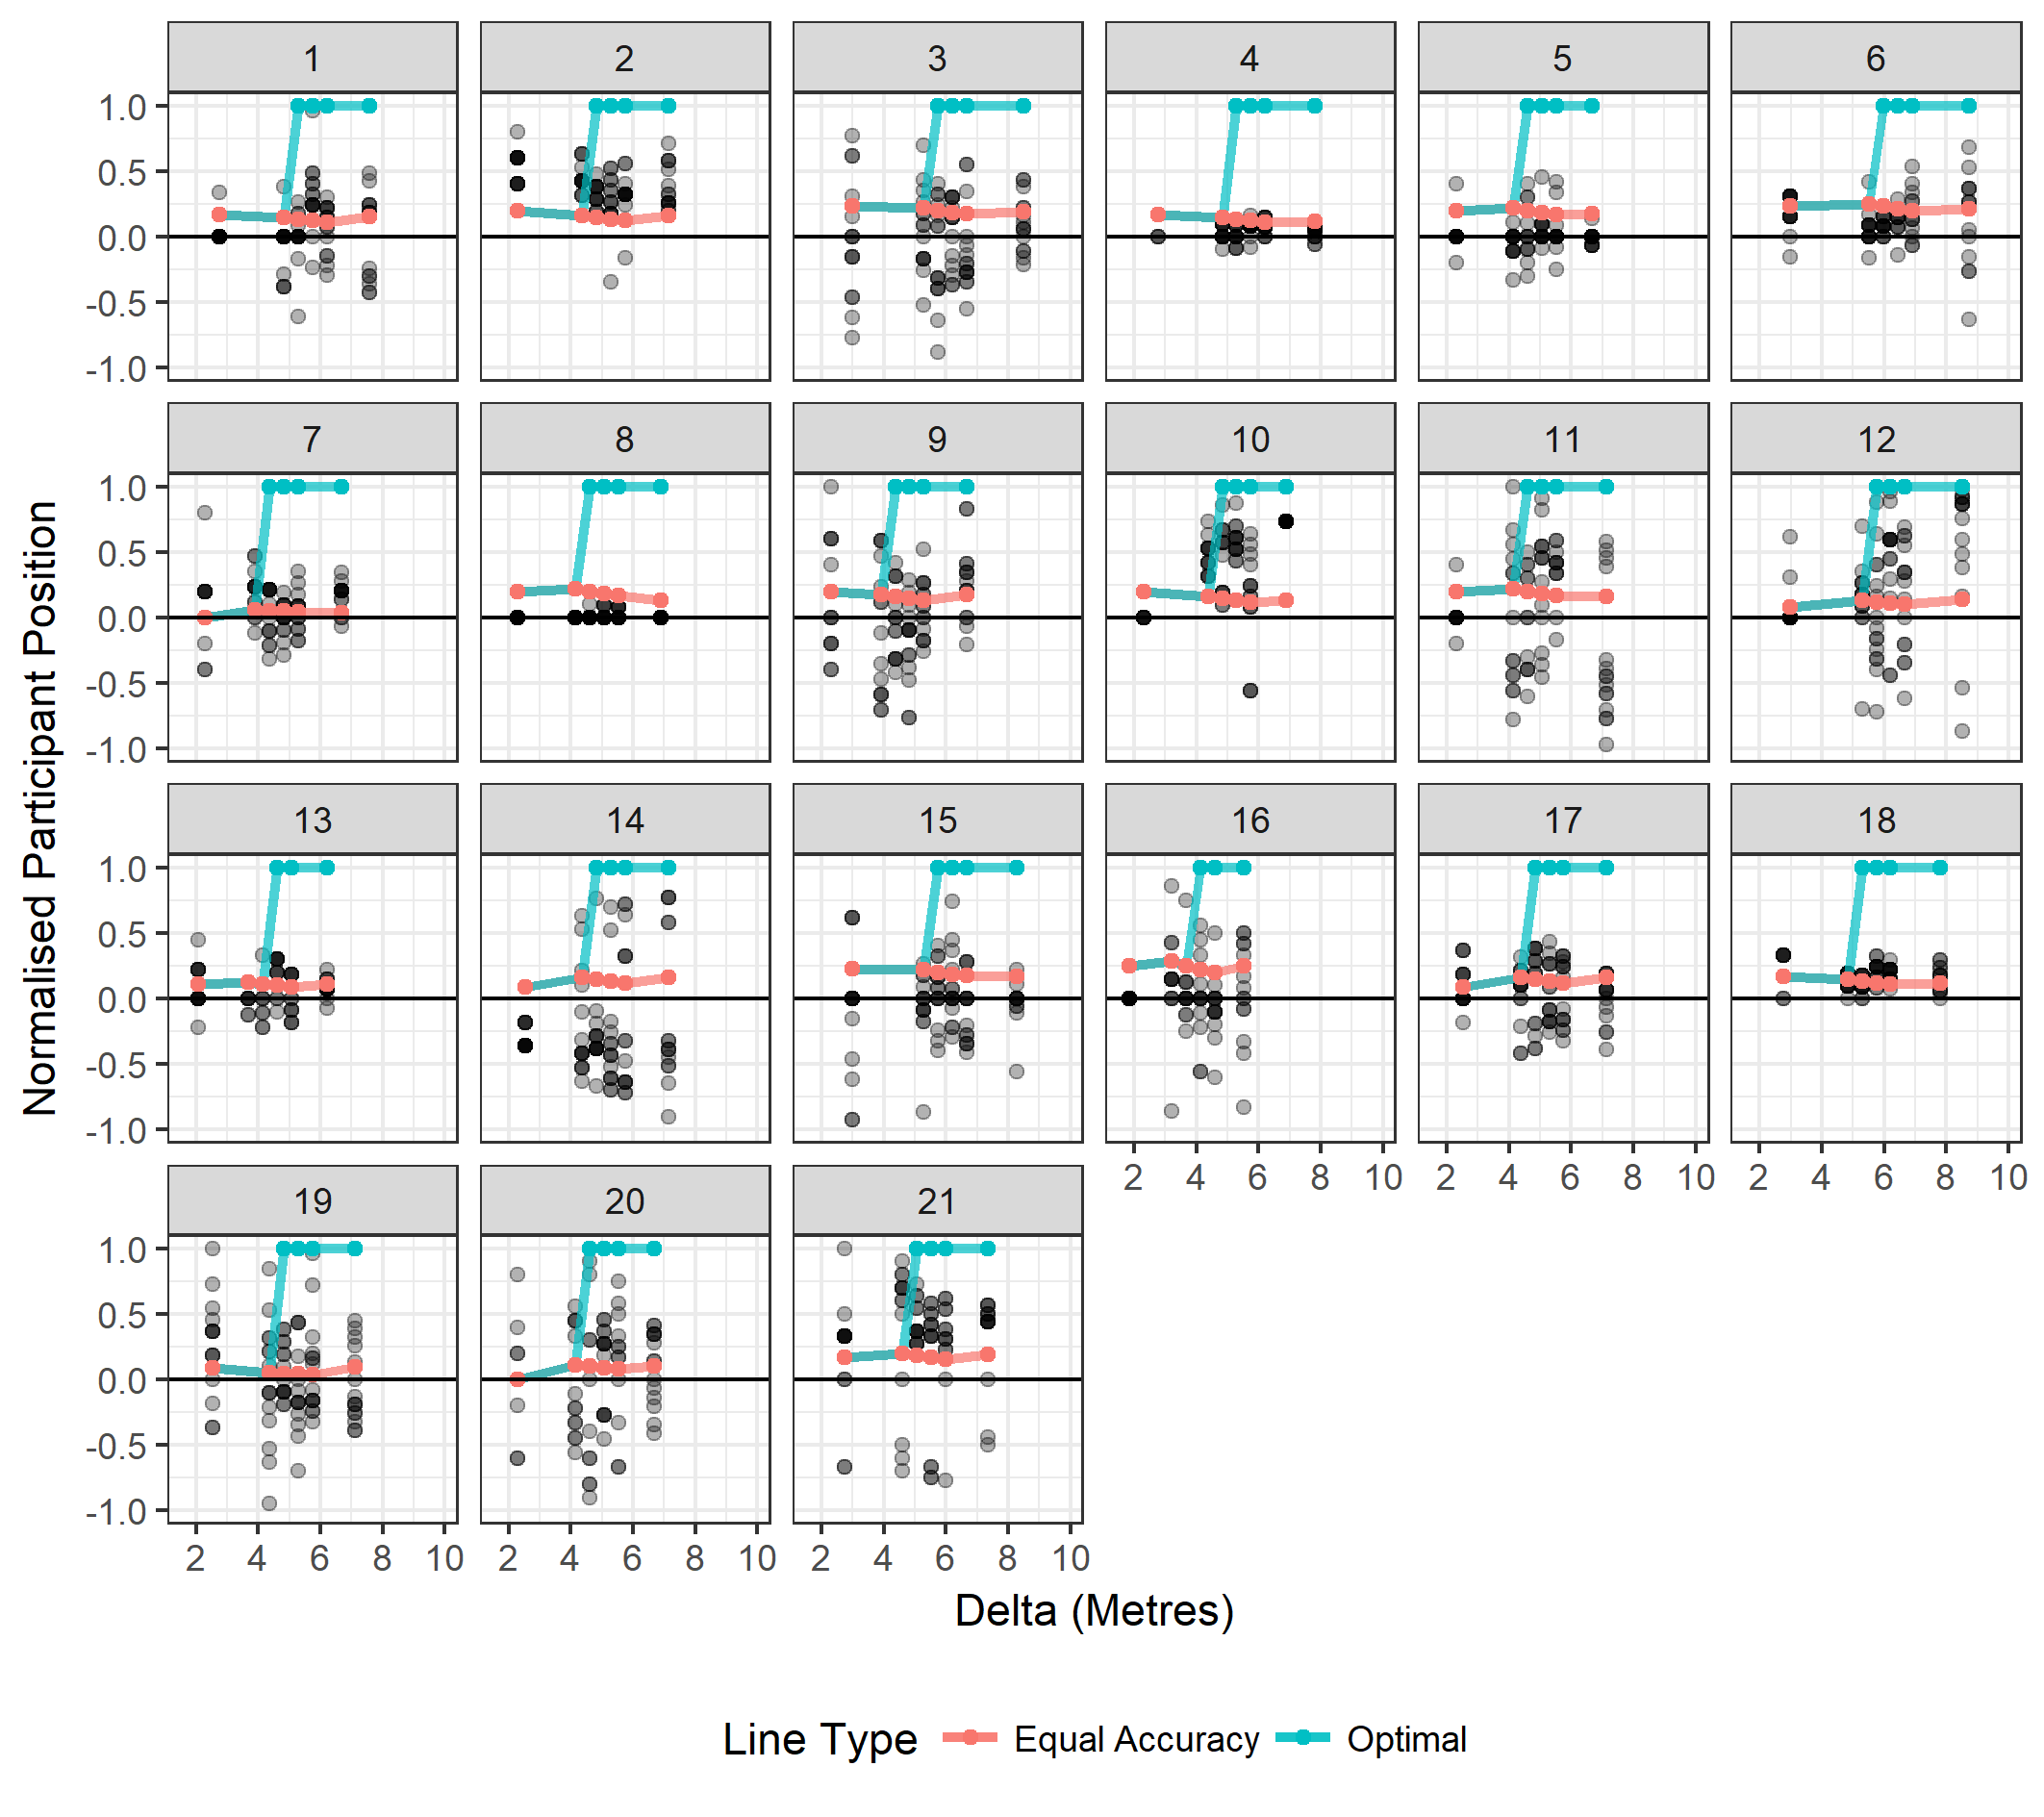
\includegraphics[scale=0.9]{Figures/Experiment_3_Hoop_size/Session_2_plot}
	\centering
	\captionsetup{justification=centering}
	\caption{Standing positions for each participant normalised from 0 to 1. The lines represent the optimal standing position for each separation, and also the position at which accuracy for both hoops is equalised. Darker dots indicate participants stood at this point more often than the lighter shades.}
	\vspace{-0.5cm}
	\label{fig:Session2-HoopSizes}
\end{figure}

\paragraph{} As with previous experiments, participants did not appear to behave in an optimal manner. Participant 10 appears to be the closest to optimal, but falls short as they do not fully commit to standing next to one hoop in the furthest separations. For the most part, it would appear that participants tended to stand slightly closer towards the smaller hoop than the larger hoop (as can be seen in Figure \ref{fig:Session2-HoopSizes}).

\paragraph{} To confirm this, a General Linear Mixed Effects model with a binomial link was used. For the model, the small hoop being on the left or right was used a predictor for wether the participant stood either on the left or right of centre. The results of this model were significant suggesting that pariticipants were more likely to stand towards the small hoop than the large one (the model specification can be seen below). This suggests that participants were somewhat aware that their chances would improve slightly should they have stood slightly closer to the smaller hoop. This is in line with the data presented by \cite{CHAPMAN2010168} in that the participants were positioning themselves in such a way that may have given them a more equal chance of success should either target be the target for that trial.

\begin{figure}[!ht]
	\centering
	\begin{BVerbatim}
	StoodLeftofCentre ~ SmallHoopLeft + (1|participant), family = binomial
	\end{BVerbatim}
\end{figure}

\subsubsection*{Accuracy}
\begin{figure}[ht!]%{L}{0.5\textwidth}
	%\vspace{-0.7cm}
	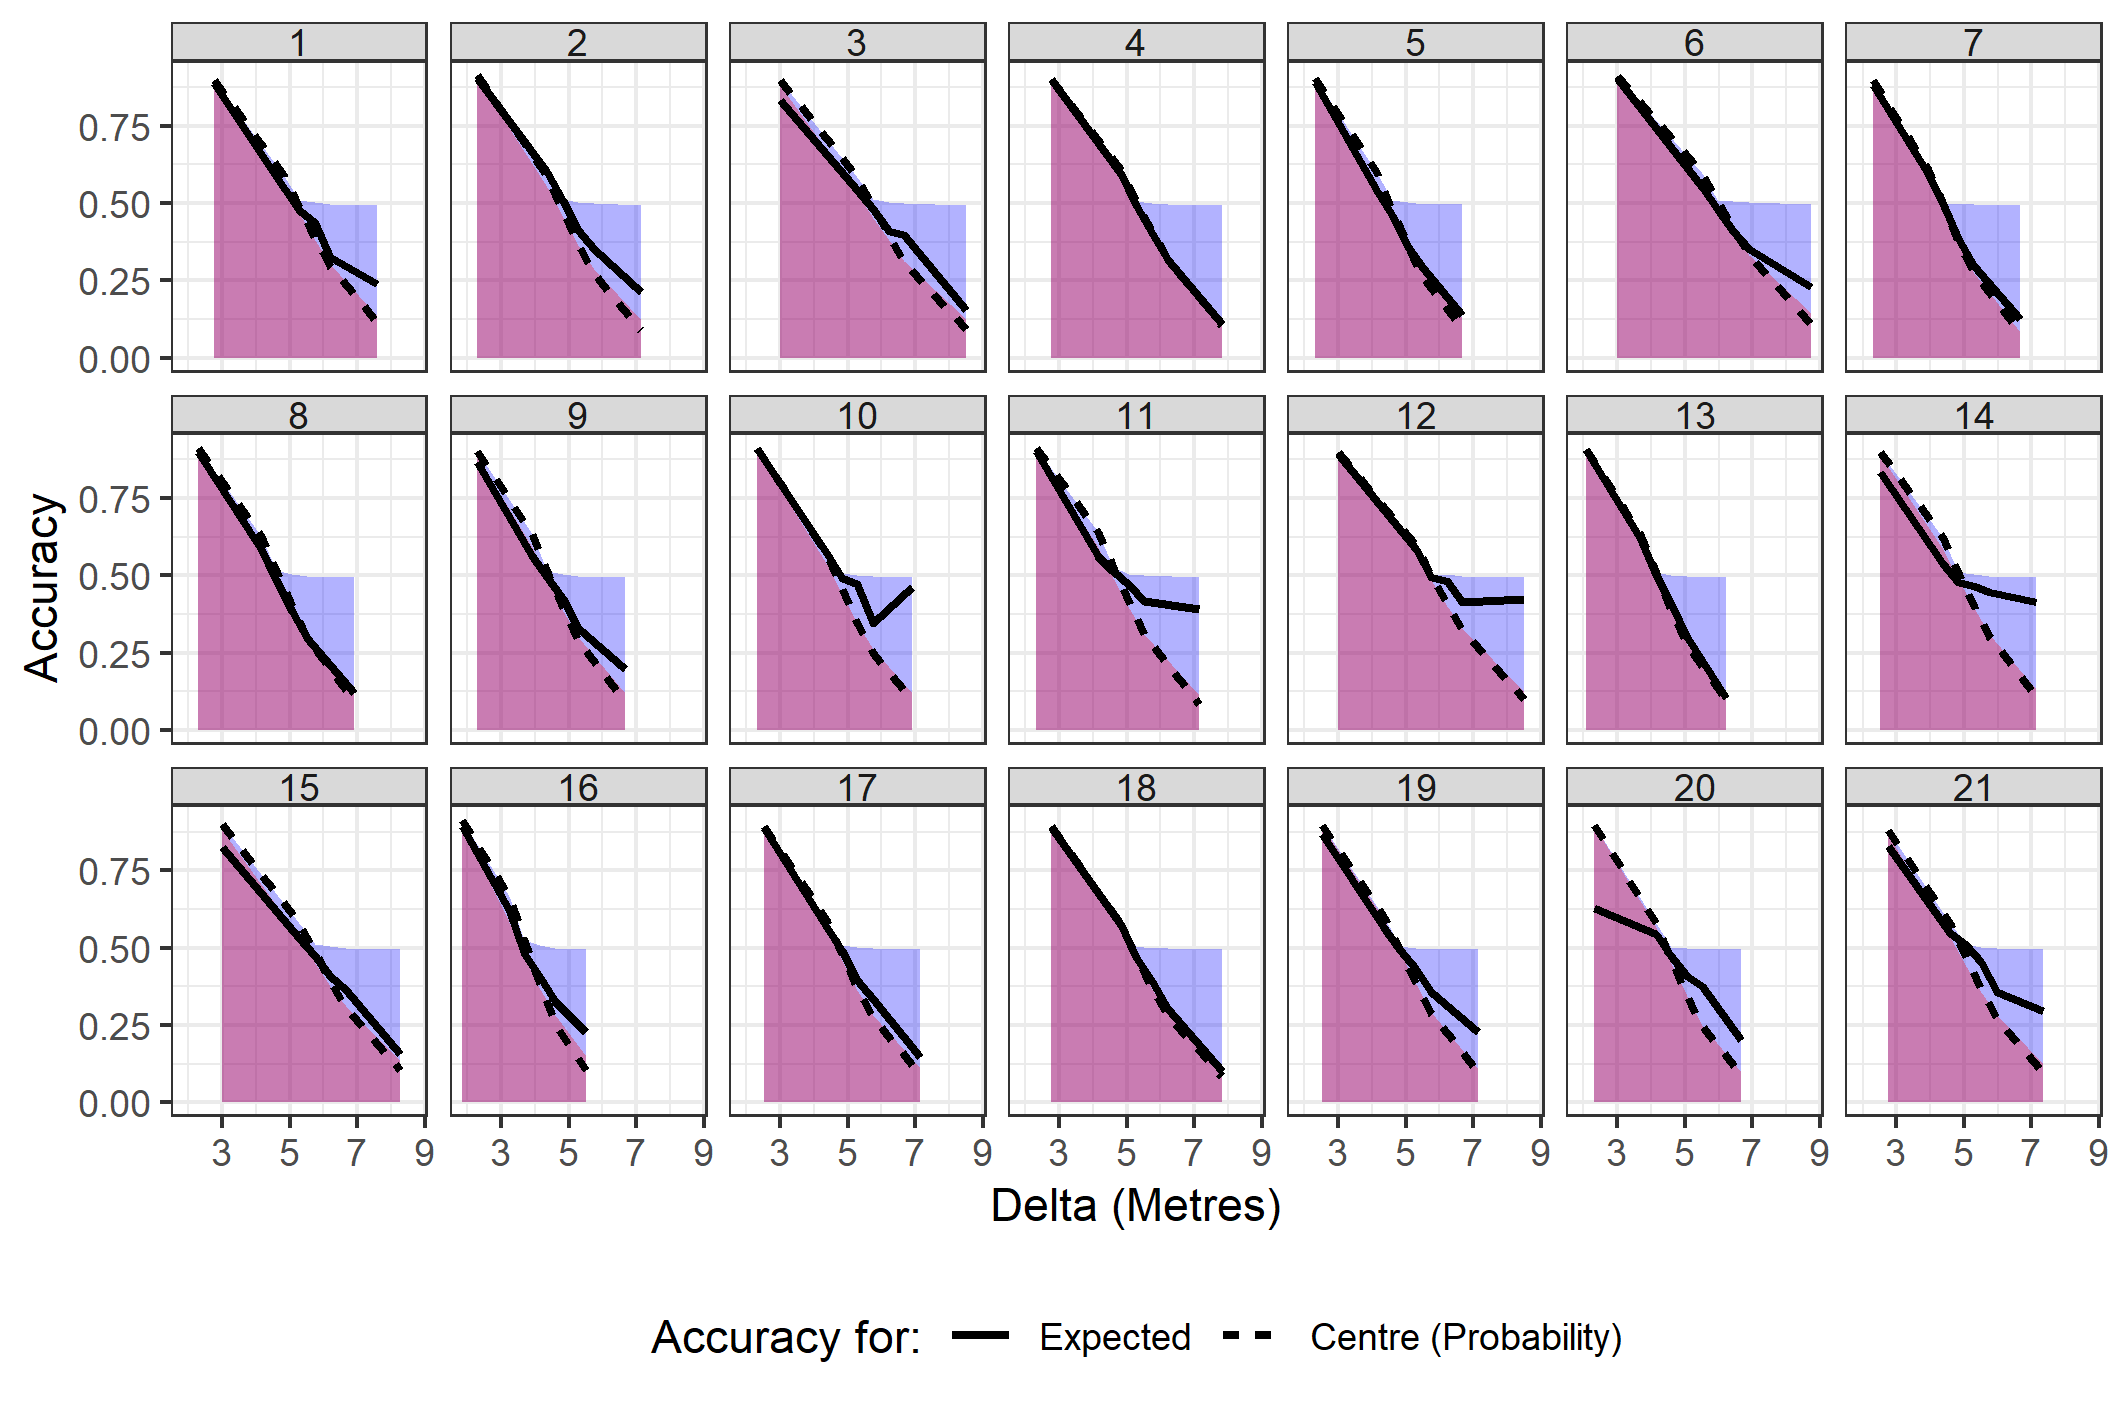
\includegraphics[scale=0.9]{Figures/Experiment_3_Hoop_size/Accuracyshaded_regions}
	\centering
	\captionsetup{justification=centering}
	\caption{The upper limit of the red shaded region shows the accuracy that would have been expected had participants stood equidistant from both hoops. The upper limit of the blue region shows accuracy should the participant have stood in the optimal position. The two lines show expected accuracy had they stood in the centre of probability (dashed line), and expected accuracy given where they actually stood (solid line.)}
	\label{fig:Session2-Hoopsizes-Accuracy}
\end{figure}

\paragraph{} Upon inspecting Figure \ref{fig:Session2-Hoopsizes-Accuracy}, there is little noticeable difference between the expected accuracy should the participant have decided to stand equidistant from each hoop or in the position that offered the participant more equal chance of success. Additionally, by creating a more tangible situation in which there is a clear reason to prioritise one target over the other, participants generally still do not appear to reach the optimal solution. Participants 10, 11, and 12 are close to achieving optimal accuracy for both the closest and furthest hoops, however, as can be seen in Figure \ref{fig:Session2-Hoopsizes-Accuracy}, they still fall short of reaching optimal accuracy. 

\subsection*{Discussion}
\addcontentsline{toc}{subsection}{Discussion}

\paragraph{} In \textit{Experiment 2}, the intention was to provide participants with a more tangible experience of one of the potential targets being more rewarding than the other. Similar to the results of \cite{CHAPMAN2010168} and \cite{Hudson2007probmove}, the participants in this experiment appeared to demonstrate a general tendency to move towards a position that would offer them a more equal chance of success. This is demonstrated by participants on average standing towards the smaller hoops in this task. However, this change to the paradigm still did not facilitate a better understanding of the task that would lead to an optimal strategy being implemented. 


\section*{Experiment 3: Two Throws}
\addcontentsline{toc}{section}{Experiment 3: Two Throws}

\subsection*{Preface}
\addcontentsline{toc}{subsection}{Preface}
\paragraph{} The search for patterns can cause people to perform tasks in a less than optimal way due to this being a cognitively demanding task in itself \citep{wolford2004searching}. In \textit{Experiments 1 \& 2}, there was still the possibility for participants to search for patterns to exploit which may have interrupted the use more relevant information. As such, in \textit{Experiment 3} the aim to was to remove this from the task design and thus remove any reason for participants to try and "discover" an underlying pattern in the task. To do this, instead of telling participants that one of the potential locations would become the target, they were instead to try and achieve both on every trial. 

%\paragraph{} Lastly, the two previous experiments still have the potential for participants to be distracted by the search for a pattern. \textit{Experiment 3} removed any potential for a pattern by offering participants the chance to attempt both goals regardless of what decision they made. The logic for performing optimally was still the same, as focussing exclusively on one potential target when the task was hard would still produce the greatest rate of success. The only difference here is that there is no potential for participants to be trying to figure out which target would be the actual target for that trial.  

\subsection*{Methods}
\addcontentsline{toc}{subsection}{Methods}
\subsubsection*{Participants}
\paragraph{} In total, 18 participants (8 male) took part in this experiment, with an average age of 22.1 (\textit{SD} = 3.02). Participants were recruited via word of mouth.

\subsubsection*{Procedure}
\paragraph{} This experiment followed the same protocol as in Experiment 2. The main differences were that for both sessions, the hoops were all the same size, and in Session 2 participants were given two bean bags to throw. There was only one hoop size used in experiment which measured $0.4cm$ in diameter.

\paragraph{} Session 1 followed the same structure as in Experiment 2, however, now there was no need to test the participants with different hoop sizes. Session 2 was split into two conditions; the \textit{One-Throw} and the \textit{Two-Throw} condition. The order of these was counterbalanced across participants. The stated goal for both conditions was to get as many bean bags into the hoops placed before them.

%put how it's the same here
\paragraph{} Session 2 was divided into two conditions with each participant experiencing both. The first condition was the \textit{One-Throw} which followed the same paradigm as in \textit{Experiment 2}, however, each hoop was the same size and so standing equidistant from both would give participants an equal chance at each target. The distances were calculated in the same way as in \textit{Experiment 2}, but again only one hoop size was used. 

\paragraph{} The \textit{Two-Throw} condition differed with respect to the \textit{One-Throw} in that participants would be throwing towards both hoops on each trial. They were still instructed that the goal was to get as many bean bags into as many hoops as possible. Participants would still select one bean bag from a bag containing nine with three of each colour. They were then handed a second bean bag of the same colour from a separate pile. Participants were still instructed to choose somewhere to stand, at which point they would notify the experimenter and they would throw the bean bags to each hoop in whichever order they preferred. 

\subsection*{Results}
\addcontentsline{toc}{subsection}{Results}
\subsubsection*{Standing Position}
\begin{figure}[ht!]
	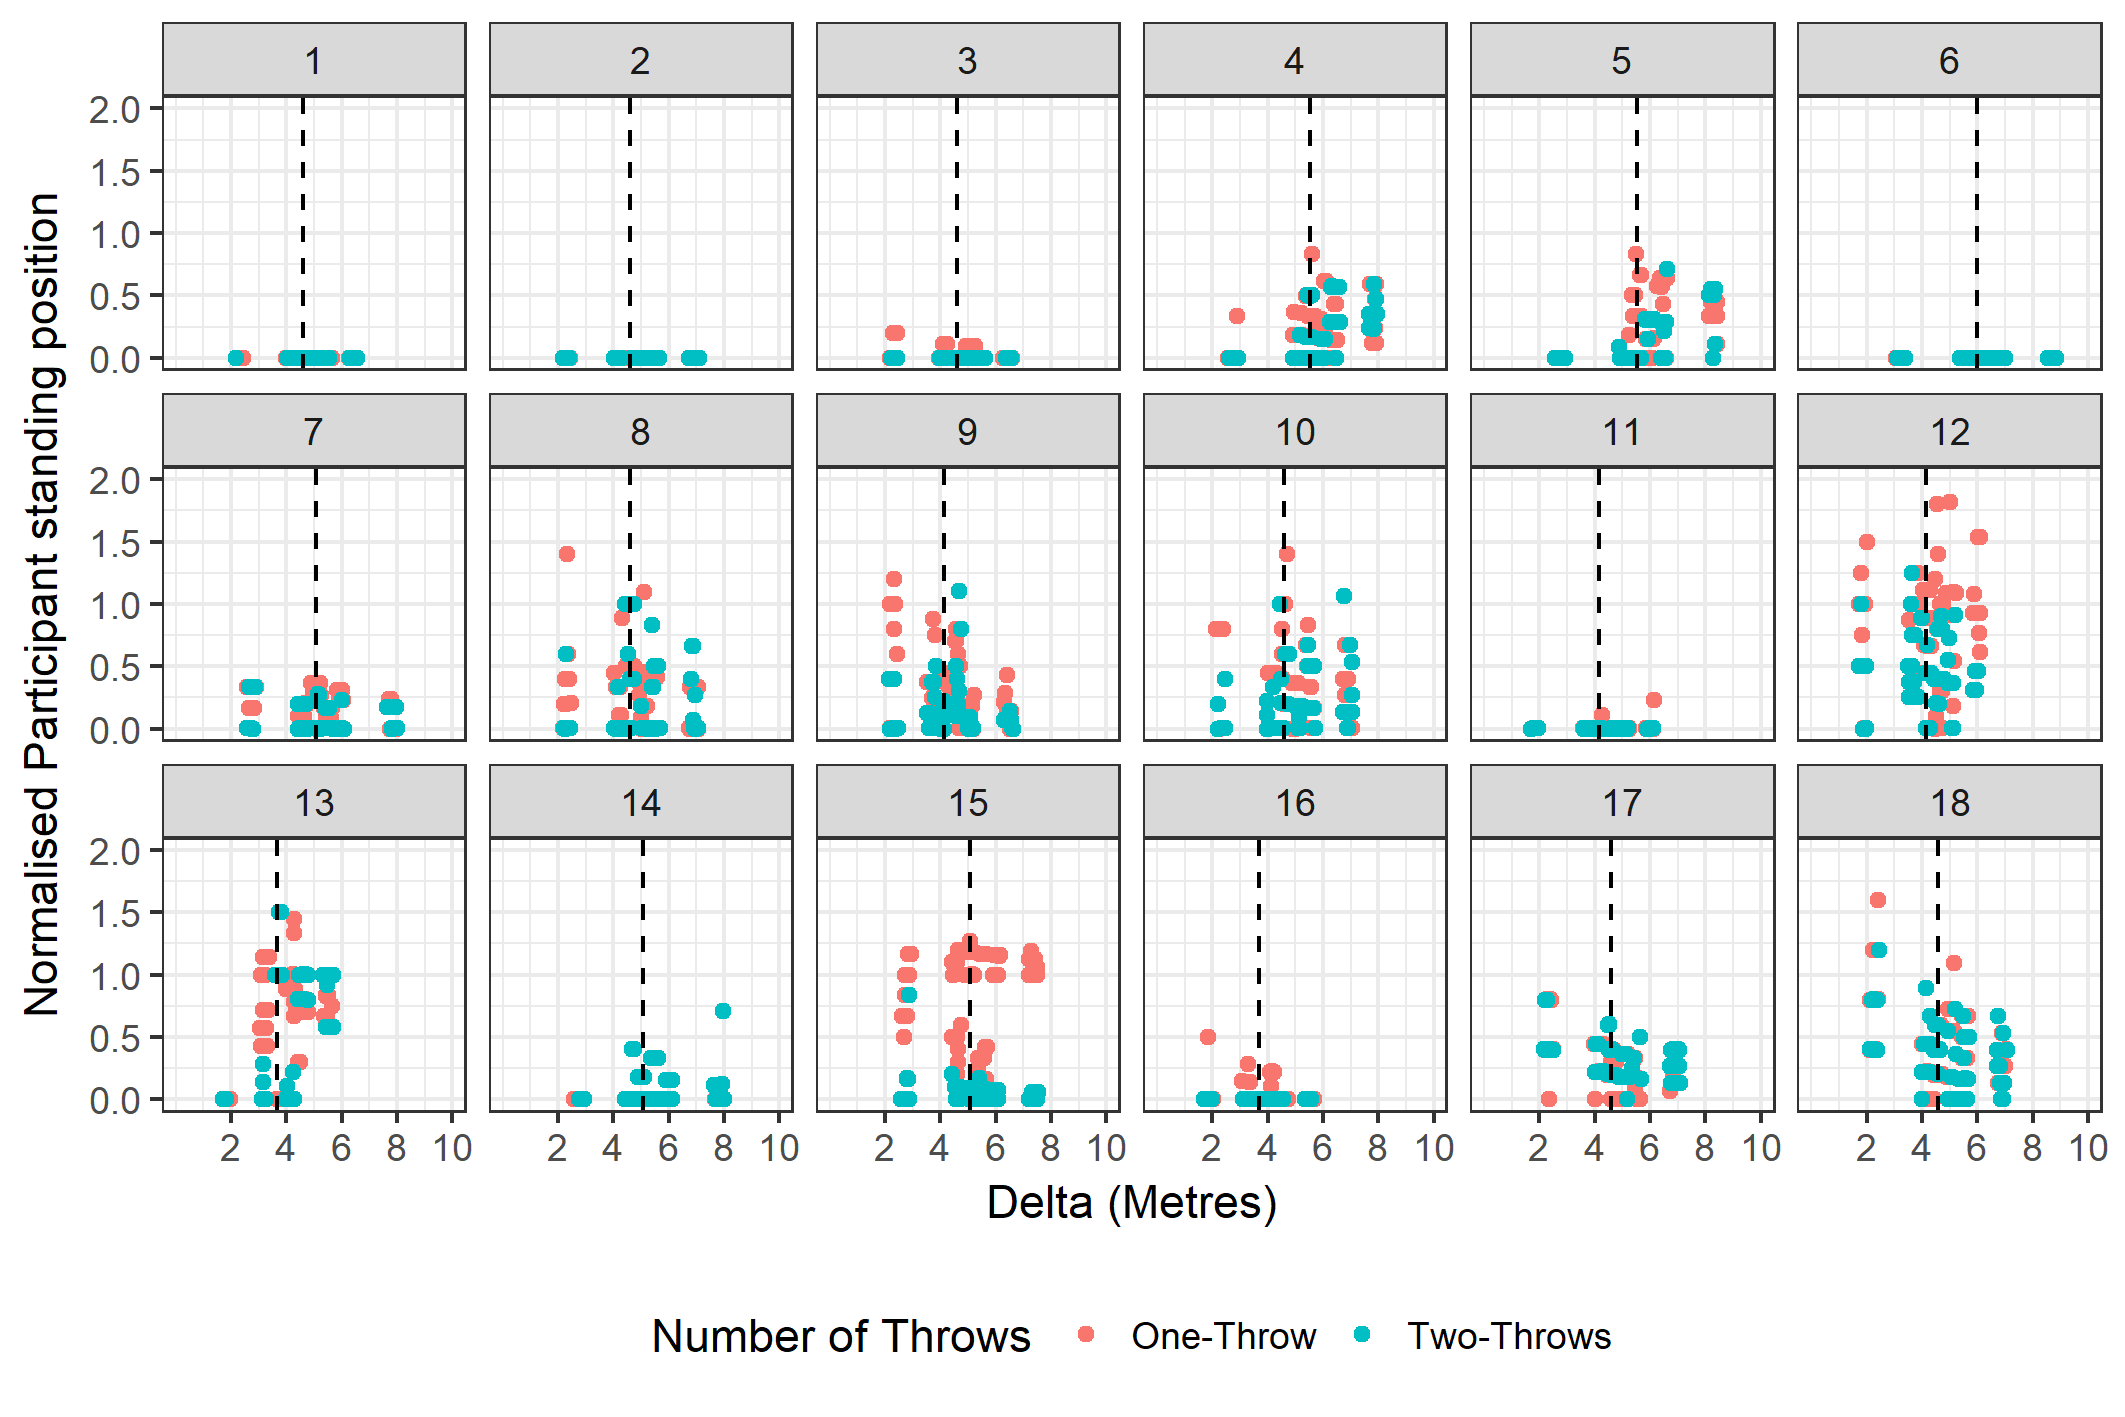
\includegraphics[scale=0.9]{Figures/Experiment_2_Two_throw/Part2_BOTH_AvG_allpoints}
	\centering
	\captionsetup{justification=centering}
	\caption{Standing positions from Session 2 for each hoop separation and number of throws. The $y$ axis is normalise so 0 means the participant stood at the centre, while 1 means they stood next to one of the hoops. Each point is where the participant stood for each trial, for each separation \textit{Delta}, and No. of throws. The vertical black line represents the point at which the participant should have switched from standing equidistant from both hoops (i.e 0) to standing next to one of the potential target hoops (i.e. 1).}
	%\vspace{-20pt} 
	\label{fig:Session2-TwoThrows} 
\end{figure}

\paragraph{} From visually inspecting Figure \ref{fig:Session2-TwoThrows}, one can see that for the most part, the number of throws had no real effect on where particpants chose to stand. The only participant that appears to show some difference is participant 15 and this is in the oppossite direction to what would have been expected should removing any reason to search for patterns had impeded participants' ability to figure out the optimal strategy. 

\subsubsection*{Accuracy}

%Could make this plot wider or figure out how to make it wrap nicely?
\begin{figure}[ht!]%{L}{0.5\textwidth}
	%\vspace{-0.7cm}
	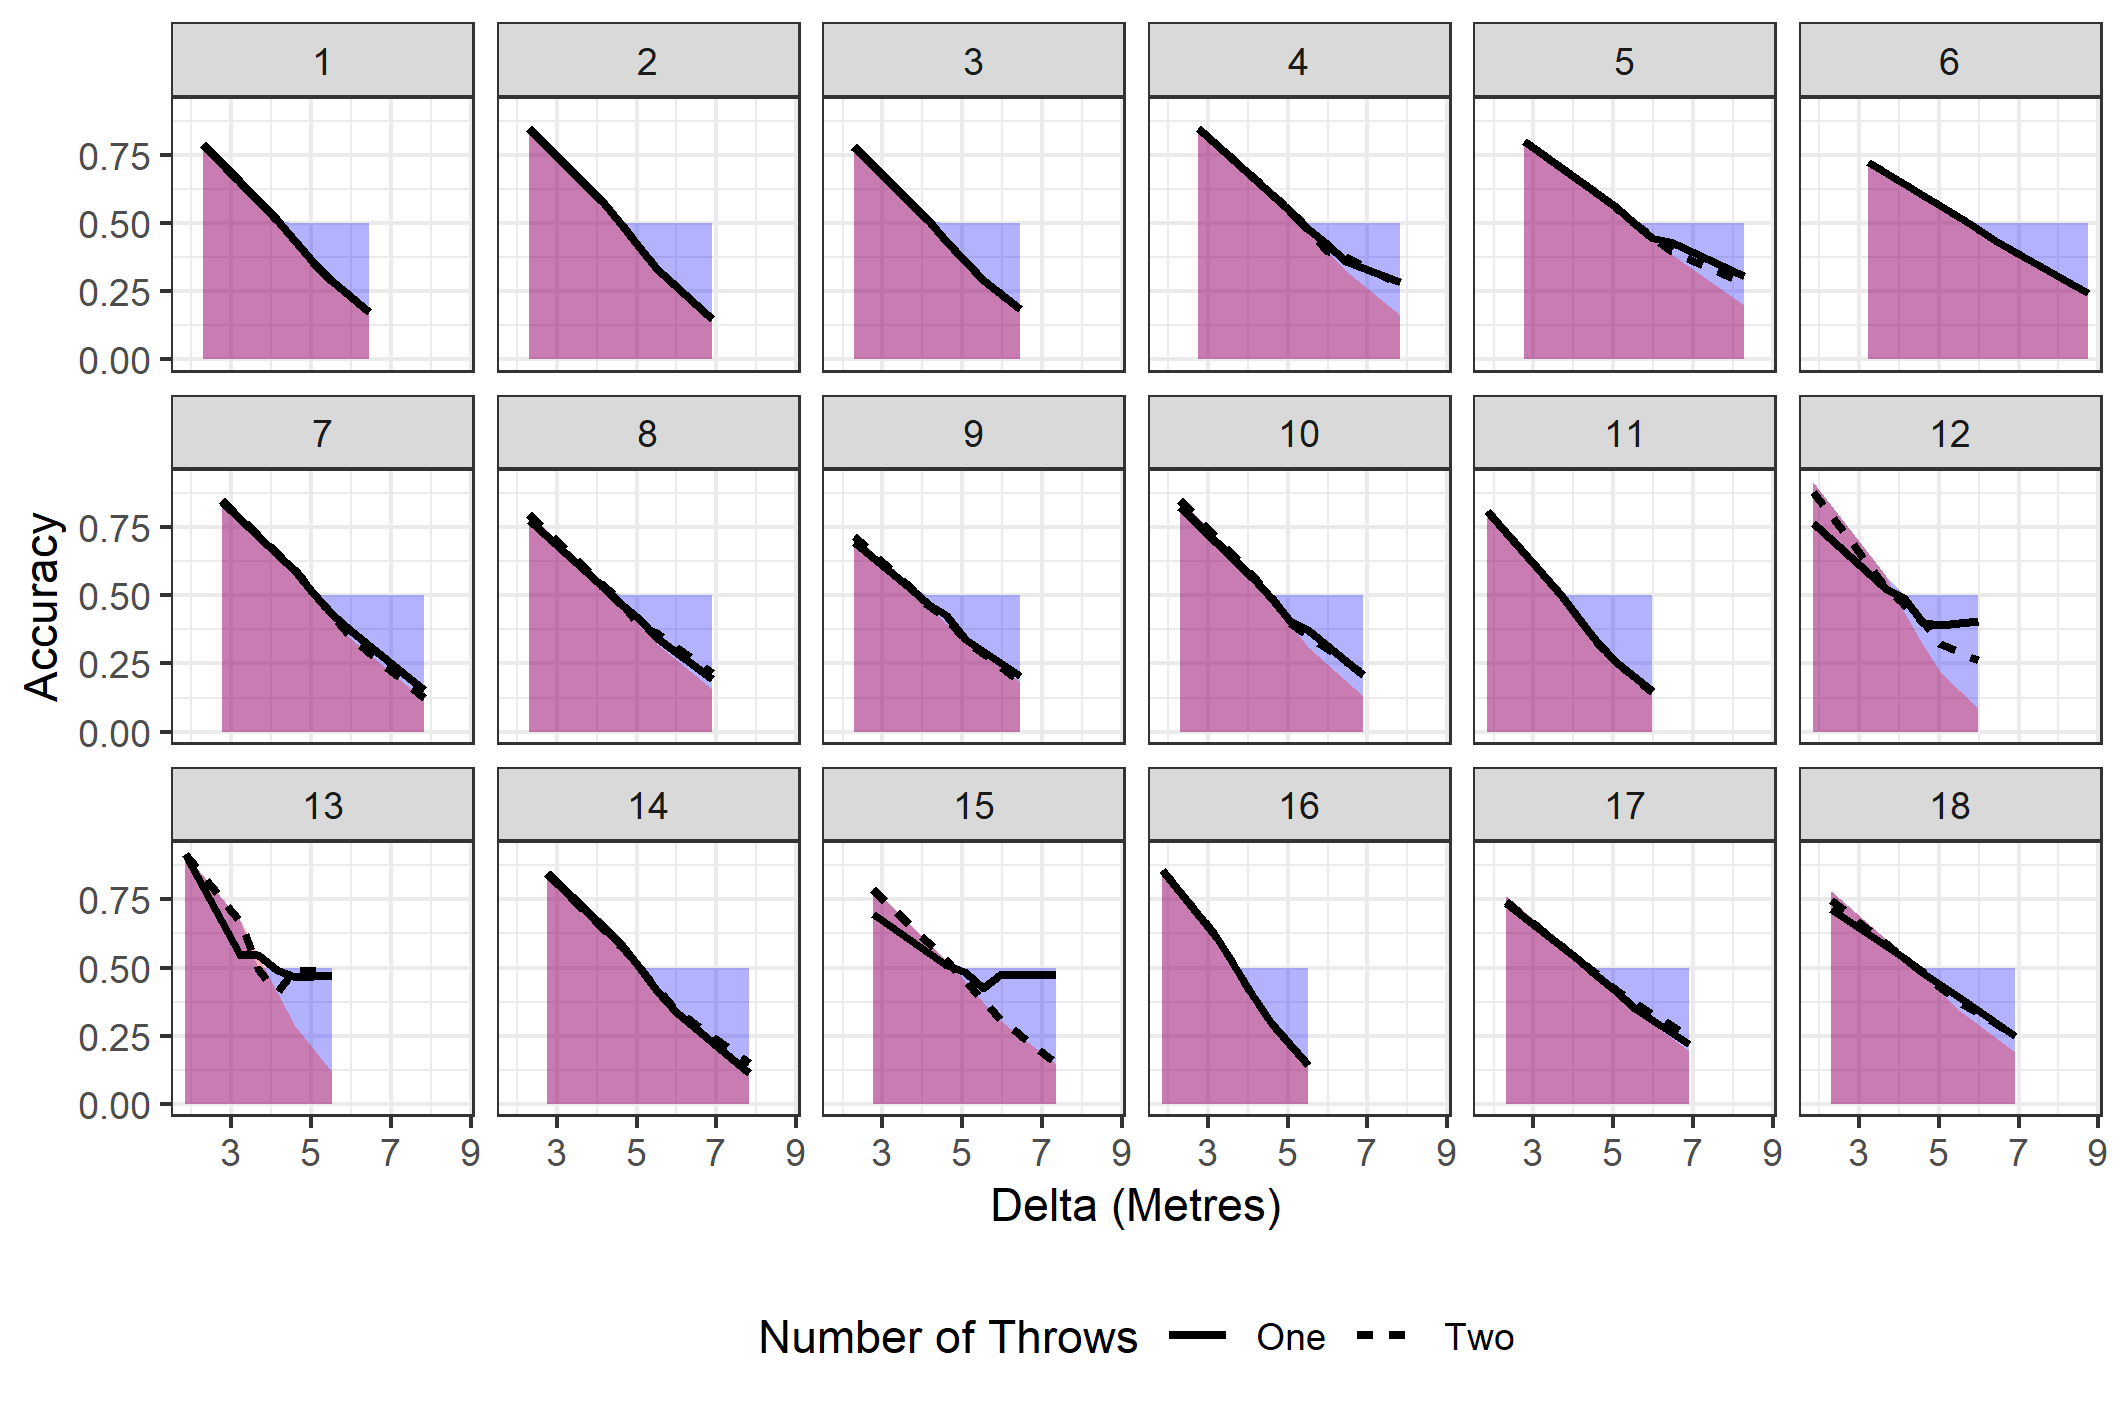
\includegraphics[scale=0.9]{Figures/Experiment_2_Two_throw/Accuracyshaded_regions}
	\centering
	\captionsetup{justification=centering}
	\caption{These plots show participants expected accuracy given their standing positions as the two black lines. The upper limit of the region shaded red is what would be expected if they had stood in the centre for every trial. The upper limit of the region shaded blue is the expected accuracy had the participants employed the optimal strategy.}
	\label{fig:Session2-TwoThrows-Accuracy}
\end{figure}

\paragraph{} Inspecting Figure \ref{fig:Session2-TwoThrows-Accuracy} demonstrates that most participants achieved an accuracy that would be expected had they followed the Centre strategy. The one exception to this is participant 13 who appears to achieve an accuracy close to the optimal strategy. By looking at the participant's standing positions in \ref{fig:Session2-TwoThrows}, this would make sense as they appear to switch at an appropriate point given their own ability to perform in this task. Although they did appear to stand outside the range for some distances, it appears that they were were more likely to stand in a central position for the smallest distances, and towards one of the sides for the larger distances. 

\subsection*{Discussion}
\addcontentsline{toc}{subsection}{Discussion}
\paragraph{} Much like in the previous experiments, most participants still failed to perform optimally in the task even when any reason to search for patterns was removed. Again, there was one participant (participant 13) that appeared to perform the task in a somewhat optimal manner and achieved a reasonably high level of accuracy. From these results, it would appear that the search for patterns is not as distracting as one might expect, as even after having removed any possibility for a pattern to exist, participants still fail to fully commit to focussing their resources on one target.


\section*{Experiment 4: Unequal Reward}
\addcontentsline{toc}{section}{Experiment 3: Unequal Reward}

\subsection*{Preface}
\addcontentsline{toc}{subsection}{Preface}
\paragraph{} As mentioned before, in \textit{Experiment 1}, participants were tasked with tracking a fairly abstract concept of probability. They would have needed to recognise that the location with the highest likelihood of containing the target would reward them with the greatest rate of return in the long term should they have consistently selected this option. As such, it is possible that participants did not see the more likely option as being more valuable, but instead would try to make use of this information in another way. As mentioned in the introduction, \cite{Goodnow1955} demonstrated that when participants were offered a financial incentive for success, they were more likely to make use of a maximising strategy over the, in this context, less optimal alternative of probability matching. In \textit{Experiment 4}, we attempted to investigate this by intorducing a very clear, external reward for successful performance in the task. 

\pararaph{} However, as discussed above in relation to the similarity of results obtained by both \cite{clarke2015failure}, who did not pay participants, and \cite{morvan2012human}, who did pay participants, both targets were not necessarilly equal in value for this experiment. In this task, participants were given 50p on each trial and were told they could choose to split the money equally across the potential targets (i.e. 25p/25p) or unequally (i.e. 40p/10p) prior to each trial. Using this setup, we are able to investigate whether participants that are more likely to opt for the unequal split would demonstrate a stronger tendency to stand closer to one hoop over the other.  

\subsection*{Methods}
\addcontentsline{toc}{subsection}{Methods}
\subsubsection*{Participants}
\paragraph{} \textit{Fill this in when we get the results}

\subsubsection*{Procedure} 
\paragraph{} Participants signed a consent which contained details about the reward schedule and how much they could expect to achieve on average. All participants were given £4 as a baseline and were told that they could expect to earn an addtional amount ranging from £0 to £4.80 depending on their performance. They were also told that we expected them to earn between £1.50 and £2.50 on average.  

\paragraph{} This experiment made use of the \textit{Throwing Task} and as such, followed a similar procedure to that of \textit{Experiments 2 \& 3}. However, in this experiment, both the measuring and decision phases took place in one session. First, participants were taken to the paved area in order to measure their throwing ability across several distances. After which, they were taken to perform a computer task which was simply to occupy their time whilst the experimenter set up the hoops for the second session much in the same way as before. For this computer task, participants were to detect the presence or absence of a target polygon that was presented amongst a mixture of polygons for 200ms. For the final task, participants were taken back to the paved area to perform the decision phase. 

\paragraph{} There were two main changes to the paradigm for this experiment. Firstly, instead of calculation 3 points, 4 were calculated so as to avoid using the somewhat ambiguous 50\% accuracy point. Now, the points at which participants were 90\%, 75\%, 25\%, and 10\% accurate were used. Addtionally, participants were now told they had 50p to split between the two target items in one of two ways. They could either split it equally across both potential targets (25p/25p) or make it an 80/20 split (40p/10p). Participants were asked how they would like to split the money before they made a choice about where to stand. If they opted to make an unequal split, they were asked which hoop they would like to be worth 40p and which 10p. Participants were informed that the target hoop had been predetermined so that each hoop was equally likely to be the target on each trial and that there was no pattern. It was reaffirmed that any money they earned by successfully throwing the bean bag into the target hoop would be given to them upon completing the experiment. Participants would then pick a place to stand, at which point they would be told which hoop was the target for that trial and their standing position was recorded covertly. 


\subsection*{Results}
\addcontentsline{toc}{subsection}{Results}

\begin{figure}[ht!]%{L}{0.5\textwidth}
	%\vspace{-0.7cm}
	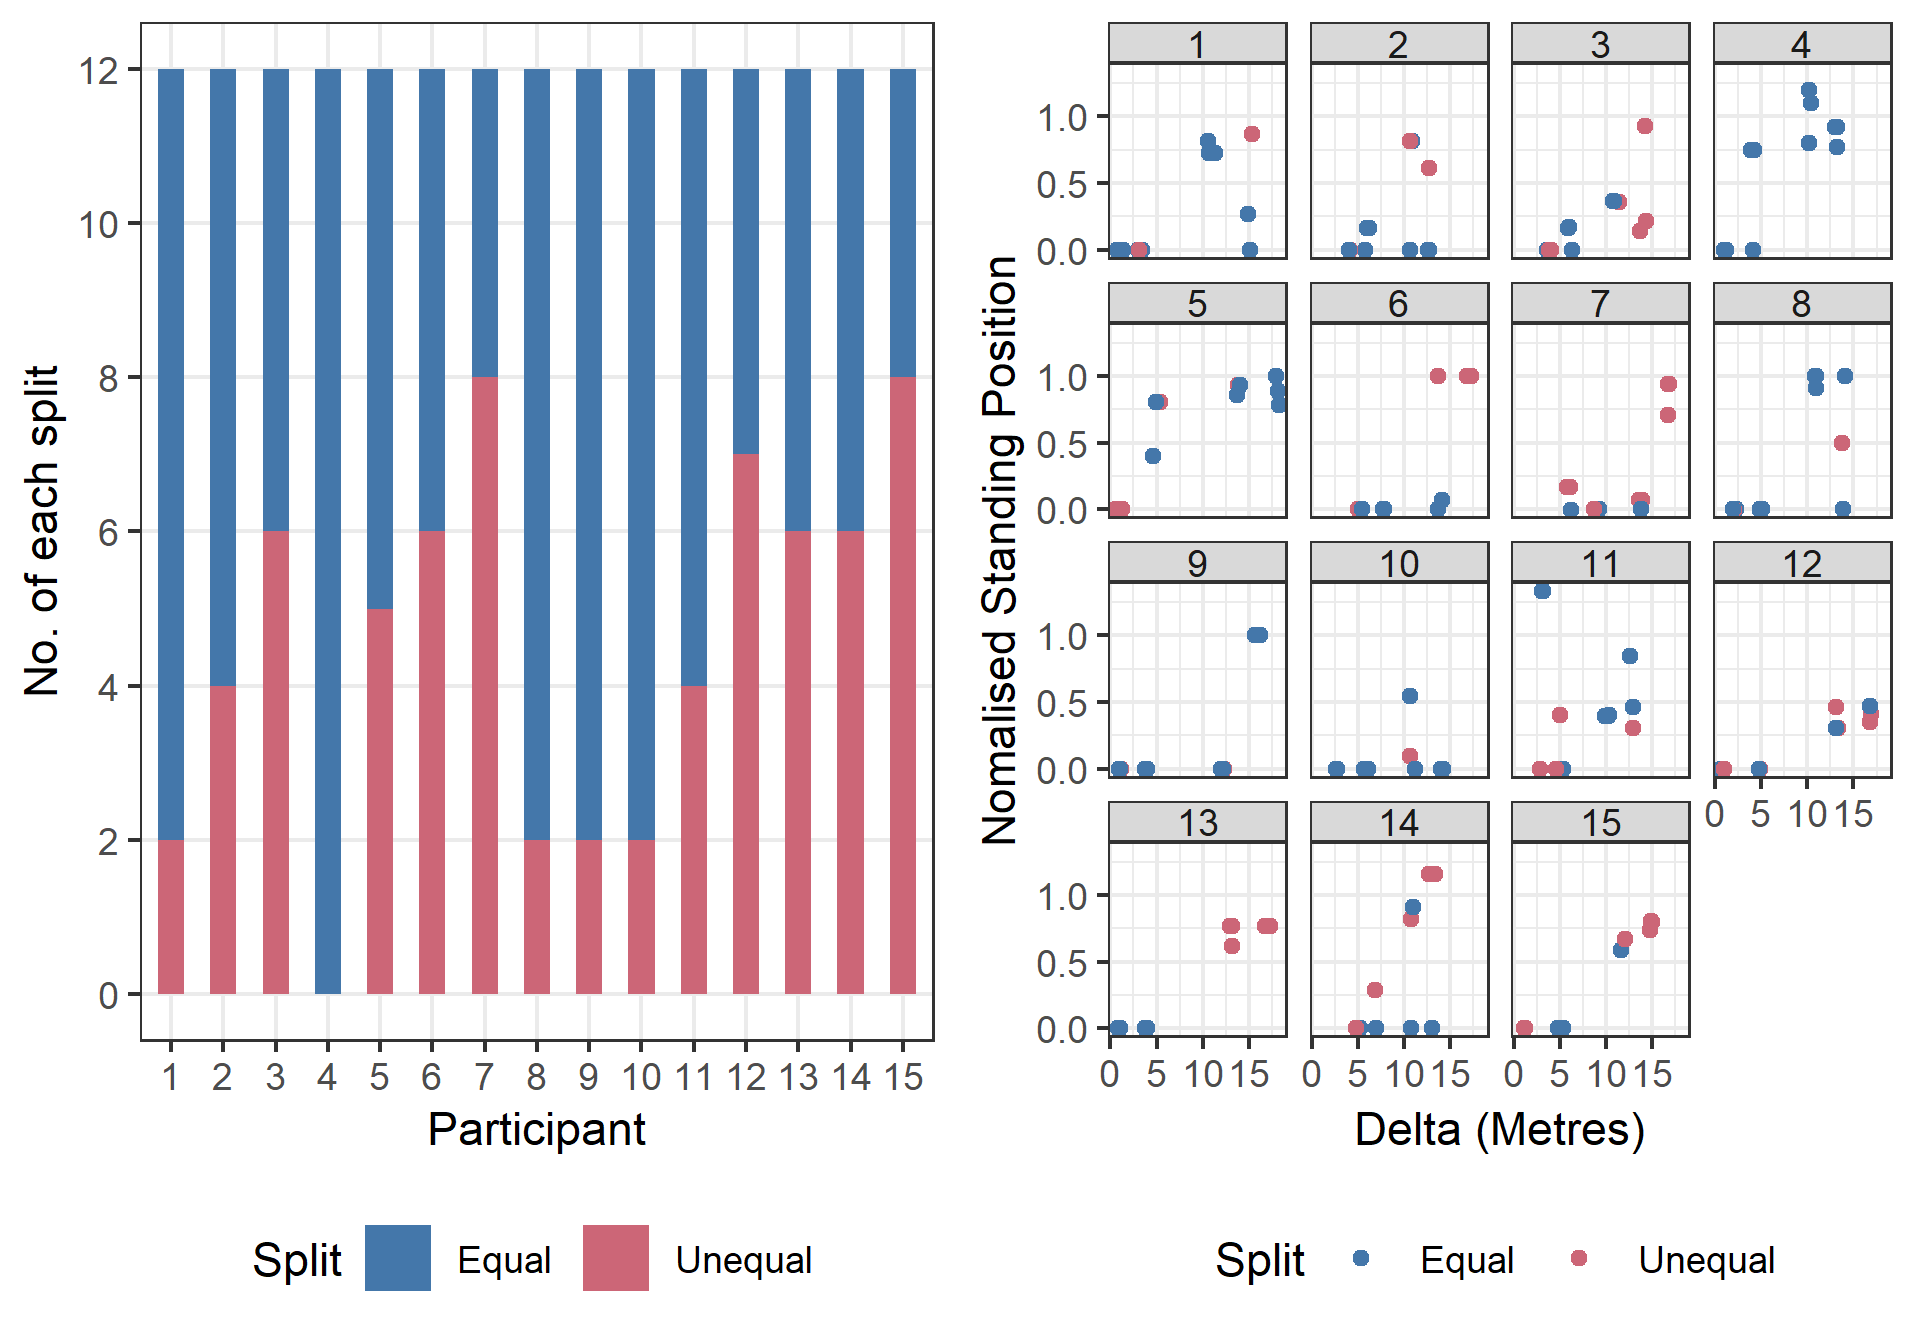
\includegraphics[scale=0.9]{Figures/Experiment_5_Unequal_Reward/prop_and_position}
	\centering
	\captionsetup{justification=centering}
	\caption{These plots show the proportion of times each participant opted for an unequal or equal split (\textit{left}) and their normalised standing position during the decision phase colour coded to show whether the trial was an unequal or equal split (\textit{right})}
	\label{fig:DecisionPhase_Reward}
\end{figure}

\subsection*{Discussion}
\addcontentsline{toc}{subsection}{Discussion}

%if an image is causing problems with text not detecting a new page, use this to sort that out
%\clearpage
%\newpage

\section*{General Discussion}
\addcontentsline{toc}{section}{General Discussion}
\paragraph{} The results from each of the experiments in this paper follow the same trend as observed in \cite{clarke2015failure} and \cite{James2017}; the majority of participants fail to perform the task using the optimal strategy. \textit{Experiments 1 \& 2} attempted to make one option more attractive in the sense that it would either contain the reward more often, or be slightly easier to achieve. This was done so as to remove the need to make an arbitrary decision once the task became more difficult. The results of these two experiments appear to rule out the idea that participants were unable to make use of the optimal strategy due to difficulty encountered when trying to decide which side to choose. 

\paragraph{} However, these two experiments do offer some insight into information people may be attempting to make use of when performing these sorts of tasks. For example, in \textit{Experiment 1}, participants generally were more likely to prioritise one side over the other when there was a reason to do so. Although they did not quite make use of this information in an optimal way (i.e. by exlcusively fixating the more likely box) as would be expected \citep{koehler2014probability}, there was a difference when compared to a situation in which each option was equally likely. This adds further support to the notion that people are sensitive to this information and will make use of it when making decisions \citep{wolford2004searching,yellott1969probability}. Due to this, it is possible that participants were in fact making an attempt to maximise their rate of success, but were doing so using a suboptimal strategy \citep{Gao2015}.  

\paragraph{} In \textit{Experiment 2}, participants generally stood close to the smaller hoop which demonstrated they had some awareness of their ability. This was much the same in \textit{Experiment 3}; even though participants would have achieved an accuracy level of at least 50\% for each trial had theystood next to one hoop, they still failed to commit to one side. Both these results suggest that participants were trying to maintain a relatively equal chance of success. This failure to fully commit to one option has been demonstrated in other tasks such as those employed by \cite{CHAPMAN2010168} and \cite{Hudson2007probmove}. It may be that this failure to fully commit to focussing exclusively on achieving one goal shares a similar fundamental misunderstanding with the behaviour of probability matching. In both cases, there would appear to be a reluctance to forgo the reward should it be target that was not selected to be the focus on a particular trial. However, what remains unclear here is whether this is the actual case, or whether participants simply do not recognise a strategy of focussing on one goal as being the better option \citep{kahneman1982judgement}. It's possible that participants do believe that by maintaining an equal chance of success, that they are actually making the choice that gives them the best chance of success. However, this would need to be investigated by asking participants about strategy use. In \cite{Koehler2010}, after having performed as task about predicting the outcome of binary events with one more likely than the other, even participants that engaged in probability matching were more likely to endorse maximising as the better strategy. 

\subsection*{Confidence}
\addcontentsline{toc}{subsection}{Confidence}
\paragraph{} This raises the question of whether participants are making their decisions about where to stand with confidence, or whether they recognise when they are doing something that might not be "correct". \cite{SZOLLOSI20171} presented people with a series of questions with the three items from the Cognitive Reflection Task \citep[CRT: ][]{Frederick2005CRT}. These items are designed so that an inuitive, but incorrect, answer will spring to mind. An example of one of these items the bat and ball problem which goes as follows; \textit{"a bat and a ball cost \pounds1.10. The bat costs \pounds1.00 more than the ball. How much does the ball cost?"} The correct answer is 5p (the bat being worth \pounds1.05), yet many people often state the ball is worth 10p causing the total to be \pounds1.20 \citep{Frederick2005CRT}. In the study by \cite{SZOLLOSI20171}, they gave people many problems like these and also asked participants to give a rating of how confident they were that they had given the correct answer. When tasked with answering the items from the CRT and giving the wrong answer, particiapnts tended to be less confident that they had given the right answer. Additionally, their participants indicated that they had also spent less time trying to figure out the answer to questions they were less confident in. They argued that these coupled together suggest that people recognised that the task was "too difficult" and offered the solution that first came to mind. 

\paragraph{} The idea that people may simply give up and offer the first solution that comes to mind is similar to the idea of "satisficing" \citep{simon1990invariants}. This is when someone finds a task too difficult and as such attempts to solve the problem using little effort such as using a strategy that has worked before in other contexts. It's possible that once participants find the tasks in this paper to be too difficult, they gave up and continued to behave in the same way as before. One way to investigate this would be to use a similar paradigm to that employed by \cite{Kiani759}. In their study, they presented monkeys with a large number of moving dots on a screen and they were to report the "global direction" of the dots (i.e. were they mainly moving to the left or the right). For each correct answer, they receieved an amount of juice In some cases this would be easy to estimate as a large proportion of the dots would be moving as a group. However, in some cases, only a small proportion would be moving in one direction with the rest moving at random. In these situations it became more difficult for them to discern the "global direction" of the dots. On random trials they were offered a third option that would offer a certain reward, but this was worth less than if they gave the correct answer. What they found was that the monkeys would use this option when the task was more difficult. 

\paragraph{} This idea of confidence could easily be incorporated into the tasks used in this paper in order to investigate whether people may simply be satisfising rather than trying to figure out a solution. Much like in \cite{Kiani759}, a third option could be introduced on random trials that would give a small but certain reward. If participants are able to recognise their own ability to perform but cannot figure out the solution to the task, then what would seen is that participants would continue to stand more towards the centre, but only opt for the 3rd, lesser value but certain option, when the task became harder. This would enatil that participants would need to have some sort of performance related reward, and although this does not seem to make a difference when comparing the performance of participants with reward \citep{morvan2012human} and without \citep{clarke2015failure}, it does allow for the hypothesis that participants are simply satisfying to be investigated. %Satisfising is argued to be due to people reaching a certain success threshold and the ceasing to search for alternative strategies that may improve their performance. As such, it would be possible to alter the amount of reward participants would receive if they selected the 3rd option. With a setup like this, it would be possible to investigate whether a lack of confidence in one's capacity to solve this problem results in settling for a relatively low success rate. 

%This paragraph is weak... maybe rephrase it a bit or develop the idea a bit more?
\paragraph{} Additionally, adding a financial incentive for success allows for other potential factors to be investigated. Although in \cite{James2017}, participants were able to give accuracte measures of their own ability, this does not necessarily mean that they would incorporate this information into their decision making. \cite{Goodnow1955} argued that in the context of problem solving, people are more likely to probability match, within a gambling context, people tend to maximise. Within the context of this study, the paradigm could be altered so that participants would have sum of money they would split between each target. For example, they could split the amount equally between each target. If the they were then successful for the selected target, they would receive the amount they had placed on that target. By doing this, participants would now have more reason to consider their odds of success should they desire to gain the largest financial reward. This would make it so that not only would participants be considering their own ability to perform, but it may push them to incorporate this information more effectively into their decision making, rather than possibly treating it as an extra task to be performed concurrently.

\subsection*{Certainty}
\addcontentsline{toc}{subsection}{Certainty}
\paragraph{} Adding in a gambling element may lead participants to consider aspects of the problem that they may not have considered without this extra factor. However, this would not explain one contradicting finding in \cite{clarke2015failure}. Participants in the \textit{Throwing} and \textit{Detection} tasks were generally suboptimal in their perfomance. As such, this lead to several questions as to why participants were unable to perform optimally in these tasks despite the solution being quite simple. However, participants that completed the \textit{Reaching Task} were uniformly optimal \citep{clarke2015failure}. In this task, participants had to select a seat from one of three chairs in order to reach for bean bags arranged in a similar manner to that of the \textit{Throwing Task}. The same logic still applied; when the bean bags were close, one could choose a central location and be successful, however when they were far apart, it made more sense to pick one of the side chairs. The biggest difference here is that for the furthest separations, it would have been impossible for the participants to reach should they have selected the central chair. 

\paragraph{} In this situation, participants have no real choice but to choose one of the side options if they want to have some level of success. Performance in this task was binary; either the target was within reach or it was not. In the other tasks, performance had more of a continuous nature over distance (as can be seen in Figure \ref{fig:Session1-HoopSizes}). Although people generally tend to try and avoid a situation in which they will have to accept a sure loss \cite{KahnemanProspect}, in this case there is no solution that will result in some chance to be successful at each target as they could not reach the targets with the largest separation. In order to investigate this, there would need to be a task developed that could provide both scenarios. One in which accuracy decreased gradually, and another in which accuracy was better described by a step function. 

\subsection*{Individual Differences}
\addcontentsline{toc}{subsection}{Individual Differences}
\paragraph{} Finally, in this experiment a similar result of most participants being suboptimal was replicated. Yet, again there were a minority of participants that were close to performing optimally. This result is seen in other tasks that may be considered more complex \citep{Zhang2012handeye}. In a study by \cite{Zhang2012handeye}, participants had to search through two clusters of quite complicated objects and reach for the target item. The clusters differed in terms of size with two objects being in one and four in the other. Under the time constraints placed on their participants, the best strategy would be to look at the smaller cluster (as this is the easiest to dismiss) but simultaneously reach for the larger cluster as this has the higher chance of containting the target. Most participants did not appear to show any real preference for examining either cluster first. However, two participants showed a very clear preference by searching the smaller cluster first 90\% of the time. Even in this slightly more complex task, there were still participants that were able to approximate the optimal solution. This pattern is also seen in a lot of the biases and heuristics literature in which most participants fall for certain biases (such as the \textit{Gambler's Fallacy}), but some are able to overcome this and provide less biased response \cite{stanovich2008relative}

\paragraph{} What enables some people to avoid falling for these biases? It may be assumed that more intelligent people are better equipped to solve problems, however according to \cite{stanovich2008relative}, this is not the case. People with higher "self-reported" SAT scores were just as likely to fall for the same biases as their lower scoring counterparts. Even with the appropriate tools to solve a problem, there is still room for error \citep{KAHNEMAN1982}. It is possible to not recognise that there is a better course of action, or simply not use the tools/information correctly.  

\paragraph{} \cite{jasper2017numeracy} argue that people with a higher mathematical ability are more likely to incorporate a larger amount of information presented to them in order to reach a conclusion. In their study, they presented people with a list of nine gambles from which the participants were to select the three that they would most like to accept. Each gamble stated the potential amount to win (e.g. \$50) and the odds of success (e.g. 1 in 2 chance to win). Each of these gambles could be grouped in terms of having the highest reward, best chance of success, or a combination of the two (i.e. greatest average success rate). What they found was that the participants with the greater mathematical ability were more likely to select options that provided the greatest overall success rate. The other participants were more likely to pick from the others that either presented the greatest total to win, or the greatest chance to win. Here the argument is that people with a higher mathematical ability were more likely to incorporate more information when making their decisions which allowed them to select the best option. However, the task they presented participants with made explicit reference to numbers and as such it may not be the case that a superior mathematical ability would translate to a better performance in tasks such as those presented in this paper. 

\paragraph{} It is not immediately clear what may have allowed participants in the current study and \cite{clarke2015failure} to be able to closely approximate the optimal strategy. It would be interesting to examine whether people that are able to avoid falling for various biases and hueristics tasks would be more likely to perform optimally in this task. As such, future research should aim to include some other short tasks such as those discussed in \cite{Toplak2011}. 

\section*{Conclusion}
\addcontentsline{toc}{section}{Conclusion}
\paragraph{} To conclude, \textit{Experiment 1} in this paper demonstrates that people will make use of probability information within this task, though this does not entail that they will perform the task optimally. Instead, the observed pattern is that it leads participants to focus primarily on the more likely option. However, there was still a general failure to make use of this information in an optimal manner consistent with previous literature \citep{koehler2014probability}. In \textit{Experiment 3}, there was an attempt to remove patterns by giving participants a chance to attempt each target on every trial. Even this did not encourage participants to perform in an optimal manner suggesting that the absence of use of the optimal strategy was not simply due to a search for patterns. Finally, \textit{Experiment 2} supports the notion that participants may be attempting to provide themselves with some level of success at the expense of having a higher overall success rate. Both of these results may be relfective of trying to make a decision that avoids ever having to accept one option as sure loss \cite{CHAPMAN2010168,KahnemanProspect,Hudson2007probmove}. This may explain why participants in the \textit{Reaching Task} \citep{clarke2015failure} were able to perform optimally as by choosing a location that gave them an equal chance of success, they would be accepting a sure loss regardless of which option was selected. Future research should look at this concept of whether having a binary vs. continuous chance of success alters behaviour. If so, this would support the idea that having a small chance of success is more attractive than a certain loss. 



% Bibliography
\clearpage
\begingroup\onehalfspacing
\newpage
\addcontentsline{toc}{section}{References}
\bibliographystyle{apacite}
\bibliography{9monthreportbib}
\endgroup

\end{document}
